\documentclass[twoside]{book}

% Packages required by doxygen
\usepackage{fixltx2e}
\usepackage{calc}
\usepackage{doxygen}
\usepackage[export]{adjustbox} % also loads graphicx
\usepackage{graphicx}
\usepackage[utf8]{inputenc}
\usepackage{makeidx}
\usepackage{multicol}
\usepackage{multirow}
\PassOptionsToPackage{warn}{textcomp}
\usepackage{textcomp}
\usepackage[nointegrals]{wasysym}
\usepackage[table]{xcolor}

% Font selection
\usepackage[T1]{fontenc}
\usepackage[scaled=.90]{helvet}
\usepackage{courier}
\usepackage{amssymb}
\usepackage{sectsty}
\renewcommand{\familydefault}{\sfdefault}
\allsectionsfont{%
  \fontseries{bc}\selectfont%
  \color{darkgray}%
}
\renewcommand{\DoxyLabelFont}{%
  \fontseries{bc}\selectfont%
  \color{darkgray}%
}
\newcommand{\+}{\discretionary{\mbox{\scriptsize$\hookleftarrow$}}{}{}}

% Page & text layout
\usepackage{geometry}
\geometry{%
  a4paper,%
  top=2.5cm,%
  bottom=2.5cm,%
  left=2.5cm,%
  right=2.5cm%
}
\tolerance=750
\hfuzz=15pt
\hbadness=750
\setlength{\emergencystretch}{15pt}
\setlength{\parindent}{0cm}
\setlength{\parskip}{3ex plus 2ex minus 2ex}
\makeatletter
\renewcommand{\paragraph}{%
  \@startsection{paragraph}{4}{0ex}{-1.0ex}{1.0ex}{%
    \normalfont\normalsize\bfseries\SS@parafont%
  }%
}
\renewcommand{\subparagraph}{%
  \@startsection{subparagraph}{5}{0ex}{-1.0ex}{1.0ex}{%
    \normalfont\normalsize\bfseries\SS@subparafont%
  }%
}
\makeatother

% Headers & footers
\usepackage{fancyhdr}
\pagestyle{fancyplain}
\fancyhead[LE]{\fancyplain{}{\bfseries\thepage}}
\fancyhead[CE]{\fancyplain{}{}}
\fancyhead[RE]{\fancyplain{}{\bfseries\leftmark}}
\fancyhead[LO]{\fancyplain{}{\bfseries\rightmark}}
\fancyhead[CO]{\fancyplain{}{}}
\fancyhead[RO]{\fancyplain{}{\bfseries\thepage}}
\fancyfoot[LE]{\fancyplain{}{}}
\fancyfoot[CE]{\fancyplain{}{}}
\fancyfoot[RE]{\fancyplain{}{\bfseries\scriptsize Generated by Doxygen }}
\fancyfoot[LO]{\fancyplain{}{\bfseries\scriptsize Generated by Doxygen }}
\fancyfoot[CO]{\fancyplain{}{}}
\fancyfoot[RO]{\fancyplain{}{}}
\renewcommand{\footrulewidth}{0.4pt}
\renewcommand{\chaptermark}[1]{%
  \markboth{#1}{}%
}
\renewcommand{\sectionmark}[1]{%
  \markright{\thesection\ #1}%
}

% Indices & bibliography
\usepackage{natbib}
\usepackage[titles]{tocloft}
\setcounter{tocdepth}{3}
\setcounter{secnumdepth}{5}
\makeindex

% Custom commands
\newcommand{\clearemptydoublepage}{%
  \newpage{\pagestyle{empty}\cleardoublepage}%
}

\usepackage{caption}
\captionsetup{labelsep=space,justification=centering,font={bf},singlelinecheck=off,skip=4pt,position=top}

%===== C O N T E N T S =====

\begin{document}

% Titlepage & ToC
\pagenumbering{roman}
\begin{titlepage}
\vspace*{7cm}
\begin{center}%
{\Large Search Engine \\[1ex]\large Warleu and Woolsey }\\
\vspace*{1cm}
{\large Generated by Doxygen 1.8.11}\\
\end{center}
\end{titlepage}
\clearemptydoublepage
\tableofcontents
\clearemptydoublepage
\pagenumbering{arabic}

%--- Begin generated contents ---
\chapter{Hierarchical Index}
\section{Class Hierarchy}
This inheritance list is sorted roughly, but not completely, alphabetically\+:\begin{DoxyCompactList}
\item \contentsline{section}{io\+:\+:detail\+:\+:Asynchronous\+Reader}{\pageref{classio_1_1detail_1_1_asynchronous_reader}}{}
\item \contentsline{section}{io\+:\+:Byte\+Source\+Base}{\pageref{classio_1_1_byte_source_base}}{}
\begin{DoxyCompactList}
\item \contentsline{section}{io\+:\+:detail\+:\+:Non\+Owning\+I\+Stream\+Byte\+Source}{\pageref{classio_1_1detail_1_1_non_owning_i_stream_byte_source}}{}
\item \contentsline{section}{io\+:\+:detail\+:\+:Non\+Owning\+String\+Byte\+Source}{\pageref{classio_1_1detail_1_1_non_owning_string_byte_source}}{}
\item \contentsline{section}{io\+:\+:detail\+:\+:Owning\+Std\+I\+O\+Byte\+Source\+Base}{\pageref{classio_1_1detail_1_1_owning_std_i_o_byte_source_base}}{}
\end{DoxyCompactList}
\item \contentsline{section}{io\+:\+:C\+S\+V\+Reader$<$ column\+\_\+count, trim\+\_\+policy, quote\+\_\+policy, overflow\+\_\+policy, comment\+\_\+policy $>$}{\pageref{classio_1_1_c_s_v_reader}}{}
\item \contentsline{section}{io\+:\+:double\+\_\+quote\+\_\+escape$<$ sep, quote $>$}{\pageref{structio_1_1double__quote__escape}}{}
\item \contentsline{section}{io\+:\+:empty\+\_\+line\+\_\+comment}{\pageref{structio_1_1empty__line__comment}}{}
\item exception\begin{DoxyCompactList}
\item \contentsline{section}{io\+:\+:error\+:\+:base}{\pageref{structio_1_1error_1_1base}}{}
\begin{DoxyCompactList}
\item \contentsline{section}{io\+:\+:error\+:\+:can\+\_\+not\+\_\+open\+\_\+file}{\pageref{structio_1_1error_1_1can__not__open__file}}{}
\item \contentsline{section}{io\+:\+:error\+:\+:duplicated\+\_\+column\+\_\+in\+\_\+header}{\pageref{structio_1_1error_1_1duplicated__column__in__header}}{}
\item \contentsline{section}{io\+:\+:error\+:\+:escaped\+\_\+string\+\_\+not\+\_\+closed}{\pageref{structio_1_1error_1_1escaped__string__not__closed}}{}
\item \contentsline{section}{io\+:\+:error\+:\+:extra\+\_\+column\+\_\+in\+\_\+header}{\pageref{structio_1_1error_1_1extra__column__in__header}}{}
\item \contentsline{section}{io\+:\+:error\+:\+:header\+\_\+missing}{\pageref{structio_1_1error_1_1header__missing}}{}
\item \contentsline{section}{io\+:\+:error\+:\+:integer\+\_\+must\+\_\+be\+\_\+positive}{\pageref{structio_1_1error_1_1integer__must__be__positive}}{}
\item \contentsline{section}{io\+:\+:error\+:\+:integer\+\_\+overflow}{\pageref{structio_1_1error_1_1integer__overflow}}{}
\item \contentsline{section}{io\+:\+:error\+:\+:integer\+\_\+underflow}{\pageref{structio_1_1error_1_1integer__underflow}}{}
\item \contentsline{section}{io\+:\+:error\+:\+:invalid\+\_\+single\+\_\+character}{\pageref{structio_1_1error_1_1invalid__single__character}}{}
\item \contentsline{section}{io\+:\+:error\+:\+:line\+\_\+length\+\_\+limit\+\_\+exceeded}{\pageref{structio_1_1error_1_1line__length__limit__exceeded}}{}
\item \contentsline{section}{io\+:\+:error\+:\+:missing\+\_\+column\+\_\+in\+\_\+header}{\pageref{structio_1_1error_1_1missing__column__in__header}}{}
\item \contentsline{section}{io\+:\+:error\+:\+:no\+\_\+digit}{\pageref{structio_1_1error_1_1no__digit}}{}
\item \contentsline{section}{io\+:\+:error\+:\+:too\+\_\+few\+\_\+columns}{\pageref{structio_1_1error_1_1too__few__columns}}{}
\item \contentsline{section}{io\+:\+:error\+:\+:too\+\_\+many\+\_\+columns}{\pageref{structio_1_1error_1_1too__many__columns}}{}
\end{DoxyCompactList}
\end{DoxyCompactList}
\item \contentsline{section}{Hash\+Table$<$ T $>$}{\pageref{class_hash_table}}{}
\item \contentsline{section}{Hash\+Table$<$ word $>$}{\pageref{class_hash_table}}{}
\item \contentsline{section}{io\+:\+:ignore\+\_\+overflow}{\pageref{structio_1_1ignore__overflow}}{}
\item \contentsline{section}{Indexer}{\pageref{class_indexer}}{}
\item \contentsline{section}{Index\+Interface$<$ T $>$}{\pageref{class_index_interface}}{}
\item \contentsline{section}{io\+:\+:Line\+Reader}{\pageref{classio_1_1_line_reader}}{}
\item \contentsline{section}{io\+:\+:no\+\_\+comment}{\pageref{structio_1_1no__comment}}{}
\item \contentsline{section}{io\+:\+:no\+\_\+quote\+\_\+escape$<$ sep $>$}{\pageref{structio_1_1no__quote__escape}}{}
\item \contentsline{section}{Page}{\pageref{class_page}}{}
\item \contentsline{section}{Parser}{\pageref{class_parser}}{}
\item Q\+Main\+Window\begin{DoxyCompactList}
\item \contentsline{section}{Main\+Window}{\pageref{class_main_window}}{}
\end{DoxyCompactList}
\item \contentsline{section}{query}{\pageref{classquery}}{}
\item \contentsline{section}{q\+Word}{\pageref{classq_word}}{}
\item \contentsline{section}{result}{\pageref{classresult}}{}
\item \contentsline{section}{io\+:\+:set\+\_\+to\+\_\+max\+\_\+on\+\_\+overflow}{\pageref{structio_1_1set__to__max__on__overflow}}{}
\item \contentsline{section}{io\+:\+:single\+\_\+and\+\_\+empty\+\_\+line\+\_\+comment$<$ comment\+\_\+start\+\_\+char\+\_\+list $>$}{\pageref{structio_1_1single__and__empty__line__comment}}{}
\item \contentsline{section}{io\+:\+:single\+\_\+line\+\_\+comment$<$ comment\+\_\+start\+\_\+char\+\_\+list $>$}{\pageref{structio_1_1single__line__comment}}{}
\item \contentsline{section}{io\+:\+:detail\+:\+:Synchronous\+Reader}{\pageref{classio_1_1detail_1_1_synchronous_reader}}{}
\item \contentsline{section}{Tag}{\pageref{class_tag}}{}
\item \contentsline{section}{io\+:\+:throw\+\_\+on\+\_\+overflow}{\pageref{structio_1_1throw__on__overflow}}{}
\item \contentsline{section}{io\+:\+:trim\+\_\+chars$<$ trim\+\_\+char\+\_\+list $>$}{\pageref{structio_1_1trim__chars}}{}
\item \contentsline{section}{user\+Interface}{\pageref{classuser_interface}}{}
\item \contentsline{section}{io\+:\+:error\+:\+:with\+\_\+column\+\_\+content}{\pageref{structio_1_1error_1_1with__column__content}}{}
\begin{DoxyCompactList}
\item \contentsline{section}{io\+:\+:error\+:\+:integer\+\_\+must\+\_\+be\+\_\+positive}{\pageref{structio_1_1error_1_1integer__must__be__positive}}{}
\item \contentsline{section}{io\+:\+:error\+:\+:integer\+\_\+overflow}{\pageref{structio_1_1error_1_1integer__overflow}}{}
\item \contentsline{section}{io\+:\+:error\+:\+:integer\+\_\+underflow}{\pageref{structio_1_1error_1_1integer__underflow}}{}
\item \contentsline{section}{io\+:\+:error\+:\+:invalid\+\_\+single\+\_\+character}{\pageref{structio_1_1error_1_1invalid__single__character}}{}
\item \contentsline{section}{io\+:\+:error\+:\+:no\+\_\+digit}{\pageref{structio_1_1error_1_1no__digit}}{}
\end{DoxyCompactList}
\item \contentsline{section}{io\+:\+:error\+:\+:with\+\_\+column\+\_\+name}{\pageref{structio_1_1error_1_1with__column__name}}{}
\begin{DoxyCompactList}
\item \contentsline{section}{io\+:\+:error\+:\+:duplicated\+\_\+column\+\_\+in\+\_\+header}{\pageref{structio_1_1error_1_1duplicated__column__in__header}}{}
\item \contentsline{section}{io\+:\+:error\+:\+:extra\+\_\+column\+\_\+in\+\_\+header}{\pageref{structio_1_1error_1_1extra__column__in__header}}{}
\item \contentsline{section}{io\+:\+:error\+:\+:integer\+\_\+must\+\_\+be\+\_\+positive}{\pageref{structio_1_1error_1_1integer__must__be__positive}}{}
\item \contentsline{section}{io\+:\+:error\+:\+:integer\+\_\+overflow}{\pageref{structio_1_1error_1_1integer__overflow}}{}
\item \contentsline{section}{io\+:\+:error\+:\+:integer\+\_\+underflow}{\pageref{structio_1_1error_1_1integer__underflow}}{}
\item \contentsline{section}{io\+:\+:error\+:\+:invalid\+\_\+single\+\_\+character}{\pageref{structio_1_1error_1_1invalid__single__character}}{}
\item \contentsline{section}{io\+:\+:error\+:\+:missing\+\_\+column\+\_\+in\+\_\+header}{\pageref{structio_1_1error_1_1missing__column__in__header}}{}
\item \contentsline{section}{io\+:\+:error\+:\+:no\+\_\+digit}{\pageref{structio_1_1error_1_1no__digit}}{}
\end{DoxyCompactList}
\item \contentsline{section}{io\+:\+:error\+:\+:with\+\_\+errno}{\pageref{structio_1_1error_1_1with__errno}}{}
\begin{DoxyCompactList}
\item \contentsline{section}{io\+:\+:error\+:\+:can\+\_\+not\+\_\+open\+\_\+file}{\pageref{structio_1_1error_1_1can__not__open__file}}{}
\end{DoxyCompactList}
\item \contentsline{section}{io\+:\+:error\+:\+:with\+\_\+file\+\_\+line}{\pageref{structio_1_1error_1_1with__file__line}}{}
\begin{DoxyCompactList}
\item \contentsline{section}{io\+:\+:error\+:\+:escaped\+\_\+string\+\_\+not\+\_\+closed}{\pageref{structio_1_1error_1_1escaped__string__not__closed}}{}
\item \contentsline{section}{io\+:\+:error\+:\+:integer\+\_\+must\+\_\+be\+\_\+positive}{\pageref{structio_1_1error_1_1integer__must__be__positive}}{}
\item \contentsline{section}{io\+:\+:error\+:\+:integer\+\_\+overflow}{\pageref{structio_1_1error_1_1integer__overflow}}{}
\item \contentsline{section}{io\+:\+:error\+:\+:integer\+\_\+underflow}{\pageref{structio_1_1error_1_1integer__underflow}}{}
\item \contentsline{section}{io\+:\+:error\+:\+:invalid\+\_\+single\+\_\+character}{\pageref{structio_1_1error_1_1invalid__single__character}}{}
\item \contentsline{section}{io\+:\+:error\+:\+:line\+\_\+length\+\_\+limit\+\_\+exceeded}{\pageref{structio_1_1error_1_1line__length__limit__exceeded}}{}
\item \contentsline{section}{io\+:\+:error\+:\+:no\+\_\+digit}{\pageref{structio_1_1error_1_1no__digit}}{}
\item \contentsline{section}{io\+:\+:error\+:\+:too\+\_\+few\+\_\+columns}{\pageref{structio_1_1error_1_1too__few__columns}}{}
\item \contentsline{section}{io\+:\+:error\+:\+:too\+\_\+many\+\_\+columns}{\pageref{structio_1_1error_1_1too__many__columns}}{}
\end{DoxyCompactList}
\item \contentsline{section}{io\+:\+:error\+:\+:with\+\_\+file\+\_\+name}{\pageref{structio_1_1error_1_1with__file__name}}{}
\begin{DoxyCompactList}
\item \contentsline{section}{io\+:\+:error\+:\+:can\+\_\+not\+\_\+open\+\_\+file}{\pageref{structio_1_1error_1_1can__not__open__file}}{}
\item \contentsline{section}{io\+:\+:error\+:\+:duplicated\+\_\+column\+\_\+in\+\_\+header}{\pageref{structio_1_1error_1_1duplicated__column__in__header}}{}
\item \contentsline{section}{io\+:\+:error\+:\+:escaped\+\_\+string\+\_\+not\+\_\+closed}{\pageref{structio_1_1error_1_1escaped__string__not__closed}}{}
\item \contentsline{section}{io\+:\+:error\+:\+:extra\+\_\+column\+\_\+in\+\_\+header}{\pageref{structio_1_1error_1_1extra__column__in__header}}{}
\item \contentsline{section}{io\+:\+:error\+:\+:header\+\_\+missing}{\pageref{structio_1_1error_1_1header__missing}}{}
\item \contentsline{section}{io\+:\+:error\+:\+:integer\+\_\+must\+\_\+be\+\_\+positive}{\pageref{structio_1_1error_1_1integer__must__be__positive}}{}
\item \contentsline{section}{io\+:\+:error\+:\+:integer\+\_\+overflow}{\pageref{structio_1_1error_1_1integer__overflow}}{}
\item \contentsline{section}{io\+:\+:error\+:\+:integer\+\_\+underflow}{\pageref{structio_1_1error_1_1integer__underflow}}{}
\item \contentsline{section}{io\+:\+:error\+:\+:invalid\+\_\+single\+\_\+character}{\pageref{structio_1_1error_1_1invalid__single__character}}{}
\item \contentsline{section}{io\+:\+:error\+:\+:line\+\_\+length\+\_\+limit\+\_\+exceeded}{\pageref{structio_1_1error_1_1line__length__limit__exceeded}}{}
\item \contentsline{section}{io\+:\+:error\+:\+:missing\+\_\+column\+\_\+in\+\_\+header}{\pageref{structio_1_1error_1_1missing__column__in__header}}{}
\item \contentsline{section}{io\+:\+:error\+:\+:no\+\_\+digit}{\pageref{structio_1_1error_1_1no__digit}}{}
\item \contentsline{section}{io\+:\+:error\+:\+:too\+\_\+few\+\_\+columns}{\pageref{structio_1_1error_1_1too__few__columns}}{}
\item \contentsline{section}{io\+:\+:error\+:\+:too\+\_\+many\+\_\+columns}{\pageref{structio_1_1error_1_1too__many__columns}}{}
\end{DoxyCompactList}
\item \contentsline{section}{word}{\pageref{classword}}{}
\end{DoxyCompactList}

\chapter{Class Index}
\section{Class List}
Here are the classes, structs, unions and interfaces with brief descriptions\+:\begin{DoxyCompactList}
\item\contentsline{section}{{\bf io\+::detail\+::\+Asynchronous\+Reader} }{\pageref{classio_1_1detail_1_1_asynchronous_reader}}{}
\item\contentsline{section}{{\bf io\+::error\+::base} }{\pageref{structio_1_1error_1_1base}}{}
\item\contentsline{section}{{\bf io\+::\+Byte\+Source\+Base} }{\pageref{classio_1_1_byte_source_base}}{}
\item\contentsline{section}{{\bf io\+::error\+::can\+\_\+not\+\_\+open\+\_\+file} }{\pageref{structio_1_1error_1_1can__not__open__file}}{}
\item\contentsline{section}{{\bf io\+::\+C\+S\+V\+Reader$<$ column\+\_\+count, trim\+\_\+policy, quote\+\_\+policy, overflow\+\_\+policy, comment\+\_\+policy $>$} }{\pageref{classio_1_1_c_s_v_reader}}{}
\item\contentsline{section}{{\bf io\+::double\+\_\+quote\+\_\+escape$<$ sep, quote $>$} }{\pageref{structio_1_1double__quote__escape}}{}
\item\contentsline{section}{{\bf io\+::error\+::duplicated\+\_\+column\+\_\+in\+\_\+header} }{\pageref{structio_1_1error_1_1duplicated__column__in__header}}{}
\item\contentsline{section}{{\bf io\+::empty\+\_\+line\+\_\+comment} }{\pageref{structio_1_1empty__line__comment}}{}
\item\contentsline{section}{{\bf io\+::error\+::escaped\+\_\+string\+\_\+not\+\_\+closed} }{\pageref{structio_1_1error_1_1escaped__string__not__closed}}{}
\item\contentsline{section}{{\bf io\+::error\+::extra\+\_\+column\+\_\+in\+\_\+header} }{\pageref{structio_1_1error_1_1extra__column__in__header}}{}
\item\contentsline{section}{{\bf Hash\+Table$<$ T $>$} }{\pageref{class_hash_table}}{}
\item\contentsline{section}{{\bf io\+::error\+::header\+\_\+missing} }{\pageref{structio_1_1error_1_1header__missing}}{}
\item\contentsline{section}{{\bf io\+::ignore\+\_\+overflow} }{\pageref{structio_1_1ignore__overflow}}{}
\item\contentsline{section}{{\bf Indexer} }{\pageref{class_indexer}}{}
\item\contentsline{section}{{\bf Index\+Interface$<$ T $>$} }{\pageref{class_index_interface}}{}
\item\contentsline{section}{{\bf io\+::error\+::integer\+\_\+must\+\_\+be\+\_\+positive} }{\pageref{structio_1_1error_1_1integer__must__be__positive}}{}
\item\contentsline{section}{{\bf io\+::error\+::integer\+\_\+overflow} }{\pageref{structio_1_1error_1_1integer__overflow}}{}
\item\contentsline{section}{{\bf io\+::error\+::integer\+\_\+underflow} }{\pageref{structio_1_1error_1_1integer__underflow}}{}
\item\contentsline{section}{{\bf io\+::error\+::invalid\+\_\+single\+\_\+character} }{\pageref{structio_1_1error_1_1invalid__single__character}}{}
\item\contentsline{section}{{\bf io\+::error\+::line\+\_\+length\+\_\+limit\+\_\+exceeded} }{\pageref{structio_1_1error_1_1line__length__limit__exceeded}}{}
\item\contentsline{section}{{\bf io\+::\+Line\+Reader} }{\pageref{classio_1_1_line_reader}}{}
\item\contentsline{section}{{\bf Main\+Window} }{\pageref{class_main_window}}{}
\item\contentsline{section}{{\bf io\+::error\+::missing\+\_\+column\+\_\+in\+\_\+header} }{\pageref{structio_1_1error_1_1missing__column__in__header}}{}
\item\contentsline{section}{{\bf io\+::no\+\_\+comment} }{\pageref{structio_1_1no__comment}}{}
\item\contentsline{section}{{\bf io\+::error\+::no\+\_\+digit} }{\pageref{structio_1_1error_1_1no__digit}}{}
\item\contentsline{section}{{\bf io\+::no\+\_\+quote\+\_\+escape$<$ sep $>$} }{\pageref{structio_1_1no__quote__escape}}{}
\item\contentsline{section}{{\bf io\+::detail\+::\+Non\+Owning\+I\+Stream\+Byte\+Source} }{\pageref{classio_1_1detail_1_1_non_owning_i_stream_byte_source}}{}
\item\contentsline{section}{{\bf io\+::detail\+::\+Non\+Owning\+String\+Byte\+Source} }{\pageref{classio_1_1detail_1_1_non_owning_string_byte_source}}{}
\item\contentsline{section}{{\bf io\+::detail\+::\+Owning\+Std\+I\+O\+Byte\+Source\+Base} }{\pageref{classio_1_1detail_1_1_owning_std_i_o_byte_source_base}}{}
\item\contentsline{section}{{\bf Page} }{\pageref{class_page}}{}
\item\contentsline{section}{{\bf Parser} }{\pageref{class_parser}}{}
\item\contentsline{section}{{\bf query} }{\pageref{classquery}}{}
\item\contentsline{section}{{\bf q\+Word} }{\pageref{classq_word}}{}
\item\contentsline{section}{{\bf result} }{\pageref{classresult}}{}
\item\contentsline{section}{{\bf io\+::set\+\_\+to\+\_\+max\+\_\+on\+\_\+overflow} }{\pageref{structio_1_1set__to__max__on__overflow}}{}
\item\contentsline{section}{{\bf io\+::single\+\_\+and\+\_\+empty\+\_\+line\+\_\+comment$<$ comment\+\_\+start\+\_\+char\+\_\+list $>$} }{\pageref{structio_1_1single__and__empty__line__comment}}{}
\item\contentsline{section}{{\bf io\+::single\+\_\+line\+\_\+comment$<$ comment\+\_\+start\+\_\+char\+\_\+list $>$} }{\pageref{structio_1_1single__line__comment}}{}
\item\contentsline{section}{{\bf io\+::detail\+::\+Synchronous\+Reader} }{\pageref{classio_1_1detail_1_1_synchronous_reader}}{}
\item\contentsline{section}{{\bf Tag} }{\pageref{class_tag}}{}
\item\contentsline{section}{{\bf io\+::throw\+\_\+on\+\_\+overflow} }{\pageref{structio_1_1throw__on__overflow}}{}
\item\contentsline{section}{{\bf io\+::error\+::too\+\_\+few\+\_\+columns} }{\pageref{structio_1_1error_1_1too__few__columns}}{}
\item\contentsline{section}{{\bf io\+::error\+::too\+\_\+many\+\_\+columns} }{\pageref{structio_1_1error_1_1too__many__columns}}{}
\item\contentsline{section}{{\bf io\+::trim\+\_\+chars$<$ trim\+\_\+char\+\_\+list $>$} }{\pageref{structio_1_1trim__chars}}{}
\item\contentsline{section}{{\bf user\+Interface} }{\pageref{classuser_interface}}{}
\item\contentsline{section}{{\bf io\+::error\+::with\+\_\+column\+\_\+content} }{\pageref{structio_1_1error_1_1with__column__content}}{}
\item\contentsline{section}{{\bf io\+::error\+::with\+\_\+column\+\_\+name} }{\pageref{structio_1_1error_1_1with__column__name}}{}
\item\contentsline{section}{{\bf io\+::error\+::with\+\_\+errno} }{\pageref{structio_1_1error_1_1with__errno}}{}
\item\contentsline{section}{{\bf io\+::error\+::with\+\_\+file\+\_\+line} }{\pageref{structio_1_1error_1_1with__file__line}}{}
\item\contentsline{section}{{\bf io\+::error\+::with\+\_\+file\+\_\+name} }{\pageref{structio_1_1error_1_1with__file__name}}{}
\item\contentsline{section}{{\bf word} }{\pageref{classword}}{}
\end{DoxyCompactList}

\chapter{File Index}
\section{File List}
Here is a list of all documented files with brief descriptions\+:\begin{DoxyCompactList}
\item\contentsline{section}{{\bfseries csv.\+h} }{\pageref{csv_8h}}{}
\item\contentsline{section}{{\bfseries Hash\+Table.\+h} }{\pageref{_hash_table_8h}}{}
\item\contentsline{section}{{\bfseries Indexer.\+h} }{\pageref{_indexer_8h}}{}
\item\contentsline{section}{{\bfseries Index\+Interface.\+h} }{\pageref{_index_interface_8h}}{}
\item\contentsline{section}{{\bfseries mainwindow.\+h} }{\pageref{mainwindow_8h}}{}
\item\contentsline{section}{{\bfseries page.\+h} }{\pageref{page_8h}}{}
\item\contentsline{section}{{\bfseries parser.\+h} }{\pageref{parser_8h}}{}
\item\contentsline{section}{{\bf porter2\+\_\+stemmer.\+cpp} }{\pageref{porter2__stemmer_8cpp}}{}
\item\contentsline{section}{{\bf porter2\+\_\+stemmer.\+h} }{\pageref{porter2__stemmer_8h}}{}
\item\contentsline{section}{{\bfseries query.\+h} }{\pageref{query_8h}}{}
\item\contentsline{section}{{\bfseries qword.\+h} }{\pageref{qword_8h}}{}
\item\contentsline{section}{{\bfseries result.\+h} }{\pageref{result_8h}}{}
\item\contentsline{section}{{\bfseries tag.\+h} }{\pageref{tag_8h}}{}
\item\contentsline{section}{{\bfseries userinterface\+\_\+non\+G\+U\+I.\+h} }{\pageref{userinterface__non_g_u_i_8h}}{}
\item\contentsline{section}{{\bfseries word.\+h} }{\pageref{word_8h}}{}
\end{DoxyCompactList}

\chapter{Class Documentation}
\section{io\+:\+:detail\+:\+:Asynchronous\+Reader Class Reference}
\label{classio_1_1detail_1_1_asynchronous_reader}\index{io\+::detail\+::\+Asynchronous\+Reader@{io\+::detail\+::\+Asynchronous\+Reader}}
\subsection*{Public Member Functions}
\begin{DoxyCompactItemize}
\item 
void {\bfseries init} (std\+::unique\+\_\+ptr$<$ {\bf Byte\+Source\+Base} $>$arg\+\_\+byte\+\_\+source)\label{classio_1_1detail_1_1_asynchronous_reader_a12ed45f881a671b473d95ded7ad1474c}

\item 
bool {\bfseries is\+\_\+valid} () const \label{classio_1_1detail_1_1_asynchronous_reader_abad9fa88bd5994f4c7a6362138737eb3}

\item 
void {\bfseries start\+\_\+read} (char $\ast$arg\+\_\+buffer, int arg\+\_\+desired\+\_\+byte\+\_\+count)\label{classio_1_1detail_1_1_asynchronous_reader_a9818851dbb994042d0d84183220e71c6}

\item 
int {\bfseries finish\+\_\+read} ()\label{classio_1_1detail_1_1_asynchronous_reader_a94520530423e9bfeb04c23ea4e3a8786}

\end{DoxyCompactItemize}


The documentation for this class was generated from the following file\+:\begin{DoxyCompactItemize}
\item 
csv.\+h\end{DoxyCompactItemize}

\section{io\+:\+:error\+:\+:base Struct Reference}
\label{structio_1_1error_1_1base}\index{io\+::error\+::base@{io\+::error\+::base}}


Inheritance diagram for io\+:\+:error\+:\+:base\+:\nopagebreak
\begin{figure}[H]
\begin{center}
\leavevmode
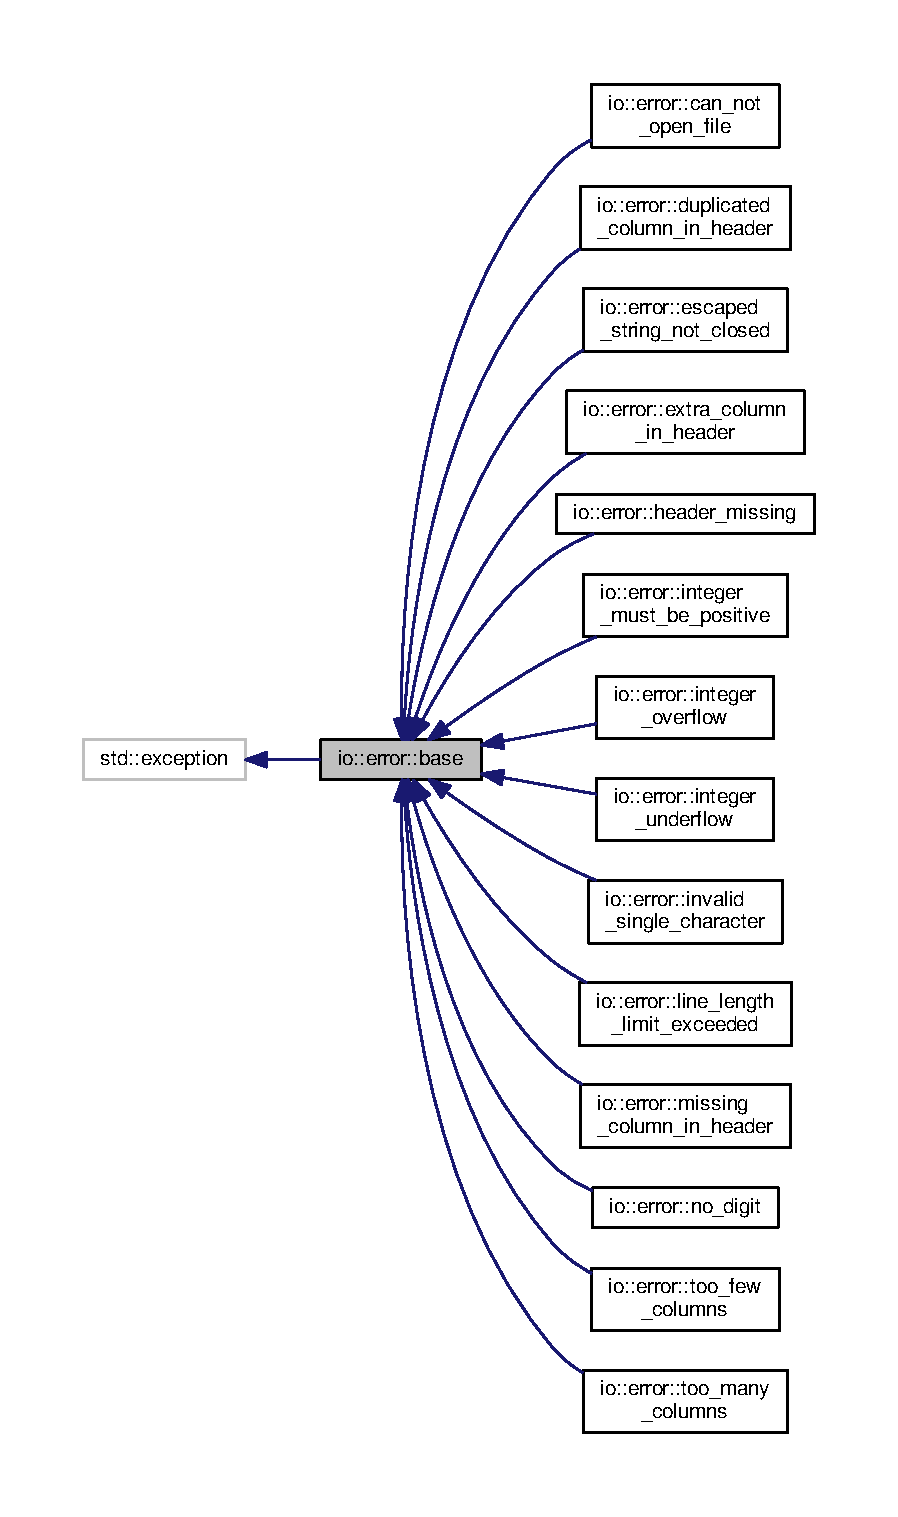
\includegraphics[height=550pt]{structio_1_1error_1_1base__inherit__graph}
\end{center}
\end{figure}


Collaboration diagram for io\+:\+:error\+:\+:base\+:\nopagebreak
\begin{figure}[H]
\begin{center}
\leavevmode
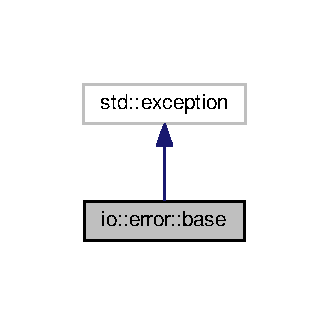
\includegraphics[width=158pt]{structio_1_1error_1_1base__coll__graph}
\end{center}
\end{figure}
\subsection*{Public Member Functions}
\begin{DoxyCompactItemize}
\item 
virtual void {\bfseries format\+\_\+error\+\_\+message} () const =0\label{structio_1_1error_1_1base_a7d9ff6a31b716a24f056cf8a3e15191d}

\item 
const char $\ast$ {\bfseries what} () const   throw ()\label{structio_1_1error_1_1base_ad99d4a2459e51ce2c24707569c4a0df6}

\end{DoxyCompactItemize}
\subsection*{Public Attributes}
\begin{DoxyCompactItemize}
\item 
char {\bfseries error\+\_\+message\+\_\+buffer} [512]\label{structio_1_1error_1_1base_a3be516c4636b7b61133968cb8081c885}

\end{DoxyCompactItemize}


The documentation for this struct was generated from the following file\+:\begin{DoxyCompactItemize}
\item 
csv.\+h\end{DoxyCompactItemize}

\section{io\+:\+:Byte\+Source\+Base Class Reference}
\label{classio_1_1_byte_source_base}\index{io\+::\+Byte\+Source\+Base@{io\+::\+Byte\+Source\+Base}}


Inheritance diagram for io\+:\+:Byte\+Source\+Base\+:\nopagebreak
\begin{figure}[H]
\begin{center}
\leavevmode
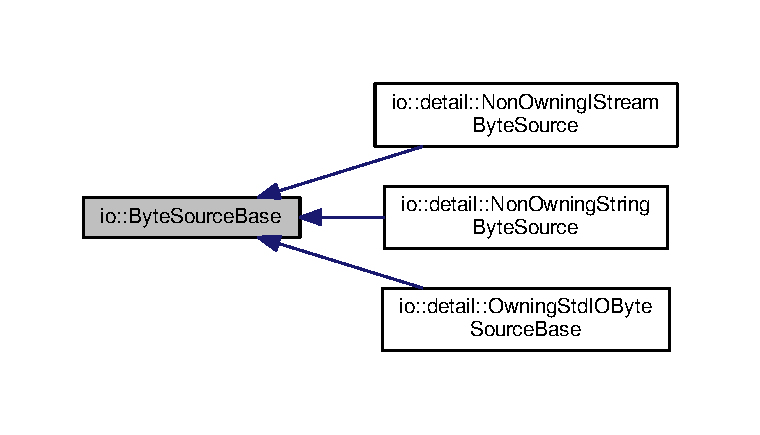
\includegraphics[width=350pt]{classio_1_1_byte_source_base__inherit__graph}
\end{center}
\end{figure}
\subsection*{Public Member Functions}
\begin{DoxyCompactItemize}
\item 
virtual int {\bfseries read} (char $\ast$buffer, int size)=0\label{classio_1_1_byte_source_base_a9598bcc869b79e44da07f0e6fa478615}

\end{DoxyCompactItemize}


The documentation for this class was generated from the following file\+:\begin{DoxyCompactItemize}
\item 
csv.\+h\end{DoxyCompactItemize}

\section{io\+:\+:error\+:\+:can\+\_\+not\+\_\+open\+\_\+file Struct Reference}
\label{structio_1_1error_1_1can__not__open__file}\index{io\+::error\+::can\+\_\+not\+\_\+open\+\_\+file@{io\+::error\+::can\+\_\+not\+\_\+open\+\_\+file}}


Inheritance diagram for io\+:\+:error\+:\+:can\+\_\+not\+\_\+open\+\_\+file\+:\nopagebreak
\begin{figure}[H]
\begin{center}
\leavevmode
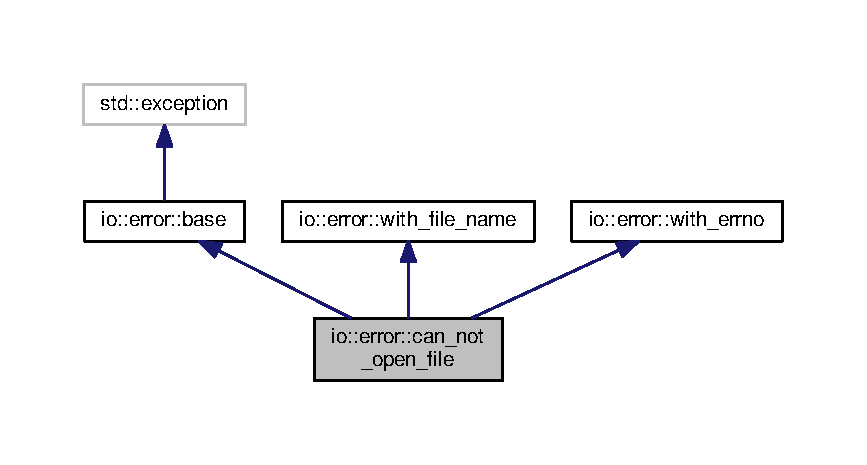
\includegraphics[width=350pt]{structio_1_1error_1_1can__not__open__file__inherit__graph}
\end{center}
\end{figure}


Collaboration diagram for io\+:\+:error\+:\+:can\+\_\+not\+\_\+open\+\_\+file\+:\nopagebreak
\begin{figure}[H]
\begin{center}
\leavevmode
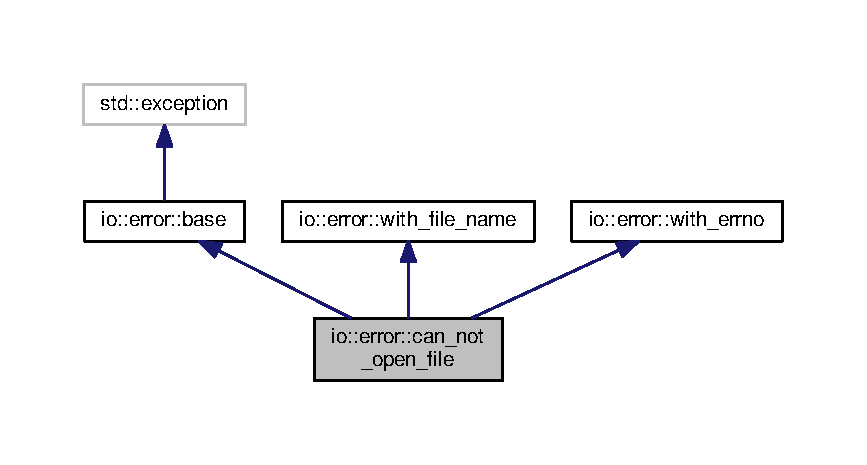
\includegraphics[width=350pt]{structio_1_1error_1_1can__not__open__file__coll__graph}
\end{center}
\end{figure}
\subsection*{Public Member Functions}
\begin{DoxyCompactItemize}
\item 
void {\bfseries format\+\_\+error\+\_\+message} () const \label{structio_1_1error_1_1can__not__open__file_a6b4f1a5ebfdbf12c6ee53c781c94b203}

\end{DoxyCompactItemize}
\subsection*{Additional Inherited Members}


The documentation for this struct was generated from the following file\+:\begin{DoxyCompactItemize}
\item 
csv.\+h\end{DoxyCompactItemize}

\section{io\+:\+:C\+S\+V\+Reader$<$ column\+\_\+count, trim\+\_\+policy, quote\+\_\+policy, overflow\+\_\+policy, comment\+\_\+policy $>$ Class Template Reference}
\label{classio_1_1_c_s_v_reader}\index{io\+::\+C\+S\+V\+Reader$<$ column\+\_\+count, trim\+\_\+policy, quote\+\_\+policy, overflow\+\_\+policy, comment\+\_\+policy $>$@{io\+::\+C\+S\+V\+Reader$<$ column\+\_\+count, trim\+\_\+policy, quote\+\_\+policy, overflow\+\_\+policy, comment\+\_\+policy $>$}}
\subsection*{Public Member Functions}
\begin{DoxyCompactItemize}
\item 
{\bfseries C\+S\+V\+Reader} (const {\bf C\+S\+V\+Reader} \&)=delete\label{classio_1_1_c_s_v_reader_a0507ac5abe201969a15df76795e13c28}

\item 
{\bf C\+S\+V\+Reader} \& {\bfseries operator=} (const {\bf C\+S\+V\+Reader} \&)\label{classio_1_1_c_s_v_reader_a37046e6629cf4254037c14440f14141d}

\item 
{\footnotesize template$<$class... Args$>$ }\\{\bfseries C\+S\+V\+Reader} (Args \&\&...args)\label{classio_1_1_c_s_v_reader_a189debf95672e7cd7582e9f73d7203e5}

\item 
char $\ast$ {\bfseries next\+\_\+line} ()\label{classio_1_1_c_s_v_reader_a9fec7797cb27f64360cc48adc5f32c72}

\item 
{\footnotesize template$<$class... Col\+Names$>$ }\\void {\bfseries read\+\_\+header} (ignore\+\_\+column ignore\+\_\+policy, Col\+Names...\+cols)\label{classio_1_1_c_s_v_reader_a9fad9ae02aa243dba6bc78156c5ce7e5}

\item 
{\footnotesize template$<$class... Col\+Names$>$ }\\void {\bfseries set\+\_\+header} (Col\+Names...\+cols)\label{classio_1_1_c_s_v_reader_ab68eedff1bd59a49fa4ddb160dff94e0}

\item 
bool {\bfseries has\+\_\+column} (const std\+::string \&name) const \label{classio_1_1_c_s_v_reader_a67c1d0d621fc0e4b8021d805dae9c176}

\item 
void {\bfseries set\+\_\+file\+\_\+name} (const std\+::string \&file\+\_\+name)\label{classio_1_1_c_s_v_reader_a4096c1e43a4fba2b4f5ae21d047b5fbc}

\item 
void {\bfseries set\+\_\+file\+\_\+name} (const char $\ast$file\+\_\+name)\label{classio_1_1_c_s_v_reader_a5f1dc083a8fa8661f5ecdcf6aebc7b24}

\item 
const char $\ast$ {\bfseries get\+\_\+truncated\+\_\+file\+\_\+name} () const \label{classio_1_1_c_s_v_reader_a7802939e9c108c4acfc7101baf52da95}

\item 
void {\bfseries set\+\_\+file\+\_\+line} (unsigned file\+\_\+line)\label{classio_1_1_c_s_v_reader_a1303bd6a2eb0d3d7c743212e52839ac4}

\item 
unsigned {\bfseries get\+\_\+file\+\_\+line} () const \label{classio_1_1_c_s_v_reader_aeea0f1ab9791a7dd3c699398c85edfaa}

\item 
{\footnotesize template$<$class... Col\+Type$>$ }\\bool {\bfseries read\+\_\+row} (Col\+Type \&...cols)\label{classio_1_1_c_s_v_reader_a61ecdcaa62c024bf97c4e5d133478d7e}

\end{DoxyCompactItemize}


The documentation for this class was generated from the following file\+:\begin{DoxyCompactItemize}
\item 
csv.\+h\end{DoxyCompactItemize}

\section{io\+:\+:double\+\_\+quote\+\_\+escape$<$ sep, quote $>$ Struct Template Reference}
\label{structio_1_1double__quote__escape}\index{io\+::double\+\_\+quote\+\_\+escape$<$ sep, quote $>$@{io\+::double\+\_\+quote\+\_\+escape$<$ sep, quote $>$}}
\subsection*{Static Public Member Functions}
\begin{DoxyCompactItemize}
\item 
static const char $\ast$ {\bfseries find\+\_\+next\+\_\+column\+\_\+end} (const char $\ast$col\+\_\+begin)\label{structio_1_1double__quote__escape_a30070914039ca8a20f716fbf53d68c41}

\item 
static void {\bfseries unescape} (char $\ast$\&col\+\_\+begin, char $\ast$\&col\+\_\+end)\label{structio_1_1double__quote__escape_a02e332751916fbdb7b35c238d690e580}

\end{DoxyCompactItemize}


The documentation for this struct was generated from the following file\+:\begin{DoxyCompactItemize}
\item 
csv.\+h\end{DoxyCompactItemize}

\section{io\+:\+:error\+:\+:duplicated\+\_\+column\+\_\+in\+\_\+header Struct Reference}
\label{structio_1_1error_1_1duplicated__column__in__header}\index{io\+::error\+::duplicated\+\_\+column\+\_\+in\+\_\+header@{io\+::error\+::duplicated\+\_\+column\+\_\+in\+\_\+header}}


Inheritance diagram for io\+:\+:error\+:\+:duplicated\+\_\+column\+\_\+in\+\_\+header\+:\nopagebreak
\begin{figure}[H]
\begin{center}
\leavevmode
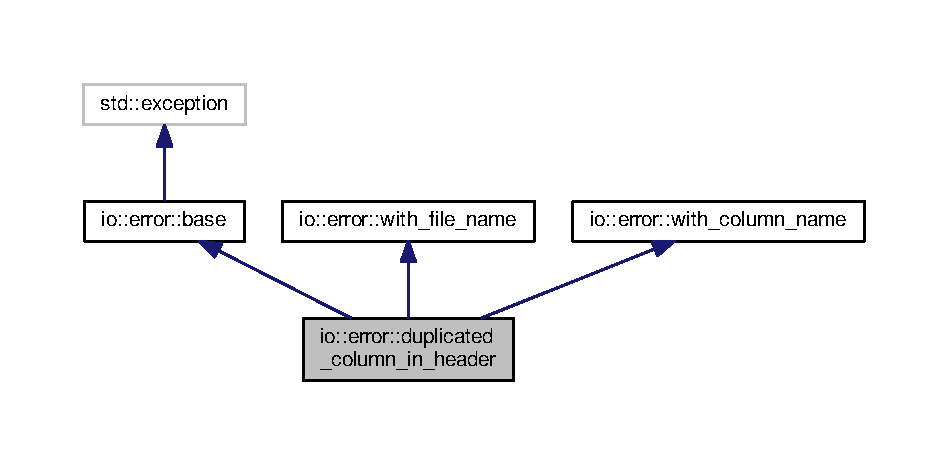
\includegraphics[width=350pt]{structio_1_1error_1_1duplicated__column__in__header__inherit__graph}
\end{center}
\end{figure}


Collaboration diagram for io\+:\+:error\+:\+:duplicated\+\_\+column\+\_\+in\+\_\+header\+:\nopagebreak
\begin{figure}[H]
\begin{center}
\leavevmode
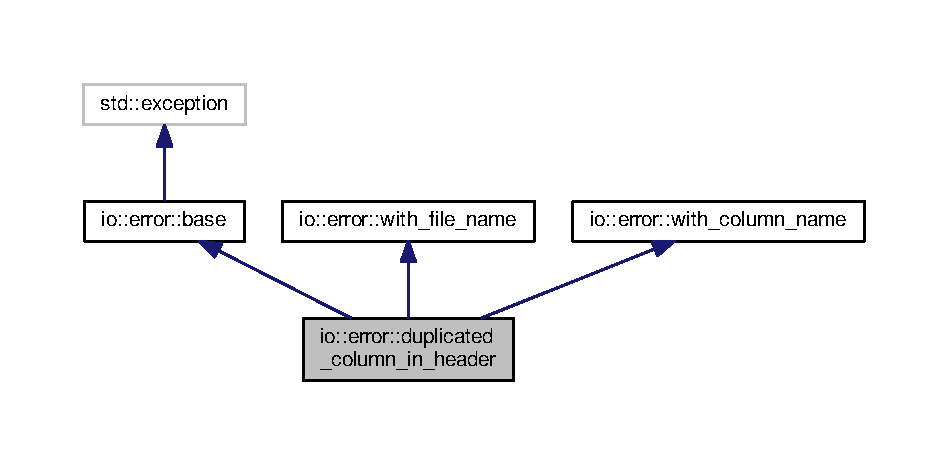
\includegraphics[width=350pt]{structio_1_1error_1_1duplicated__column__in__header__coll__graph}
\end{center}
\end{figure}
\subsection*{Public Member Functions}
\begin{DoxyCompactItemize}
\item 
void {\bfseries format\+\_\+error\+\_\+message} () const \label{structio_1_1error_1_1duplicated__column__in__header_aaaae2e6a92ea64017d76cf5972bd8e49}

\end{DoxyCompactItemize}
\subsection*{Additional Inherited Members}


The documentation for this struct was generated from the following file\+:\begin{DoxyCompactItemize}
\item 
csv.\+h\end{DoxyCompactItemize}

\section{io\+:\+:empty\+\_\+line\+\_\+comment Struct Reference}
\label{structio_1_1empty__line__comment}\index{io\+::empty\+\_\+line\+\_\+comment@{io\+::empty\+\_\+line\+\_\+comment}}
\subsection*{Static Public Member Functions}
\begin{DoxyCompactItemize}
\item 
static bool {\bfseries is\+\_\+comment} (const char $\ast$line)\label{structio_1_1empty__line__comment_a88e2cee044a9aafabf3e2a0e64fa5289}

\end{DoxyCompactItemize}


The documentation for this struct was generated from the following file\+:\begin{DoxyCompactItemize}
\item 
csv.\+h\end{DoxyCompactItemize}

\section{io\+:\+:error\+:\+:escaped\+\_\+string\+\_\+not\+\_\+closed Struct Reference}
\label{structio_1_1error_1_1escaped__string__not__closed}\index{io\+::error\+::escaped\+\_\+string\+\_\+not\+\_\+closed@{io\+::error\+::escaped\+\_\+string\+\_\+not\+\_\+closed}}


Inheritance diagram for io\+:\+:error\+:\+:escaped\+\_\+string\+\_\+not\+\_\+closed\+:\nopagebreak
\begin{figure}[H]
\begin{center}
\leavevmode
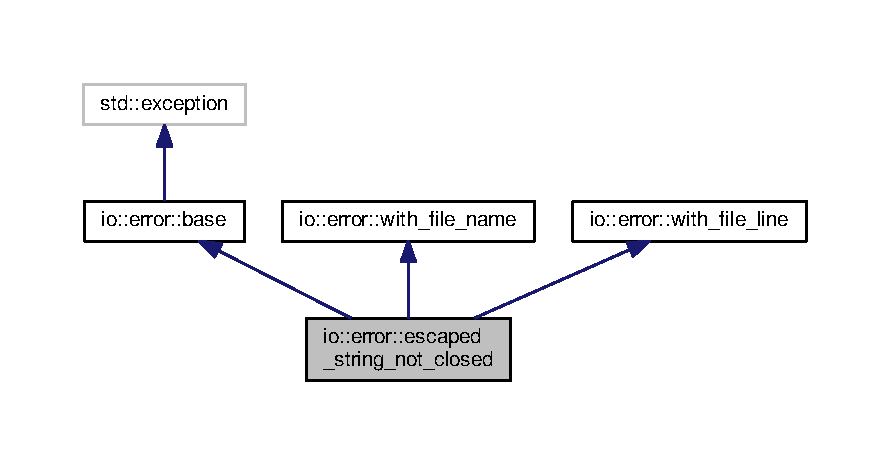
\includegraphics[width=350pt]{structio_1_1error_1_1escaped__string__not__closed__inherit__graph}
\end{center}
\end{figure}


Collaboration diagram for io\+:\+:error\+:\+:escaped\+\_\+string\+\_\+not\+\_\+closed\+:\nopagebreak
\begin{figure}[H]
\begin{center}
\leavevmode
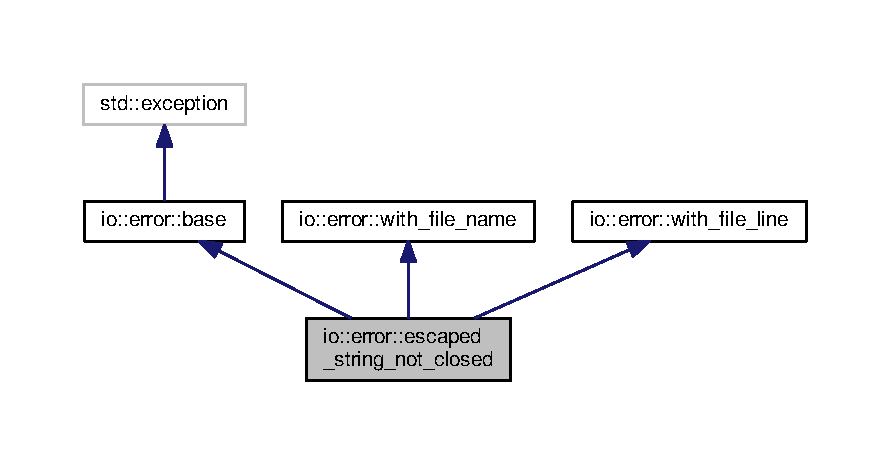
\includegraphics[width=350pt]{structio_1_1error_1_1escaped__string__not__closed__coll__graph}
\end{center}
\end{figure}
\subsection*{Public Member Functions}
\begin{DoxyCompactItemize}
\item 
void {\bfseries format\+\_\+error\+\_\+message} () const \label{structio_1_1error_1_1escaped__string__not__closed_a0dbbad1f20b62e2e43309c3f2ac0cc02}

\end{DoxyCompactItemize}
\subsection*{Additional Inherited Members}


The documentation for this struct was generated from the following file\+:\begin{DoxyCompactItemize}
\item 
csv.\+h\end{DoxyCompactItemize}

\section{io\+:\+:error\+:\+:extra\+\_\+column\+\_\+in\+\_\+header Struct Reference}
\label{structio_1_1error_1_1extra__column__in__header}\index{io\+::error\+::extra\+\_\+column\+\_\+in\+\_\+header@{io\+::error\+::extra\+\_\+column\+\_\+in\+\_\+header}}


Inheritance diagram for io\+:\+:error\+:\+:extra\+\_\+column\+\_\+in\+\_\+header\+:\nopagebreak
\begin{figure}[H]
\begin{center}
\leavevmode
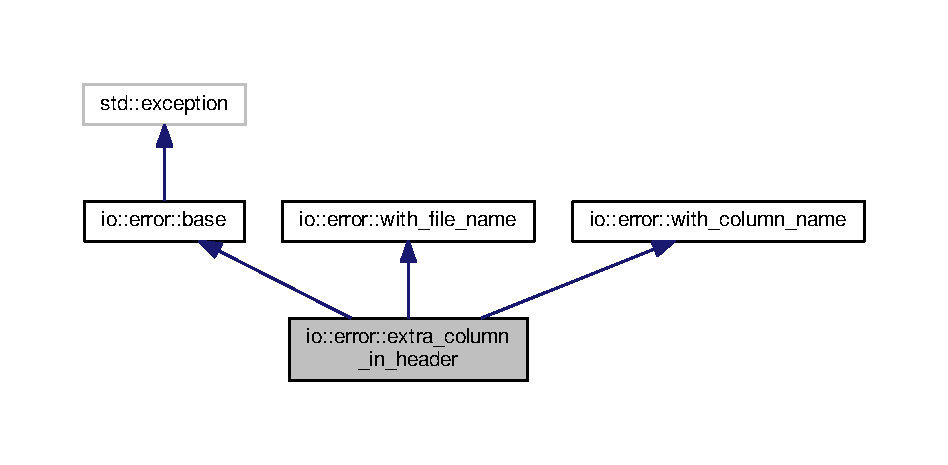
\includegraphics[width=350pt]{structio_1_1error_1_1extra__column__in__header__inherit__graph}
\end{center}
\end{figure}


Collaboration diagram for io\+:\+:error\+:\+:extra\+\_\+column\+\_\+in\+\_\+header\+:\nopagebreak
\begin{figure}[H]
\begin{center}
\leavevmode
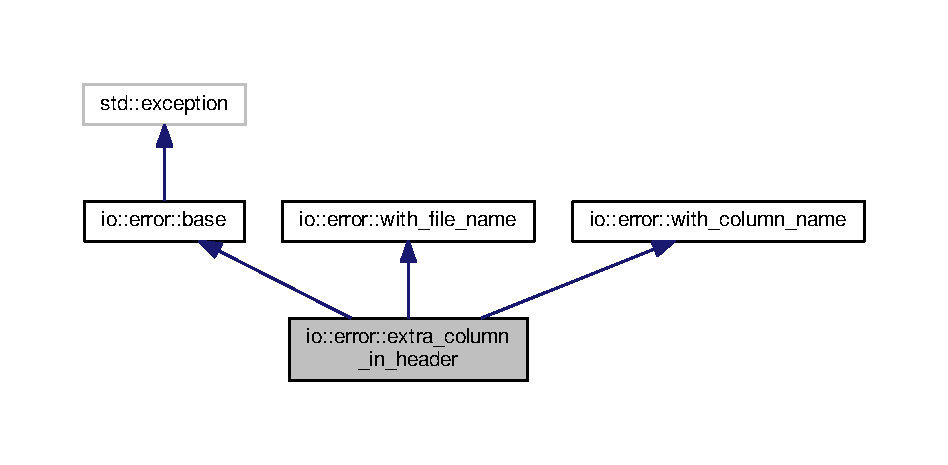
\includegraphics[width=350pt]{structio_1_1error_1_1extra__column__in__header__coll__graph}
\end{center}
\end{figure}
\subsection*{Public Member Functions}
\begin{DoxyCompactItemize}
\item 
void {\bfseries format\+\_\+error\+\_\+message} () const \label{structio_1_1error_1_1extra__column__in__header_a9cc12589f136ed7f9fc40802b9185d79}

\end{DoxyCompactItemize}
\subsection*{Additional Inherited Members}


The documentation for this struct was generated from the following file\+:\begin{DoxyCompactItemize}
\item 
csv.\+h\end{DoxyCompactItemize}

\section{Hash\+Table$<$ T $>$ Class Template Reference}
\label{class_hash_table}\index{Hash\+Table$<$ T $>$@{Hash\+Table$<$ T $>$}}
\subsection*{Public Member Functions}
\begin{DoxyCompactItemize}
\item 
{\bf Hash\+Table} ()\label{class_hash_table_aef9a69291686266a617009ace9bcb135}

\begin{DoxyCompactList}\small\item\em \doxyref{Hash\+Table$<$\+T$>$\+::\+Hash\+Table}{p.}{class_hash_table_aef9a69291686266a617009ace9bcb135} Fills values of array or vectors with empty objects. \end{DoxyCompactList}\item 
int {\bf total\+Entries} ()
\begin{DoxyCompactList}\small\item\em \doxyref{Hash\+Table$<$\+T$>$\+::total\+Entries}{p.}{class_hash_table_a1d554c7e56aa3f2c00bba4f01afd165c}. \end{DoxyCompactList}\item 
void {\bf add} (T \&, std\+::string)
\begin{DoxyCompactList}\small\item\em \doxyref{Hash\+Table$<$\+T$>$\+::add}{p.}{class_hash_table_a0f21a11fd44f462acb8905c56881325a}. \end{DoxyCompactList}\item 
T $\ast$ {\bf find} (std\+::string)
\begin{DoxyCompactList}\small\item\em \doxyref{Hash\+Table$<$\+T$>$\+::find}{p.}{class_hash_table_af1f049c6f33338d92be20746c4f10e22}. \end{DoxyCompactList}\item 
void {\bf clear} ()\label{class_hash_table_a50d0ee002ac774ac4b9a5c3c42e78564}

\begin{DoxyCompactList}\small\item\em \doxyref{Hash\+Table$<$\+T$>$\+::clear}{p.}{class_hash_table_a50d0ee002ac774ac4b9a5c3c42e78564} clears all values in the hash table. \end{DoxyCompactList}\end{DoxyCompactItemize}


\subsection{Member Function Documentation}
\index{Hash\+Table@{Hash\+Table}!add@{add}}
\index{add@{add}!Hash\+Table@{Hash\+Table}}
\subsubsection[{add(\+T \&, std\+::string)}]{\setlength{\rightskip}{0pt plus 5cm}template$<$class T$>$ void {\bf Hash\+Table}$<$ T $>$\+::add (
\begin{DoxyParamCaption}
\item[{T \&}]{e, }
\item[{std\+::string}]{tag}
\end{DoxyParamCaption}
)}\label{class_hash_table_a0f21a11fd44f462acb8905c56881325a}


\doxyref{Hash\+Table$<$\+T$>$\+::add}{p.}{class_hash_table_a0f21a11fd44f462acb8905c56881325a}. 


\begin{DoxyParams}{Parameters}
{\em e} & \\
\hline
{\em tag} & Adds value if the value is not found \\
\hline
\end{DoxyParams}
\index{Hash\+Table@{Hash\+Table}!find@{find}}
\index{find@{find}!Hash\+Table@{Hash\+Table}}
\subsubsection[{find(std\+::string)}]{\setlength{\rightskip}{0pt plus 5cm}template$<$class T $>$ T $\ast$ {\bf Hash\+Table}$<$ T $>$\+::find (
\begin{DoxyParamCaption}
\item[{std\+::string}]{s}
\end{DoxyParamCaption}
)}\label{class_hash_table_af1f049c6f33338d92be20746c4f10e22}


\doxyref{Hash\+Table$<$\+T$>$\+::find}{p.}{class_hash_table_af1f049c6f33338d92be20746c4f10e22}. 


\begin{DoxyParams}{Parameters}
{\em s} & \\
\hline
\end{DoxyParams}
\begin{DoxyReturn}{Returns}
Returns the templated object found at hash value if string is equal to value Returns nullptr if the value is not found 
\end{DoxyReturn}
\index{Hash\+Table@{Hash\+Table}!total\+Entries@{total\+Entries}}
\index{total\+Entries@{total\+Entries}!Hash\+Table@{Hash\+Table}}
\subsubsection[{total\+Entries()}]{\setlength{\rightskip}{0pt plus 5cm}template$<$class T $>$ int {\bf Hash\+Table}$<$ T $>$\+::total\+Entries (
\begin{DoxyParamCaption}
{}
\end{DoxyParamCaption}
)}\label{class_hash_table_a1d554c7e56aa3f2c00bba4f01afd165c}


\doxyref{Hash\+Table$<$\+T$>$\+::total\+Entries}{p.}{class_hash_table_a1d554c7e56aa3f2c00bba4f01afd165c}. 

\begin{DoxyReturn}{Returns}
returns the total entries into the hash table 
\end{DoxyReturn}


The documentation for this class was generated from the following file\+:\begin{DoxyCompactItemize}
\item 
Hash\+Table.\+h\end{DoxyCompactItemize}

\section{io\+:\+:error\+:\+:header\+\_\+missing Struct Reference}
\label{structio_1_1error_1_1header__missing}\index{io\+::error\+::header\+\_\+missing@{io\+::error\+::header\+\_\+missing}}


Inheritance diagram for io\+:\+:error\+:\+:header\+\_\+missing\+:\nopagebreak
\begin{figure}[H]
\begin{center}
\leavevmode
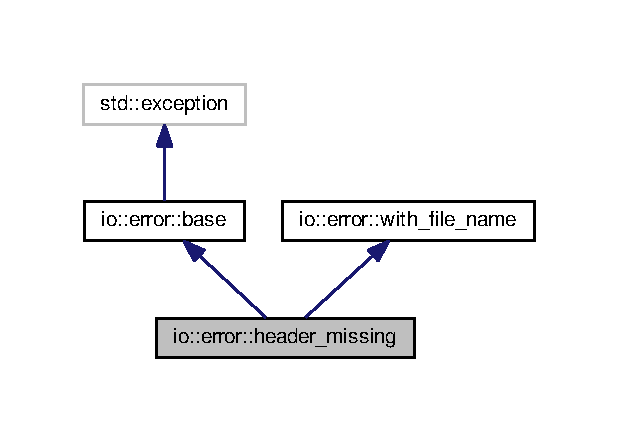
\includegraphics[width=297pt]{structio_1_1error_1_1header__missing__inherit__graph}
\end{center}
\end{figure}


Collaboration diagram for io\+:\+:error\+:\+:header\+\_\+missing\+:\nopagebreak
\begin{figure}[H]
\begin{center}
\leavevmode
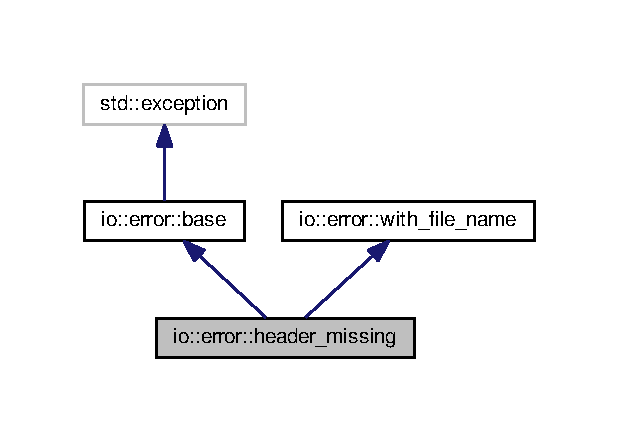
\includegraphics[width=297pt]{structio_1_1error_1_1header__missing__coll__graph}
\end{center}
\end{figure}
\subsection*{Public Member Functions}
\begin{DoxyCompactItemize}
\item 
void {\bfseries format\+\_\+error\+\_\+message} () const \label{structio_1_1error_1_1header__missing_a6e41864c2634db36dd0204251bffe512}

\end{DoxyCompactItemize}
\subsection*{Additional Inherited Members}


The documentation for this struct was generated from the following file\+:\begin{DoxyCompactItemize}
\item 
csv.\+h\end{DoxyCompactItemize}

\section{io\+:\+:ignore\+\_\+overflow Struct Reference}
\label{structio_1_1ignore__overflow}\index{io\+::ignore\+\_\+overflow@{io\+::ignore\+\_\+overflow}}
\subsection*{Static Public Member Functions}
\begin{DoxyCompactItemize}
\item 
{\footnotesize template$<$class T $>$ }\\static void {\bfseries on\+\_\+overflow} (T \&)\label{structio_1_1ignore__overflow_aed3e5026cfa7157ea9270ae377d1026b}

\item 
{\footnotesize template$<$class T $>$ }\\static void {\bfseries on\+\_\+underflow} (T \&)\label{structio_1_1ignore__overflow_aece692f7a20933149ec99aa1f97458ad}

\end{DoxyCompactItemize}


The documentation for this struct was generated from the following file\+:\begin{DoxyCompactItemize}
\item 
csv.\+h\end{DoxyCompactItemize}

\section{Indexer Class Reference}
\label{class_indexer}\index{Indexer@{Indexer}}


Collaboration diagram for Indexer\+:\nopagebreak
\begin{figure}[H]
\begin{center}
\leavevmode
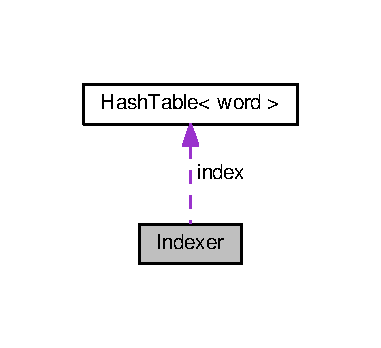
\includegraphics[width=183pt]{class_indexer__coll__graph}
\end{center}
\end{figure}
\subsection*{Public Member Functions}
\begin{DoxyCompactItemize}
\item 
void {\bf get\+Stop\+Words} ()\label{class_indexer_a8e0b420e8e47cef08c1b23869bb20add}

\begin{DoxyCompactList}\small\item\em \doxyref{Indexer\+::get\+Stop\+Words}{p.}{class_indexer_a8e0b420e8e47cef08c1b23869bb20add} Reads in the stop words. \end{DoxyCompactList}\item 
int {\bfseries get\+Total\+Words} ()\label{class_indexer_a41ec0dd75ccd821b51964ca4ec64eac8}

\item 
{\bf Indexer} ()\label{class_indexer_ac4c8c21c68d62185ceddbad8781e3b67}

\begin{DoxyCompactList}\small\item\em \doxyref{Indexer\+::\+Indexer}{p.}{class_indexer_ac4c8c21c68d62185ceddbad8781e3b67} Constructor for indexer. \end{DoxyCompactList}\item 
{\bf $\sim$\+Indexer} ()\label{class_indexer_aaf5971639a7a2e3d9af4d8da62deb6f4}

\begin{DoxyCompactList}\small\item\em \doxyref{Indexer\+::$\sim$\+Indexer}{p.}{class_indexer_aaf5971639a7a2e3d9af4d8da62deb6f4}. \end{DoxyCompactList}\item 
{\bf Indexer} ({\bf Hash\+Table}$<$ {\bf word} $>$ $\ast$i)
\begin{DoxyCompactList}\small\item\em \doxyref{Indexer\+::\+Indexer}{p.}{class_indexer_ac4c8c21c68d62185ceddbad8781e3b67}. \end{DoxyCompactList}\item 
void {\bf read\+New\+Tag} (int \&input\+ID, string \&input\+Word)
\begin{DoxyCompactList}\small\item\em \doxyref{Indexer\+::read\+New\+Tag}{p.}{class_indexer_a3bfdc5a3b79b239b020995e7741ae0e4}. \end{DoxyCompactList}\item 
{\bf word} {\bf search\+Index} (string)
\begin{DoxyCompactList}\small\item\em \doxyref{Indexer\+::search\+Index}{p.}{class_indexer_ac08c04ca8fd501ded3d682581aca82a9}. \end{DoxyCompactList}\item 
void {\bf read\+New\+Word} (int \&input\+ID, string \&input\+Word)
\begin{DoxyCompactList}\small\item\em \doxyref{Indexer\+::read\+New\+Word}{p.}{class_indexer_a7217bd3ebc936bd672d3b741202d787c}. \end{DoxyCompactList}\end{DoxyCompactItemize}
\subsection*{Public Attributes}
\begin{DoxyCompactItemize}
\item 
{\bf Hash\+Table}$<$ {\bf word} $>$ $\ast$ {\bfseries index}\label{class_indexer_a0937c617b53483d6f234a49a63783cda}

\end{DoxyCompactItemize}


\subsection{Constructor \& Destructor Documentation}
\index{Indexer@{Indexer}!Indexer@{Indexer}}
\index{Indexer@{Indexer}!Indexer@{Indexer}}
\subsubsection[{Indexer(\+Hash\+Table$<$ word $>$ $\ast$i)}]{\setlength{\rightskip}{0pt plus 5cm}Indexer\+::\+Indexer (
\begin{DoxyParamCaption}
\item[{{\bf Hash\+Table}$<$ {\bf word} $>$ $\ast$}]{i}
\end{DoxyParamCaption}
)}\label{class_indexer_a547f91155632bf2da7b5505e19e3e553}


\doxyref{Indexer\+::\+Indexer}{p.}{class_indexer_ac4c8c21c68d62185ceddbad8781e3b67}. 


\begin{DoxyParams}{Parameters}
{\em i} & Constructor for overloaded hashtable \\
\hline
\end{DoxyParams}


\subsection{Member Function Documentation}
\index{Indexer@{Indexer}!read\+New\+Tag@{read\+New\+Tag}}
\index{read\+New\+Tag@{read\+New\+Tag}!Indexer@{Indexer}}
\subsubsection[{read\+New\+Tag(int \&input\+I\+D, string \&input\+Word)}]{\setlength{\rightskip}{0pt plus 5cm}void Indexer\+::read\+New\+Tag (
\begin{DoxyParamCaption}
\item[{int \&}]{input\+ID, }
\item[{string \&}]{input\+Tag}
\end{DoxyParamCaption}
)}\label{class_indexer_a3bfdc5a3b79b239b020995e7741ae0e4}


\doxyref{Indexer\+::read\+New\+Tag}{p.}{class_indexer_a3bfdc5a3b79b239b020995e7741ae0e4}. 


\begin{DoxyParams}{Parameters}
{\em input\+ID} & \\
\hline
{\em input\+Tag} & Adds tag files to index hashtable \\
\hline
\end{DoxyParams}


Here is the caller graph for this function\+:\nopagebreak
\begin{figure}[H]
\begin{center}
\leavevmode
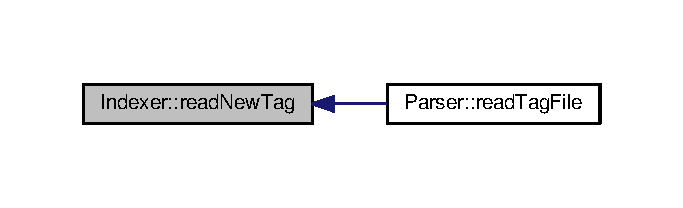
\includegraphics[width=328pt]{class_indexer_a3bfdc5a3b79b239b020995e7741ae0e4_icgraph}
\end{center}
\end{figure}


\index{Indexer@{Indexer}!read\+New\+Word@{read\+New\+Word}}
\index{read\+New\+Word@{read\+New\+Word}!Indexer@{Indexer}}
\subsubsection[{read\+New\+Word(int \&input\+I\+D, string \&input\+Word)}]{\setlength{\rightskip}{0pt plus 5cm}void Indexer\+::read\+New\+Word (
\begin{DoxyParamCaption}
\item[{int \&}]{input\+ID, }
\item[{string \&}]{input\+Word}
\end{DoxyParamCaption}
)}\label{class_indexer_a7217bd3ebc936bd672d3b741202d787c}


\doxyref{Indexer\+::read\+New\+Word}{p.}{class_indexer_a7217bd3ebc936bd672d3b741202d787c}. 


\begin{DoxyParams}{Parameters}
{\em input\+ID} & \\
\hline
{\em input\+Word} & Removes stop words Stems the word Adds the word to index Hashtable \\
\hline
\end{DoxyParams}


Here is the caller graph for this function\+:\nopagebreak
\begin{figure}[H]
\begin{center}
\leavevmode
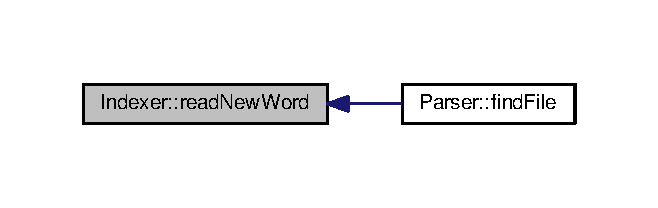
\includegraphics[width=316pt]{class_indexer_a7217bd3ebc936bd672d3b741202d787c_icgraph}
\end{center}
\end{figure}


\index{Indexer@{Indexer}!search\+Index@{search\+Index}}
\index{search\+Index@{search\+Index}!Indexer@{Indexer}}
\subsubsection[{search\+Index(string)}]{\setlength{\rightskip}{0pt plus 5cm}{\bf word} Indexer\+::search\+Index (
\begin{DoxyParamCaption}
\item[{string}]{t}
\end{DoxyParamCaption}
)}\label{class_indexer_ac08c04ca8fd501ded3d682581aca82a9}


\doxyref{Indexer\+::search\+Index}{p.}{class_indexer_ac08c04ca8fd501ded3d682581aca82a9}. 


\begin{DoxyParams}{Parameters}
{\em t} & \\
\hline
\end{DoxyParams}
\begin{DoxyReturn}{Returns}
Returns the word object for the string searched from the hash table 
\end{DoxyReturn}


Here is the caller graph for this function\+:\nopagebreak
\begin{figure}[H]
\begin{center}
\leavevmode
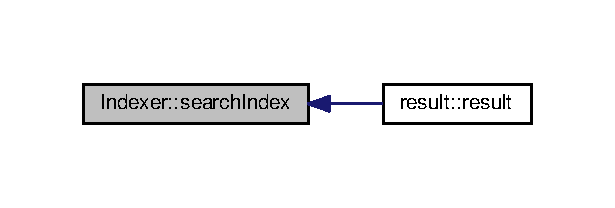
\includegraphics[width=295pt]{class_indexer_ac08c04ca8fd501ded3d682581aca82a9_icgraph}
\end{center}
\end{figure}




The documentation for this class was generated from the following files\+:\begin{DoxyCompactItemize}
\item 
Indexer.\+h\item 
Indexer.\+cpp\end{DoxyCompactItemize}

\section{Index\+Interface$<$ T $>$ Class Template Reference}
\label{class_index_interface}\index{Index\+Interface$<$ T $>$@{Index\+Interface$<$ T $>$}}
\subsection*{Public Member Functions}
\begin{DoxyCompactItemize}
\item 
virtual void {\bfseries add} (T, std\+::string)=0\label{class_index_interface_af565b2ad613b3506b1c51332f3d5c553}

\item 
virtual T $\ast$ {\bfseries find} (std\+::string)=0\label{class_index_interface_a2363614c8d270d26fef72c2b60293d14}

\end{DoxyCompactItemize}


The documentation for this class was generated from the following file\+:\begin{DoxyCompactItemize}
\item 
Index\+Interface.\+h\end{DoxyCompactItemize}

\section{io\+:\+:error\+:\+:integer\+\_\+must\+\_\+be\+\_\+positive Struct Reference}
\label{structio_1_1error_1_1integer__must__be__positive}\index{io\+::error\+::integer\+\_\+must\+\_\+be\+\_\+positive@{io\+::error\+::integer\+\_\+must\+\_\+be\+\_\+positive}}


Inheritance diagram for io\+:\+:error\+:\+:integer\+\_\+must\+\_\+be\+\_\+positive\+:\nopagebreak
\begin{figure}[H]
\begin{center}
\leavevmode
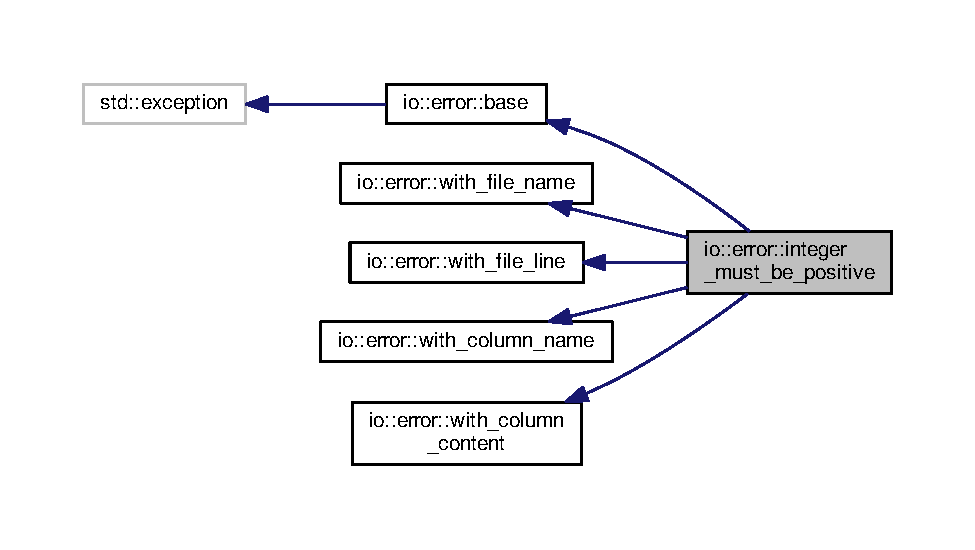
\includegraphics[width=350pt]{structio_1_1error_1_1integer__must__be__positive__inherit__graph}
\end{center}
\end{figure}


Collaboration diagram for io\+:\+:error\+:\+:integer\+\_\+must\+\_\+be\+\_\+positive\+:\nopagebreak
\begin{figure}[H]
\begin{center}
\leavevmode
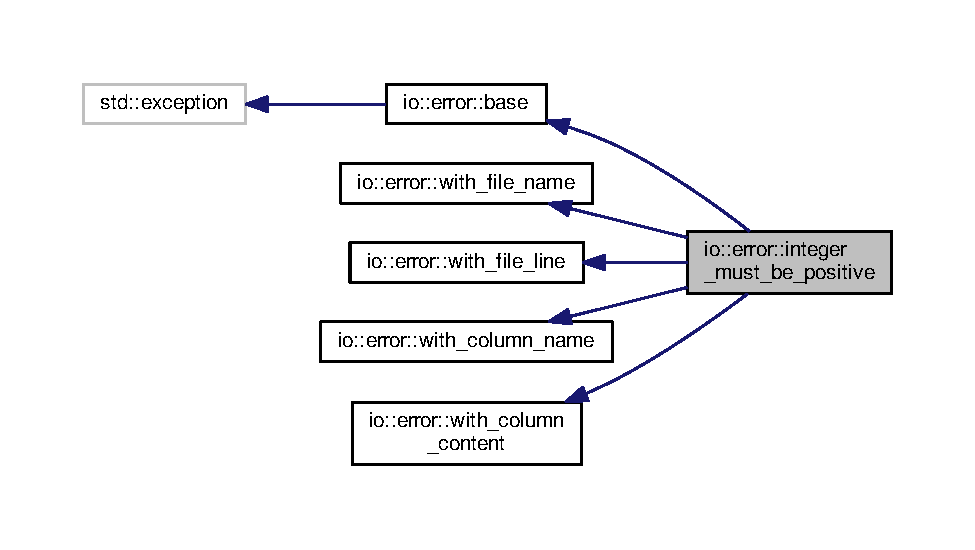
\includegraphics[width=350pt]{structio_1_1error_1_1integer__must__be__positive__coll__graph}
\end{center}
\end{figure}
\subsection*{Public Member Functions}
\begin{DoxyCompactItemize}
\item 
void {\bfseries format\+\_\+error\+\_\+message} () const \label{structio_1_1error_1_1integer__must__be__positive_a7150923d999e4d6cb9b6c4b5f1f51dfa}

\end{DoxyCompactItemize}
\subsection*{Additional Inherited Members}


The documentation for this struct was generated from the following file\+:\begin{DoxyCompactItemize}
\item 
csv.\+h\end{DoxyCompactItemize}

\section{io\+:\+:error\+:\+:integer\+\_\+overflow Struct Reference}
\label{structio_1_1error_1_1integer__overflow}\index{io\+::error\+::integer\+\_\+overflow@{io\+::error\+::integer\+\_\+overflow}}


Inheritance diagram for io\+:\+:error\+:\+:integer\+\_\+overflow\+:\nopagebreak
\begin{figure}[H]
\begin{center}
\leavevmode
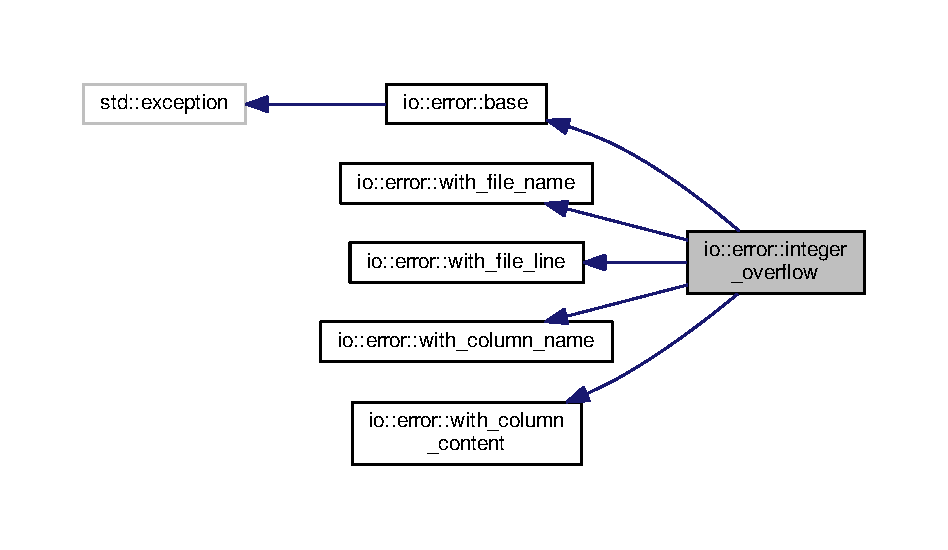
\includegraphics[width=350pt]{structio_1_1error_1_1integer__overflow__inherit__graph}
\end{center}
\end{figure}


Collaboration diagram for io\+:\+:error\+:\+:integer\+\_\+overflow\+:\nopagebreak
\begin{figure}[H]
\begin{center}
\leavevmode
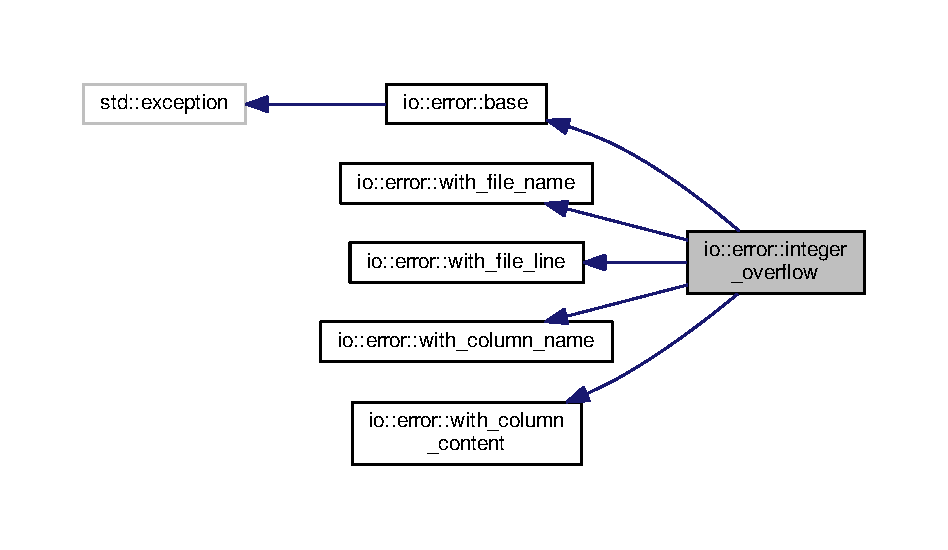
\includegraphics[width=350pt]{structio_1_1error_1_1integer__overflow__coll__graph}
\end{center}
\end{figure}
\subsection*{Public Member Functions}
\begin{DoxyCompactItemize}
\item 
void {\bfseries format\+\_\+error\+\_\+message} () const \label{structio_1_1error_1_1integer__overflow_a5fa7e6154c54a7d020f329c1816ab746}

\end{DoxyCompactItemize}
\subsection*{Additional Inherited Members}


The documentation for this struct was generated from the following file\+:\begin{DoxyCompactItemize}
\item 
csv.\+h\end{DoxyCompactItemize}

\section{io\+:\+:error\+:\+:integer\+\_\+underflow Struct Reference}
\label{structio_1_1error_1_1integer__underflow}\index{io\+::error\+::integer\+\_\+underflow@{io\+::error\+::integer\+\_\+underflow}}


Inheritance diagram for io\+:\+:error\+:\+:integer\+\_\+underflow\+:\nopagebreak
\begin{figure}[H]
\begin{center}
\leavevmode
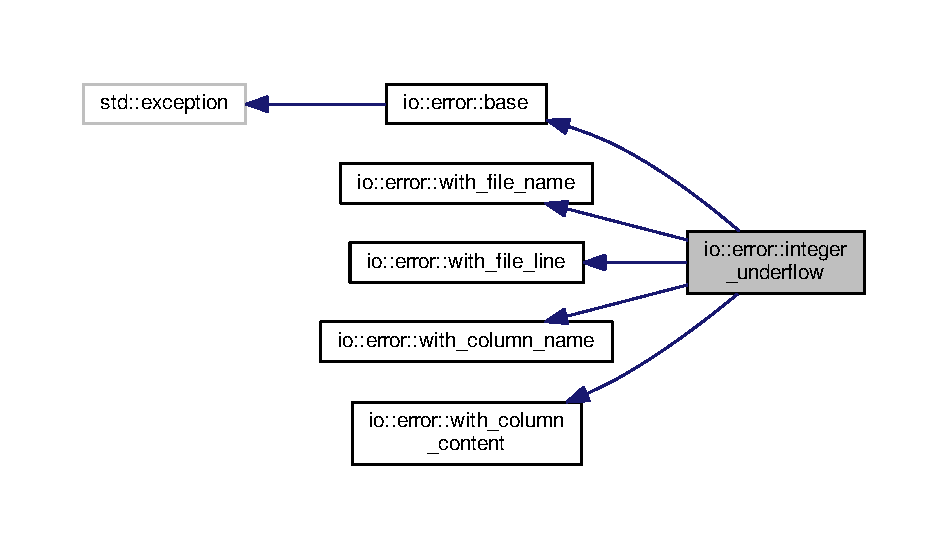
\includegraphics[width=350pt]{structio_1_1error_1_1integer__underflow__inherit__graph}
\end{center}
\end{figure}


Collaboration diagram for io\+:\+:error\+:\+:integer\+\_\+underflow\+:\nopagebreak
\begin{figure}[H]
\begin{center}
\leavevmode
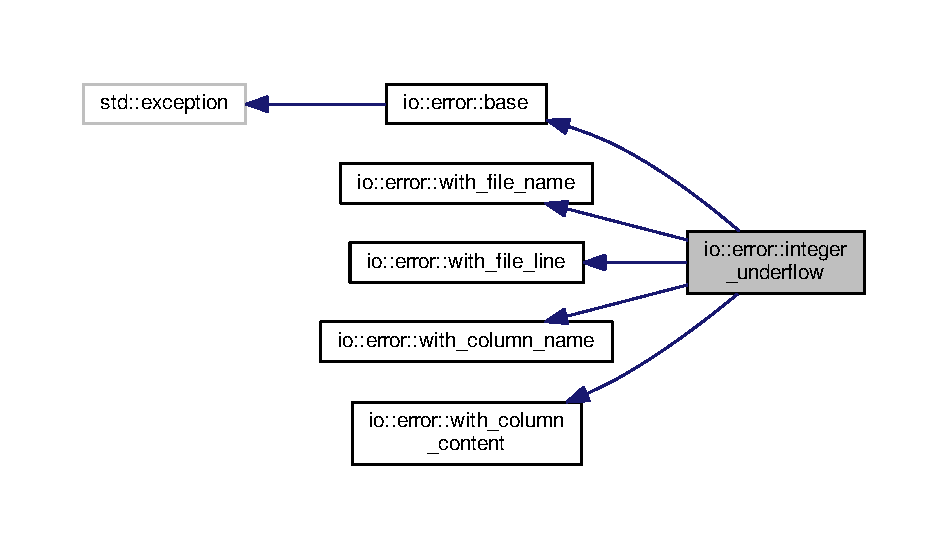
\includegraphics[width=350pt]{structio_1_1error_1_1integer__underflow__coll__graph}
\end{center}
\end{figure}
\subsection*{Public Member Functions}
\begin{DoxyCompactItemize}
\item 
void {\bfseries format\+\_\+error\+\_\+message} () const \label{structio_1_1error_1_1integer__underflow_adb68f28b47254f5dd855a2437bcaabae}

\end{DoxyCompactItemize}
\subsection*{Additional Inherited Members}


The documentation for this struct was generated from the following file\+:\begin{DoxyCompactItemize}
\item 
csv.\+h\end{DoxyCompactItemize}

\section{io\+:\+:error\+:\+:invalid\+\_\+single\+\_\+character Struct Reference}
\label{structio_1_1error_1_1invalid__single__character}\index{io\+::error\+::invalid\+\_\+single\+\_\+character@{io\+::error\+::invalid\+\_\+single\+\_\+character}}


Inheritance diagram for io\+:\+:error\+:\+:invalid\+\_\+single\+\_\+character\+:\nopagebreak
\begin{figure}[H]
\begin{center}
\leavevmode
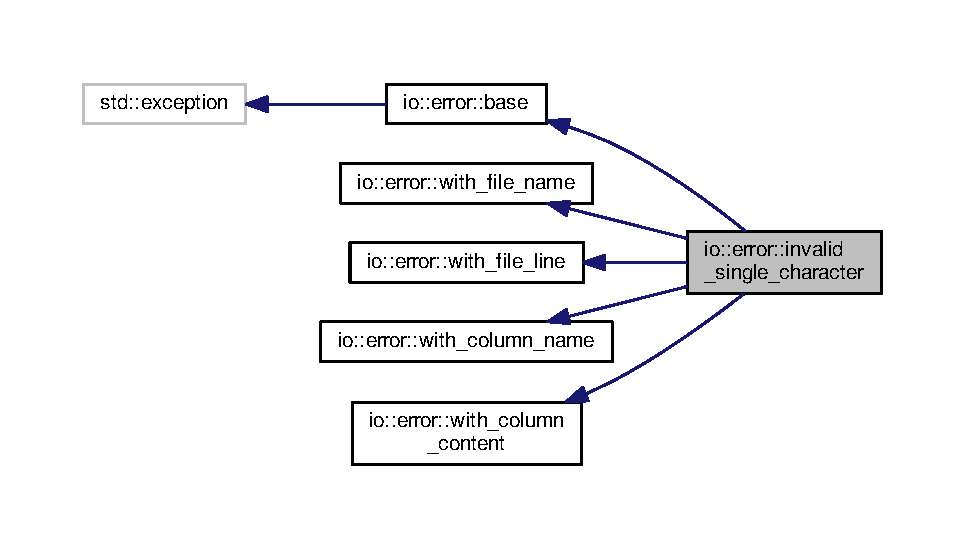
\includegraphics[width=350pt]{structio_1_1error_1_1invalid__single__character__inherit__graph}
\end{center}
\end{figure}


Collaboration diagram for io\+:\+:error\+:\+:invalid\+\_\+single\+\_\+character\+:\nopagebreak
\begin{figure}[H]
\begin{center}
\leavevmode
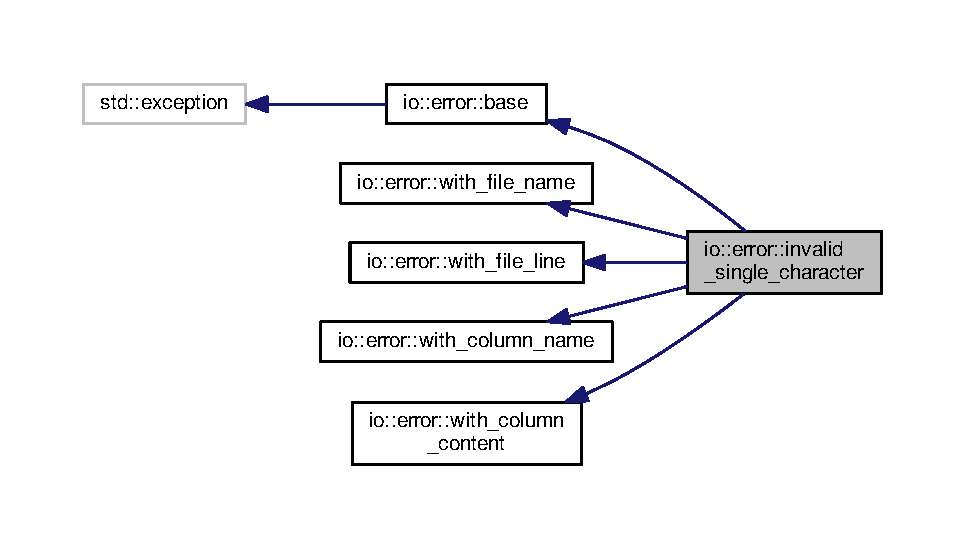
\includegraphics[width=350pt]{structio_1_1error_1_1invalid__single__character__coll__graph}
\end{center}
\end{figure}
\subsection*{Public Member Functions}
\begin{DoxyCompactItemize}
\item 
void {\bfseries format\+\_\+error\+\_\+message} () const \label{structio_1_1error_1_1invalid__single__character_a071fa29c62051488d0fc7f51137ae3dc}

\end{DoxyCompactItemize}
\subsection*{Additional Inherited Members}


The documentation for this struct was generated from the following file\+:\begin{DoxyCompactItemize}
\item 
csv.\+h\end{DoxyCompactItemize}

\section{io\+:\+:error\+:\+:line\+\_\+length\+\_\+limit\+\_\+exceeded Struct Reference}
\label{structio_1_1error_1_1line__length__limit__exceeded}\index{io\+::error\+::line\+\_\+length\+\_\+limit\+\_\+exceeded@{io\+::error\+::line\+\_\+length\+\_\+limit\+\_\+exceeded}}


Inheritance diagram for io\+:\+:error\+:\+:line\+\_\+length\+\_\+limit\+\_\+exceeded\+:\nopagebreak
\begin{figure}[H]
\begin{center}
\leavevmode
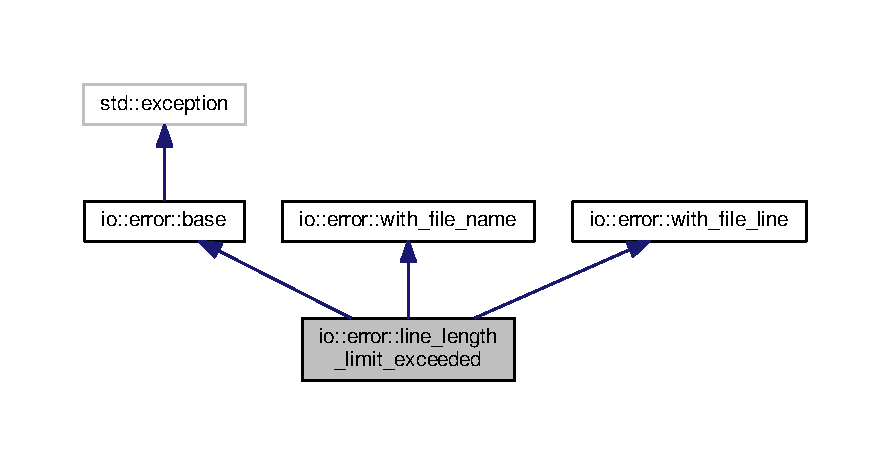
\includegraphics[width=350pt]{structio_1_1error_1_1line__length__limit__exceeded__inherit__graph}
\end{center}
\end{figure}


Collaboration diagram for io\+:\+:error\+:\+:line\+\_\+length\+\_\+limit\+\_\+exceeded\+:\nopagebreak
\begin{figure}[H]
\begin{center}
\leavevmode
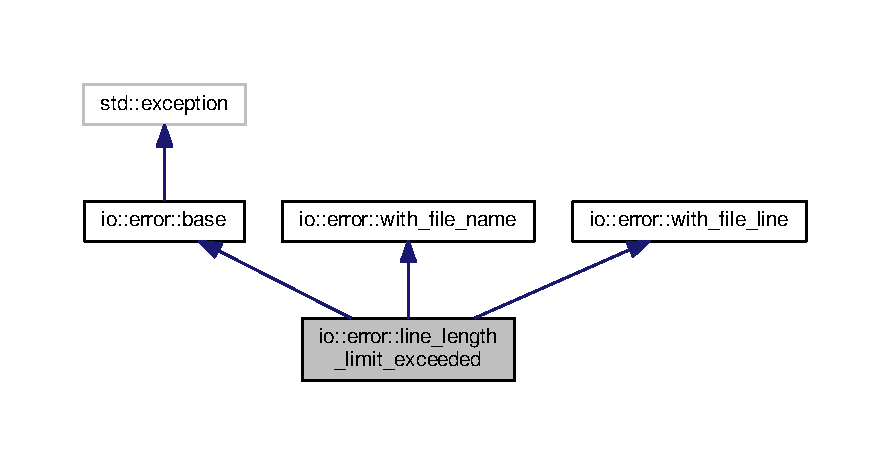
\includegraphics[width=350pt]{structio_1_1error_1_1line__length__limit__exceeded__coll__graph}
\end{center}
\end{figure}
\subsection*{Public Member Functions}
\begin{DoxyCompactItemize}
\item 
void {\bfseries format\+\_\+error\+\_\+message} () const \label{structio_1_1error_1_1line__length__limit__exceeded_aa7c12639e9f39f04ff1c8a53e8e41a06}

\end{DoxyCompactItemize}
\subsection*{Additional Inherited Members}


The documentation for this struct was generated from the following file\+:\begin{DoxyCompactItemize}
\item 
csv.\+h\end{DoxyCompactItemize}

\section{io\+:\+:Line\+Reader Class Reference}
\label{classio_1_1_line_reader}\index{io\+::\+Line\+Reader@{io\+::\+Line\+Reader}}
\subsection*{Public Member Functions}
\begin{DoxyCompactItemize}
\item 
{\bfseries Line\+Reader} (const {\bf Line\+Reader} \&)=delete\label{classio_1_1_line_reader_a84f2957de769bb701eaaddfd8bc004dd}

\item 
{\bf Line\+Reader} \& {\bfseries operator=} (const {\bf Line\+Reader} \&)=delete\label{classio_1_1_line_reader_a9ebd7beca16060ffc0ea8df3c0c6ff25}

\item 
{\bfseries Line\+Reader} (const char $\ast$file\+\_\+name)\label{classio_1_1_line_reader_a81a75d3f53725d35822f490007520e29}

\item 
{\bfseries Line\+Reader} (const std\+::string \&file\+\_\+name)\label{classio_1_1_line_reader_ab0eb26f44fa6b18f9c39dfb2561ac882}

\item 
{\bfseries Line\+Reader} (const char $\ast$file\+\_\+name, std\+::unique\+\_\+ptr$<$ {\bf Byte\+Source\+Base} $>$byte\+\_\+source)\label{classio_1_1_line_reader_af4ebb130a7d6c78356573f6d0304266c}

\item 
{\bfseries Line\+Reader} (const std\+::string \&file\+\_\+name, std\+::unique\+\_\+ptr$<$ {\bf Byte\+Source\+Base} $>$byte\+\_\+source)\label{classio_1_1_line_reader_ab625b3a8001dca811b0e211c6cfc1b28}

\item 
{\bfseries Line\+Reader} (const char $\ast$file\+\_\+name, const char $\ast$data\+\_\+begin, const char $\ast$data\+\_\+end)\label{classio_1_1_line_reader_ad5a65d6f23474884061a77ea858c042b}

\item 
{\bfseries Line\+Reader} (const std\+::string \&file\+\_\+name, const char $\ast$data\+\_\+begin, const char $\ast$data\+\_\+end)\label{classio_1_1_line_reader_a0a52d864b46442a253443cac1367366e}

\item 
{\bfseries Line\+Reader} (const char $\ast$file\+\_\+name, F\+I\+LE $\ast$file)\label{classio_1_1_line_reader_ad2a8943ba0848ae5052e2f5ad30c010e}

\item 
{\bfseries Line\+Reader} (const std\+::string \&file\+\_\+name, F\+I\+LE $\ast$file)\label{classio_1_1_line_reader_a93fa2e3ae98b0e7a7391714d6395c552}

\item 
{\bfseries Line\+Reader} (const char $\ast$file\+\_\+name, std\+::istream \&in)\label{classio_1_1_line_reader_a301c08eb9ca5d3fdccf4e9a8e5ac82f8}

\item 
{\bfseries Line\+Reader} (const std\+::string \&file\+\_\+name, std\+::istream \&in)\label{classio_1_1_line_reader_a3eacf4d1539a24122c6897fce4e72f06}

\item 
void {\bfseries set\+\_\+file\+\_\+name} (const std\+::string \&file\+\_\+name)\label{classio_1_1_line_reader_a1a0763d491dec16cebc33134e965dfee}

\item 
void {\bfseries set\+\_\+file\+\_\+name} (const char $\ast$file\+\_\+name)\label{classio_1_1_line_reader_a81c56ac68497da5ec874333ce063fd83}

\item 
const char $\ast$ {\bfseries get\+\_\+truncated\+\_\+file\+\_\+name} () const \label{classio_1_1_line_reader_a4a0ea19065c0092e7fc68c4ccbd815b1}

\item 
void {\bfseries set\+\_\+file\+\_\+line} (unsigned file\+\_\+line)\label{classio_1_1_line_reader_a581b55d4ced6adb964de50fa8ac6eb08}

\item 
unsigned {\bfseries get\+\_\+file\+\_\+line} () const \label{classio_1_1_line_reader_ae043da5b943a08601246c7e3420fd126}

\item 
char $\ast$ {\bfseries next\+\_\+line} ()\label{classio_1_1_line_reader_a97f4e0129611d9da2b8c966ffe670be5}

\end{DoxyCompactItemize}


The documentation for this class was generated from the following file\+:\begin{DoxyCompactItemize}
\item 
csv.\+h\end{DoxyCompactItemize}

\section{Main\+Window Class Reference}
\label{class_main_window}\index{Main\+Window@{Main\+Window}}


Inheritance diagram for Main\+Window\+:\nopagebreak
\begin{figure}[H]
\begin{center}
\leavevmode
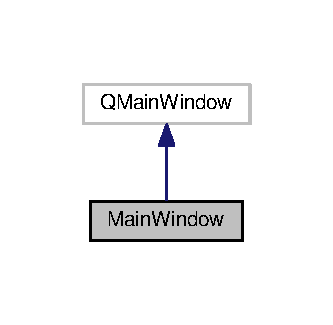
\includegraphics[width=160pt]{class_main_window__inherit__graph}
\end{center}
\end{figure}


Collaboration diagram for Main\+Window\+:\nopagebreak
\begin{figure}[H]
\begin{center}
\leavevmode
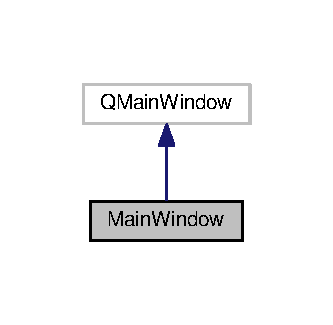
\includegraphics[width=160pt]{class_main_window__coll__graph}
\end{center}
\end{figure}
\subsection*{Public Member Functions}
\begin{DoxyCompactItemize}
\item 
{\bfseries Main\+Window} (Q\+Widget $\ast$parent=0)\label{class_main_window_a8b244be8b7b7db1b08de2a2acb9409db}

\end{DoxyCompactItemize}


The documentation for this class was generated from the following files\+:\begin{DoxyCompactItemize}
\item 
mainwindow.\+h\item 
mainwindow.\+cpp\end{DoxyCompactItemize}

\section{io\+:\+:error\+:\+:missing\+\_\+column\+\_\+in\+\_\+header Struct Reference}
\label{structio_1_1error_1_1missing__column__in__header}\index{io\+::error\+::missing\+\_\+column\+\_\+in\+\_\+header@{io\+::error\+::missing\+\_\+column\+\_\+in\+\_\+header}}


Inheritance diagram for io\+:\+:error\+:\+:missing\+\_\+column\+\_\+in\+\_\+header\+:\nopagebreak
\begin{figure}[H]
\begin{center}
\leavevmode
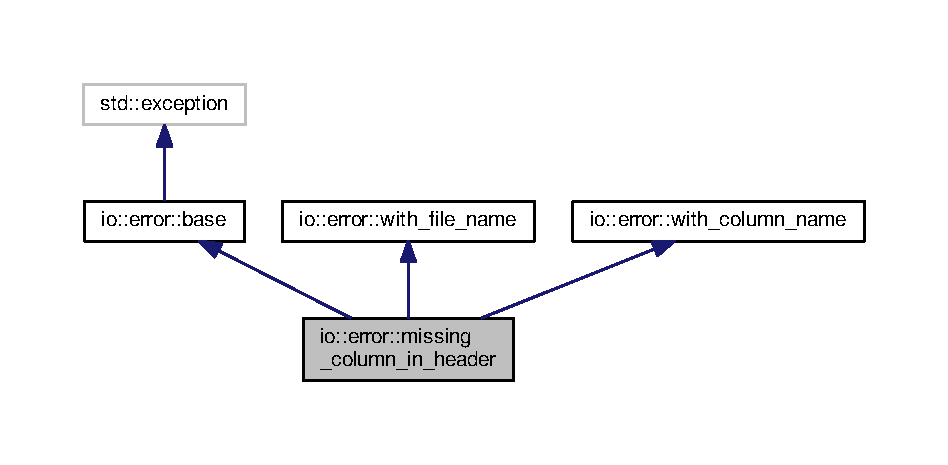
\includegraphics[width=350pt]{structio_1_1error_1_1missing__column__in__header__inherit__graph}
\end{center}
\end{figure}


Collaboration diagram for io\+:\+:error\+:\+:missing\+\_\+column\+\_\+in\+\_\+header\+:\nopagebreak
\begin{figure}[H]
\begin{center}
\leavevmode
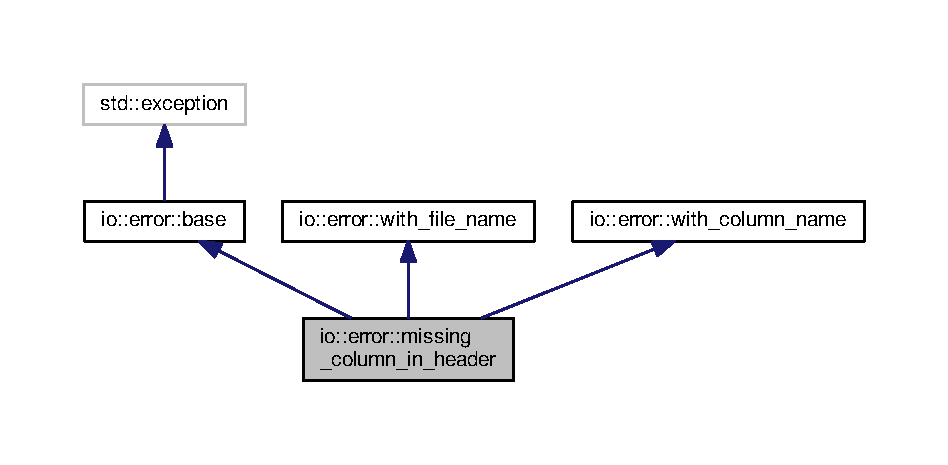
\includegraphics[width=350pt]{structio_1_1error_1_1missing__column__in__header__coll__graph}
\end{center}
\end{figure}
\subsection*{Public Member Functions}
\begin{DoxyCompactItemize}
\item 
void {\bfseries format\+\_\+error\+\_\+message} () const \label{structio_1_1error_1_1missing__column__in__header_acd0f4c75f6ffa54c5f9db8867bd4c8d4}

\end{DoxyCompactItemize}
\subsection*{Additional Inherited Members}


The documentation for this struct was generated from the following file\+:\begin{DoxyCompactItemize}
\item 
csv.\+h\end{DoxyCompactItemize}

\section{io\+:\+:no\+\_\+comment Struct Reference}
\label{structio_1_1no__comment}\index{io\+::no\+\_\+comment@{io\+::no\+\_\+comment}}
\subsection*{Static Public Member Functions}
\begin{DoxyCompactItemize}
\item 
static bool {\bfseries is\+\_\+comment} (const char $\ast$)\label{structio_1_1no__comment_a52b252547482e28edd076ee2224bc8d8}

\end{DoxyCompactItemize}


The documentation for this struct was generated from the following file\+:\begin{DoxyCompactItemize}
\item 
csv.\+h\end{DoxyCompactItemize}

\section{io\+:\+:error\+:\+:no\+\_\+digit Struct Reference}
\label{structio_1_1error_1_1no__digit}\index{io\+::error\+::no\+\_\+digit@{io\+::error\+::no\+\_\+digit}}


Inheritance diagram for io\+:\+:error\+:\+:no\+\_\+digit\+:\nopagebreak
\begin{figure}[H]
\begin{center}
\leavevmode
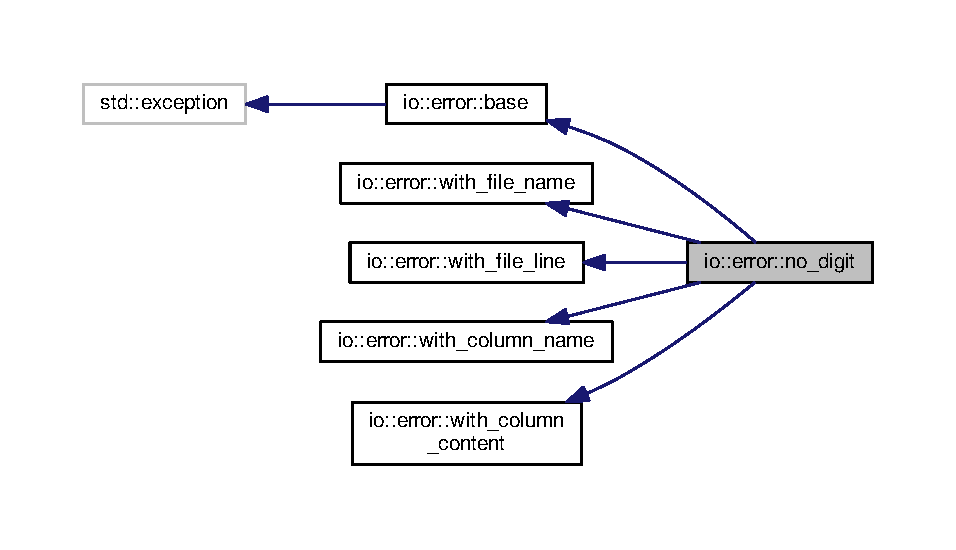
\includegraphics[width=350pt]{structio_1_1error_1_1no__digit__inherit__graph}
\end{center}
\end{figure}


Collaboration diagram for io\+:\+:error\+:\+:no\+\_\+digit\+:\nopagebreak
\begin{figure}[H]
\begin{center}
\leavevmode
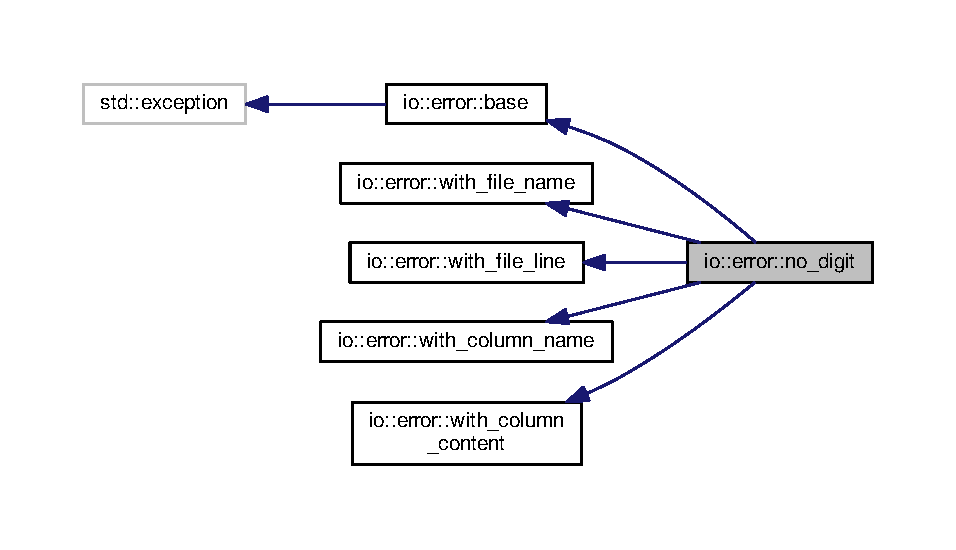
\includegraphics[width=350pt]{structio_1_1error_1_1no__digit__coll__graph}
\end{center}
\end{figure}
\subsection*{Public Member Functions}
\begin{DoxyCompactItemize}
\item 
void {\bfseries format\+\_\+error\+\_\+message} () const \label{structio_1_1error_1_1no__digit_a0e2c7f649820beb68b92dab16049388d}

\end{DoxyCompactItemize}
\subsection*{Additional Inherited Members}


The documentation for this struct was generated from the following file\+:\begin{DoxyCompactItemize}
\item 
csv.\+h\end{DoxyCompactItemize}

\section{io\+:\+:no\+\_\+quote\+\_\+escape$<$ sep $>$ Struct Template Reference}
\label{structio_1_1no__quote__escape}\index{io\+::no\+\_\+quote\+\_\+escape$<$ sep $>$@{io\+::no\+\_\+quote\+\_\+escape$<$ sep $>$}}
\subsection*{Static Public Member Functions}
\begin{DoxyCompactItemize}
\item 
static const char $\ast$ {\bfseries find\+\_\+next\+\_\+column\+\_\+end} (const char $\ast$col\+\_\+begin)\label{structio_1_1no__quote__escape_add17b043bb89445079a0448026ce86d0}

\item 
static void {\bfseries unescape} (char $\ast$\&, char $\ast$\&)\label{structio_1_1no__quote__escape_af1c217f2c995d178a91c58235191b052}

\end{DoxyCompactItemize}


The documentation for this struct was generated from the following file\+:\begin{DoxyCompactItemize}
\item 
csv.\+h\end{DoxyCompactItemize}

\section{io\+:\+:detail\+:\+:Non\+Owning\+I\+Stream\+Byte\+Source Class Reference}
\label{classio_1_1detail_1_1_non_owning_i_stream_byte_source}\index{io\+::detail\+::\+Non\+Owning\+I\+Stream\+Byte\+Source@{io\+::detail\+::\+Non\+Owning\+I\+Stream\+Byte\+Source}}


Inheritance diagram for io\+:\+:detail\+:\+:Non\+Owning\+I\+Stream\+Byte\+Source\+:\nopagebreak
\begin{figure}[H]
\begin{center}
\leavevmode
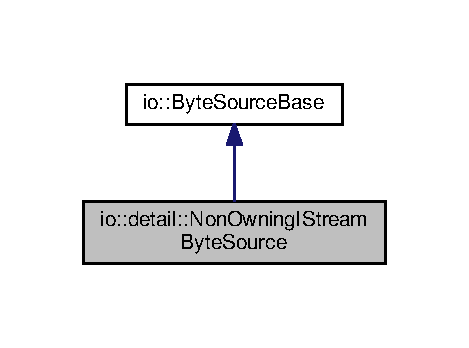
\includegraphics[width=225pt]{classio_1_1detail_1_1_non_owning_i_stream_byte_source__inherit__graph}
\end{center}
\end{figure}


Collaboration diagram for io\+:\+:detail\+:\+:Non\+Owning\+I\+Stream\+Byte\+Source\+:\nopagebreak
\begin{figure}[H]
\begin{center}
\leavevmode
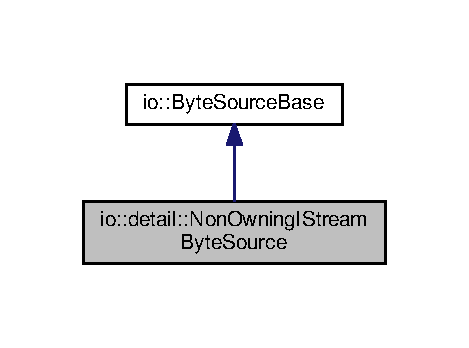
\includegraphics[width=225pt]{classio_1_1detail_1_1_non_owning_i_stream_byte_source__coll__graph}
\end{center}
\end{figure}
\subsection*{Public Member Functions}
\begin{DoxyCompactItemize}
\item 
{\bfseries Non\+Owning\+I\+Stream\+Byte\+Source} (std\+::istream \&in)\label{classio_1_1detail_1_1_non_owning_i_stream_byte_source_aacb55ba2f52ba1c30810697d6aa92169}

\item 
int {\bfseries read} (char $\ast$buffer, int size)\label{classio_1_1detail_1_1_non_owning_i_stream_byte_source_ac7b1968c8314896d7ec0ebb97fdda30d}

\end{DoxyCompactItemize}


The documentation for this class was generated from the following file\+:\begin{DoxyCompactItemize}
\item 
csv.\+h\end{DoxyCompactItemize}

\section{io\+:\+:detail\+:\+:Non\+Owning\+String\+Byte\+Source Class Reference}
\label{classio_1_1detail_1_1_non_owning_string_byte_source}\index{io\+::detail\+::\+Non\+Owning\+String\+Byte\+Source@{io\+::detail\+::\+Non\+Owning\+String\+Byte\+Source}}


Inheritance diagram for io\+:\+:detail\+:\+:Non\+Owning\+String\+Byte\+Source\+:\nopagebreak
\begin{figure}[H]
\begin{center}
\leavevmode
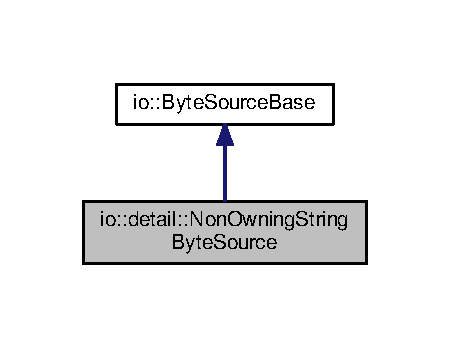
\includegraphics[width=216pt]{classio_1_1detail_1_1_non_owning_string_byte_source__inherit__graph}
\end{center}
\end{figure}


Collaboration diagram for io\+:\+:detail\+:\+:Non\+Owning\+String\+Byte\+Source\+:\nopagebreak
\begin{figure}[H]
\begin{center}
\leavevmode
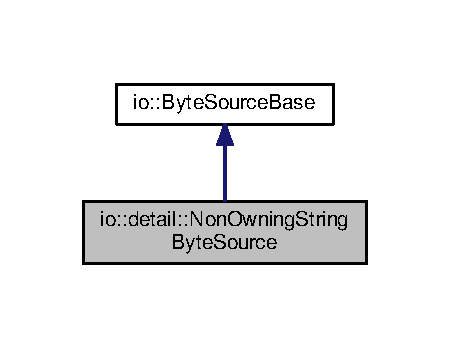
\includegraphics[width=216pt]{classio_1_1detail_1_1_non_owning_string_byte_source__coll__graph}
\end{center}
\end{figure}
\subsection*{Public Member Functions}
\begin{DoxyCompactItemize}
\item 
{\bfseries Non\+Owning\+String\+Byte\+Source} (const char $\ast$str, long long size)\label{classio_1_1detail_1_1_non_owning_string_byte_source_a8fd604017b38e20f90386b6e10bd95a3}

\item 
int {\bfseries read} (char $\ast$buffer, int desired\+\_\+byte\+\_\+count)\label{classio_1_1detail_1_1_non_owning_string_byte_source_aba194be7e3a141f40d683db483a620bb}

\end{DoxyCompactItemize}


The documentation for this class was generated from the following file\+:\begin{DoxyCompactItemize}
\item 
csv.\+h\end{DoxyCompactItemize}

\section{io\+:\+:detail\+:\+:Owning\+Std\+I\+O\+Byte\+Source\+Base Class Reference}
\label{classio_1_1detail_1_1_owning_std_i_o_byte_source_base}\index{io\+::detail\+::\+Owning\+Std\+I\+O\+Byte\+Source\+Base@{io\+::detail\+::\+Owning\+Std\+I\+O\+Byte\+Source\+Base}}


Inheritance diagram for io\+:\+:detail\+:\+:Owning\+Std\+I\+O\+Byte\+Source\+Base\+:\nopagebreak
\begin{figure}[H]
\begin{center}
\leavevmode
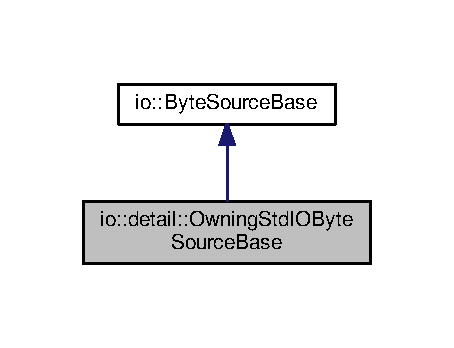
\includegraphics[width=218pt]{classio_1_1detail_1_1_owning_std_i_o_byte_source_base__inherit__graph}
\end{center}
\end{figure}


Collaboration diagram for io\+:\+:detail\+:\+:Owning\+Std\+I\+O\+Byte\+Source\+Base\+:\nopagebreak
\begin{figure}[H]
\begin{center}
\leavevmode
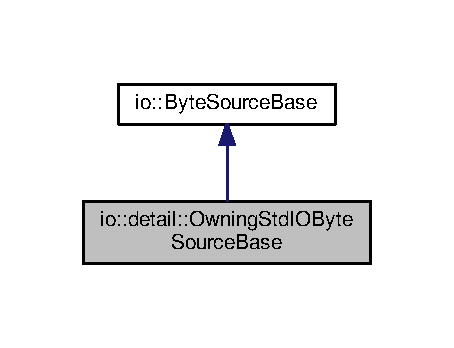
\includegraphics[width=218pt]{classio_1_1detail_1_1_owning_std_i_o_byte_source_base__coll__graph}
\end{center}
\end{figure}
\subsection*{Public Member Functions}
\begin{DoxyCompactItemize}
\item 
{\bfseries Owning\+Std\+I\+O\+Byte\+Source\+Base} (F\+I\+LE $\ast$file)\label{classio_1_1detail_1_1_owning_std_i_o_byte_source_base_a259f77d1a3c57720b54b88d9f8a3c018}

\item 
int {\bfseries read} (char $\ast$buffer, int size)\label{classio_1_1detail_1_1_owning_std_i_o_byte_source_base_a9269e7bfd07ebf2fa3518912fe7bebd0}

\end{DoxyCompactItemize}


The documentation for this class was generated from the following file\+:\begin{DoxyCompactItemize}
\item 
csv.\+h\end{DoxyCompactItemize}

\section{Page Class Reference}
\label{class_page}\index{Page@{Page}}


Collaboration diagram for Page\+:\nopagebreak
\begin{figure}[H]
\begin{center}
\leavevmode
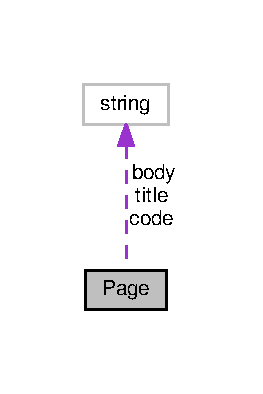
\includegraphics[width=126pt]{class_page__coll__graph}
\end{center}
\end{figure}
\subsection*{Public Member Functions}
\begin{DoxyCompactItemize}
\item 
{\bf Page} (int, std\+::string, std\+::string, std\+::string)
\begin{DoxyCompactList}\small\item\em \doxyref{Page\+::\+Page}{p.}{class_page_a426ed36ede7300b9e71bc273de894d50}. \end{DoxyCompactList}\item 
void {\bf page\+Set} (int \&, std\+::string \&, std\+::string \&, std\+::string \&)
\begin{DoxyCompactList}\small\item\em \doxyref{Page\+::page\+Set}{p.}{class_page_a09b531e0164024d9521b2cce369e73ca}. \end{DoxyCompactList}\end{DoxyCompactItemize}
\subsection*{Public Attributes}
\begin{DoxyCompactItemize}
\item 
int {\bfseries Id} = -\/1\label{class_page_a7cb1dc7c8b1cb5cbafdefee4d9292408}

\item 
float {\bfseries owner\+Id} = -\/1\label{class_page_a6e2827089066ab8b0fa8d14159521bcd}

\item 
float {\bfseries score} = -\/1\label{class_page_a29c03e7f14b2d488314dad98ea5e3fb4}

\item 
std\+::string {\bfseries title}\label{class_page_aa91345488f39e9592ab3b411f42e1db5}

\item 
std\+::string {\bfseries body}\label{class_page_a3b0083a659833f396cb804cdd043b887}

\item 
std\+::string {\bfseries code}\label{class_page_adab541347a37a237bca495eba7fe2a46}

\end{DoxyCompactItemize}


\subsection{Constructor \& Destructor Documentation}
\index{Page@{Page}!Page@{Page}}
\index{Page@{Page}!Page@{Page}}
\subsubsection[{Page(int, std\+::string, std\+::string, std\+::string)}]{\setlength{\rightskip}{0pt plus 5cm}Page\+::\+Page (
\begin{DoxyParamCaption}
\item[{int}]{i, }
\item[{std\+::string}]{t, }
\item[{std\+::string}]{b, }
\item[{std\+::string}]{c}
\end{DoxyParamCaption}
)}\label{class_page_a426ed36ede7300b9e71bc273de894d50}


\doxyref{Page\+::\+Page}{p.}{class_page_a426ed36ede7300b9e71bc273de894d50}. 


\begin{DoxyParams}{Parameters}
{\em i} & \\
\hline
{\em t} & \\
\hline
{\em b} & \\
\hline
{\em c} & Constructor for \doxyref{Page}{p.}{class_page} with values \\
\hline
\end{DoxyParams}


Here is the call graph for this function\+:\nopagebreak
\begin{figure}[H]
\begin{center}
\leavevmode
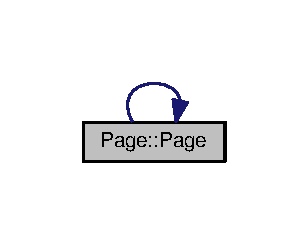
\includegraphics[width=148pt]{class_page_a426ed36ede7300b9e71bc273de894d50_cgraph}
\end{center}
\end{figure}




Here is the caller graph for this function\+:\nopagebreak
\begin{figure}[H]
\begin{center}
\leavevmode
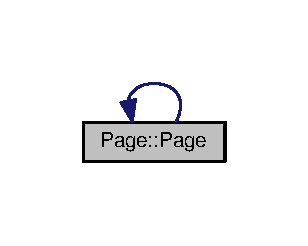
\includegraphics[width=148pt]{class_page_a426ed36ede7300b9e71bc273de894d50_icgraph}
\end{center}
\end{figure}




\subsection{Member Function Documentation}
\index{Page@{Page}!page\+Set@{page\+Set}}
\index{page\+Set@{page\+Set}!Page@{Page}}
\subsubsection[{page\+Set(int \&, std\+::string \&, std\+::string \&, std\+::string \&)}]{\setlength{\rightskip}{0pt plus 5cm}void Page\+::page\+Set (
\begin{DoxyParamCaption}
\item[{int \&}]{i, }
\item[{std\+::string \&}]{t, }
\item[{std\+::string \&}]{b, }
\item[{std\+::string \&}]{c}
\end{DoxyParamCaption}
)}\label{class_page_a09b531e0164024d9521b2cce369e73ca}


\doxyref{Page\+::page\+Set}{p.}{class_page_a09b531e0164024d9521b2cce369e73ca}. 


\begin{DoxyParams}{Parameters}
{\em i} & \\
\hline
{\em t} & \\
\hline
{\em b} & \\
\hline
{\em c} & Sets all values for pages \\
\hline
\end{DoxyParams}


The documentation for this class was generated from the following files\+:\begin{DoxyCompactItemize}
\item 
page.\+h\item 
page.\+cpp\end{DoxyCompactItemize}

\section{Parser Class Reference}
\label{class_parser}\index{Parser@{Parser}}


Collaboration diagram for Parser\+:\nopagebreak
\begin{figure}[H]
\begin{center}
\leavevmode
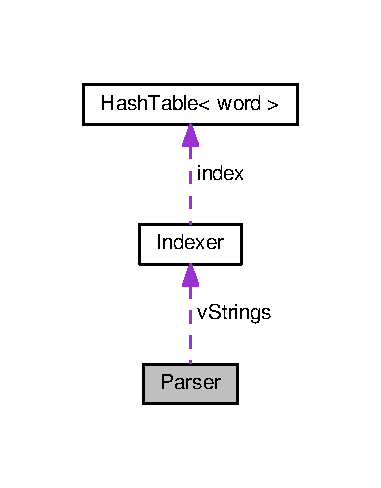
\includegraphics[width=183pt]{class_parser__coll__graph}
\end{center}
\end{figure}
\subsection*{Public Member Functions}
\begin{DoxyCompactItemize}
\item 
{\bf Parser} ()\label{class_parser_a12234f6cd36b61af4b50c94a179422c1}

\begin{DoxyCompactList}\small\item\em \doxyref{Parser\+::\+Parser}{p.}{class_parser_a12234f6cd36b61af4b50c94a179422c1} Fills rows of entire questions with a filler/empty object. \end{DoxyCompactList}\item 
{\bfseries Parser} (char $\ast$, char $\ast$)\label{class_parser_a0b74f3568fde911fab6b7826b4cdaa30}

\item 
int {\bf read\+File} (char $\ast$)
\begin{DoxyCompactList}\small\item\em \doxyref{Parser\+::read\+File}{p.}{class_parser_a9a4c8a2d713a3f555b0829aa076bfce3}. \end{DoxyCompactList}\item 
void {\bf read\+Tag\+File} (char $\ast$)
\begin{DoxyCompactList}\small\item\em \doxyref{Parser\+::read\+Tag\+File}{p.}{class_parser_a60187c7fdef5329fd84774204468d3ad}. \end{DoxyCompactList}\item 
int {\bfseries read\+Id} (int)\label{class_parser_a446505f72b33249f61adef9c642e769a}

\item 
int {\bfseries read\+Score} (int)\label{class_parser_a222dd63736adc8b64f6d5e8cd443a10d}

\item 
int {\bfseries read\+Tag\+Id} (int)\label{class_parser_ad279e4d18624c84df8a540f64ced8cb6}

\item 
string {\bfseries read\+Title} (int)\label{class_parser_adb2a91073f53b7dcc332ee4082629933}

\item 
string {\bfseries read\+Body} (int)\label{class_parser_abf57cc6c1dc7d7ecdf45a8c79eb65771}

\item 
string {\bfseries read\+Code} (int)\label{class_parser_a10713d4bb2867dd82a5f47e8ac823336}

\item 
int {\bfseries Total\+Questions} ()\label{class_parser_a8daf26c7d4bae0eb778f3426b94e3d86}

\item 
int {\bf find\+File} (int)
\begin{DoxyCompactList}\small\item\em \doxyref{Parser\+::find\+File}{p.}{class_parser_a103eea4c90c36e5c0fd9c55232565ded}. \end{DoxyCompactList}\item 
void {\bf clear} ()\label{class_parser_abb54cb3c787646ed220d8faee2af5e15}

\begin{DoxyCompactList}\small\item\em \doxyref{Parser\+::clear}{p.}{class_parser_abb54cb3c787646ed220d8faee2af5e15} Clears all Entries. \end{DoxyCompactList}\end{DoxyCompactItemize}
\subsection*{Public Attributes}
\begin{DoxyCompactItemize}
\item 
int {\bfseries doc\+Load\+Pos} = 0\label{class_parser_a16150bbf6d2c5f2d30ec1362bb809853}

\item 
{\bf Indexer} $\ast$ {\bfseries v\+Strings} = new {\bf Indexer}()\label{class_parser_abed69bdba05da4901492c726439f7bd1}

\end{DoxyCompactItemize}


\subsection{Member Function Documentation}
\index{Parser@{Parser}!find\+File@{find\+File}}
\index{find\+File@{find\+File}!Parser@{Parser}}
\subsubsection[{find\+File(int)}]{\setlength{\rightskip}{0pt plus 5cm}int Parser\+::find\+File (
\begin{DoxyParamCaption}
\item[{int}]{ID}
\end{DoxyParamCaption}
)}\label{class_parser_a103eea4c90c36e5c0fd9c55232565ded}


\doxyref{Parser\+::find\+File}{p.}{class_parser_a103eea4c90c36e5c0fd9c55232565ded}. 


\begin{DoxyParams}{Parameters}
{\em ID} & \\
\hline
\end{DoxyParams}
\begin{DoxyReturn}{Returns}
Finds and returns file location based on index in id\+Locations vector 
\end{DoxyReturn}


Here is the call graph for this function\+:\nopagebreak
\begin{figure}[H]
\begin{center}
\leavevmode
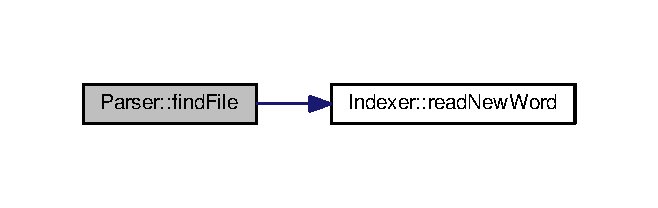
\includegraphics[width=316pt]{class_parser_a103eea4c90c36e5c0fd9c55232565ded_cgraph}
\end{center}
\end{figure}


\index{Parser@{Parser}!read\+File@{read\+File}}
\index{read\+File@{read\+File}!Parser@{Parser}}
\subsubsection[{read\+File(char $\ast$)}]{\setlength{\rightskip}{0pt plus 5cm}void Parser\+::read\+File (
\begin{DoxyParamCaption}
\item[{char $\ast$}]{file}
\end{DoxyParamCaption}
)}\label{class_parser_a9a4c8a2d713a3f555b0829aa076bfce3}


\doxyref{Parser\+::read\+File}{p.}{class_parser_a9a4c8a2d713a3f555b0829aa076bfce3}. 


\begin{DoxyParams}{Parameters}
{\em file} & \\
\hline
\end{DoxyParams}
\begin{DoxyReturn}{Returns}
Accepts a file, reads it row by row and stores the data into \doxyref{Hash\+Table}{p.}{class_hash_table} 
\end{DoxyReturn}
\index{Parser@{Parser}!read\+Tag\+File@{read\+Tag\+File}}
\index{read\+Tag\+File@{read\+Tag\+File}!Parser@{Parser}}
\subsubsection[{read\+Tag\+File(char $\ast$)}]{\setlength{\rightskip}{0pt plus 5cm}void Parser\+::read\+Tag\+File (
\begin{DoxyParamCaption}
\item[{char $\ast$}]{file}
\end{DoxyParamCaption}
)}\label{class_parser_a60187c7fdef5329fd84774204468d3ad}


\doxyref{Parser\+::read\+Tag\+File}{p.}{class_parser_a60187c7fdef5329fd84774204468d3ad}. 


\begin{DoxyParams}{Parameters}
{\em file} & Reads in a tag file with path that is passed in \\
\hline
\end{DoxyParams}


Here is the call graph for this function\+:\nopagebreak
\begin{figure}[H]
\begin{center}
\leavevmode
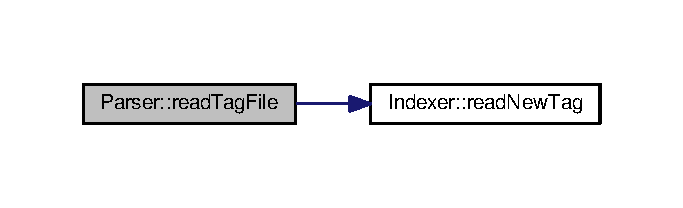
\includegraphics[width=328pt]{class_parser_a60187c7fdef5329fd84774204468d3ad_cgraph}
\end{center}
\end{figure}




The documentation for this class was generated from the following files\+:\begin{DoxyCompactItemize}
\item 
parser.\+h\item 
parser.\+cpp\item 
parser\+\_\+noncompiling.\+cpp\end{DoxyCompactItemize}

\section{query Class Reference}
\label{classquery}\index{query@{query}}
\subsection*{Public Member Functions}
\begin{DoxyCompactItemize}
\item 
{\bf query} ()\label{classquery_a362462c8a27b180a00f83f3a13b71865}

\begin{DoxyCompactList}\small\item\em \doxyref{query\+::query}{p.}{classquery_a362462c8a27b180a00f83f3a13b71865} \end{DoxyCompactList}\item 
std\+::vector$<$ {\bf q\+Word} $>$ {\bf get\+Search} ()
\begin{DoxyCompactList}\small\item\em \doxyref{query\+::get\+Search}{p.}{classquery_a88076e4a26d1ef693683c41291aec57b} \end{DoxyCompactList}\item 
void {\bf process\+Search} (std\+::string \&)
\begin{DoxyCompactList}\small\item\em \doxyref{query\+::process\+Search}{p.}{classquery_a9b5fa728a7b1e87b77cf6bced59e112a} \end{DoxyCompactList}\end{DoxyCompactItemize}
\subsection*{Public Attributes}
\begin{DoxyCompactItemize}
\item 
std\+::vector$<$ {\bf q\+Word} $>$ {\bfseries search}\label{classquery_ac45356f3253427fa80cc8668e703fb92}

\end{DoxyCompactItemize}


\subsection{Member Function Documentation}
\index{query@{query}!get\+Search@{get\+Search}}
\index{get\+Search@{get\+Search}!query@{query}}
\subsubsection[{get\+Search()}]{\setlength{\rightskip}{0pt plus 5cm}std\+::vector$<$ {\bf q\+Word} $>$ query\+::get\+Search (
\begin{DoxyParamCaption}
{}
\end{DoxyParamCaption}
)}\label{classquery_a88076e4a26d1ef693683c41291aec57b}


\doxyref{query\+::get\+Search}{p.}{classquery_a88076e4a26d1ef693683c41291aec57b} 

\begin{DoxyReturn}{Returns}
Returns vector of qwords that is set with query settings 
\end{DoxyReturn}
\index{query@{query}!process\+Search@{process\+Search}}
\index{process\+Search@{process\+Search}!query@{query}}
\subsubsection[{process\+Search(std\+::string \&)}]{\setlength{\rightskip}{0pt plus 5cm}void query\+::process\+Search (
\begin{DoxyParamCaption}
\item[{std\+::string \&}]{s}
\end{DoxyParamCaption}
)}\label{classquery_a9b5fa728a7b1e87b77cf6bced59e112a}


\doxyref{query\+::process\+Search}{p.}{classquery_a9b5fa728a7b1e87b77cf6bced59e112a} 


\begin{DoxyParams}{Parameters}
{\em s} & Processes user query and loads the values/settings into vector of q\+Words \\
\hline
\end{DoxyParams}


The documentation for this class was generated from the following files\+:\begin{DoxyCompactItemize}
\item 
query.\+h\item 
query.\+cpp\end{DoxyCompactItemize}

\section{q\+Word Class Reference}
\label{classq_word}\index{q\+Word@{q\+Word}}
\subsection*{Public Member Functions}
\begin{DoxyCompactItemize}
\item 
{\bf q\+Word} ()\label{classq_word_ae45dac4632b9d4b35abf1c520f8922db}

\begin{DoxyCompactList}\small\item\em \doxyref{q\+Word\+::q\+Word}{p.}{classq_word_ae45dac4632b9d4b35abf1c520f8922db} \end{DoxyCompactList}\item 
{\bf q\+Word} (std\+::string, bool, bool, bool)
\begin{DoxyCompactList}\small\item\em \doxyref{q\+Word\+::q\+Word}{p.}{classq_word_ae45dac4632b9d4b35abf1c520f8922db} \end{DoxyCompactList}\item 
void {\bf set\+Word} (std\+::string)
\begin{DoxyCompactList}\small\item\em \doxyref{q\+Word\+::set\+Word}{p.}{classq_word_a7350306b6c18d2fd1e684abe0f99e9d3} \end{DoxyCompactList}\item 
std\+::string {\bf get\+Word} ()
\begin{DoxyCompactList}\small\item\em \doxyref{q\+Word\+::get\+Word}{p.}{classq_word_aa2ae9e11027aea187b02d0d6fa21baf1} \end{DoxyCompactList}\item 
void {\bf set\+And} (bool)
\begin{DoxyCompactList}\small\item\em \doxyref{q\+Word\+::set\+And}{p.}{classq_word_a47df73f675137e13686b89e1be109fd0} \end{DoxyCompactList}\item 
bool {\bf get\+And} ()
\begin{DoxyCompactList}\small\item\em \doxyref{q\+Word\+::get\+And}{p.}{classq_word_adceb37ae55c0081d2250bb9dc89a4682} \end{DoxyCompactList}\item 
void {\bf set\+Or} (bool)
\begin{DoxyCompactList}\small\item\em \doxyref{q\+Word\+::set\+Or}{p.}{classq_word_a6e11fbf7bd0a2e78bdf7b31231a86f39} \end{DoxyCompactList}\item 
bool {\bf get\+Or} ()
\begin{DoxyCompactList}\small\item\em \doxyref{q\+Word\+::get\+Or}{p.}{classq_word_ab8145659960d25eaf4f7a60d7aeca77a} \end{DoxyCompactList}\item 
void {\bf set\+Not} (bool)
\begin{DoxyCompactList}\small\item\em \doxyref{q\+Word\+::set\+Not}{p.}{classq_word_adfe93a34545c407758affb0ec1ab7624} \end{DoxyCompactList}\item 
bool {\bf get\+Not} ()
\begin{DoxyCompactList}\small\item\em \doxyref{q\+Word\+::get\+Not}{p.}{classq_word_a30655704a3bd9fdcb7bd5de62c0dec9c} \end{DoxyCompactList}\end{DoxyCompactItemize}


\subsection{Constructor \& Destructor Documentation}
\index{q\+Word@{q\+Word}!q\+Word@{q\+Word}}
\index{q\+Word@{q\+Word}!q\+Word@{q\+Word}}
\subsubsection[{q\+Word(std\+::string, bool, bool, bool)}]{\setlength{\rightskip}{0pt plus 5cm}q\+Word\+::q\+Word (
\begin{DoxyParamCaption}
\item[{std\+::string}]{word, }
\item[{bool}]{a, }
\item[{bool}]{o, }
\item[{bool}]{n}
\end{DoxyParamCaption}
)}\label{classq_word_a12673cacfa8cc4deb08c184d346e7ad2}


\doxyref{q\+Word\+::q\+Word}{p.}{classq_word_ae45dac4632b9d4b35abf1c520f8922db} 


\begin{DoxyParams}{Parameters}
{\em word} & \\
\hline
{\em a} & \\
\hline
{\em o} & \\
\hline
{\em n} & Contructor that sets \doxyref{q\+Word}{p.}{classq_word} values that are set \\
\hline
\end{DoxyParams}


\subsection{Member Function Documentation}
\index{q\+Word@{q\+Word}!get\+And@{get\+And}}
\index{get\+And@{get\+And}!q\+Word@{q\+Word}}
\subsubsection[{get\+And()}]{\setlength{\rightskip}{0pt plus 5cm}bool q\+Word\+::get\+And (
\begin{DoxyParamCaption}
{}
\end{DoxyParamCaption}
)}\label{classq_word_adceb37ae55c0081d2250bb9dc89a4682}


\doxyref{q\+Word\+::get\+And}{p.}{classq_word_adceb37ae55c0081d2250bb9dc89a4682} 

\begin{DoxyReturn}{Returns}

\end{DoxyReturn}
\index{q\+Word@{q\+Word}!get\+Not@{get\+Not}}
\index{get\+Not@{get\+Not}!q\+Word@{q\+Word}}
\subsubsection[{get\+Not()}]{\setlength{\rightskip}{0pt plus 5cm}bool q\+Word\+::get\+Not (
\begin{DoxyParamCaption}
{}
\end{DoxyParamCaption}
)}\label{classq_word_a30655704a3bd9fdcb7bd5de62c0dec9c}


\doxyref{q\+Word\+::get\+Not}{p.}{classq_word_a30655704a3bd9fdcb7bd5de62c0dec9c} 

\begin{DoxyReturn}{Returns}

\end{DoxyReturn}
\index{q\+Word@{q\+Word}!get\+Or@{get\+Or}}
\index{get\+Or@{get\+Or}!q\+Word@{q\+Word}}
\subsubsection[{get\+Or()}]{\setlength{\rightskip}{0pt plus 5cm}bool q\+Word\+::get\+Or (
\begin{DoxyParamCaption}
{}
\end{DoxyParamCaption}
)}\label{classq_word_ab8145659960d25eaf4f7a60d7aeca77a}


\doxyref{q\+Word\+::get\+Or}{p.}{classq_word_ab8145659960d25eaf4f7a60d7aeca77a} 

\begin{DoxyReturn}{Returns}

\end{DoxyReturn}
\index{q\+Word@{q\+Word}!get\+Word@{get\+Word}}
\index{get\+Word@{get\+Word}!q\+Word@{q\+Word}}
\subsubsection[{get\+Word()}]{\setlength{\rightskip}{0pt plus 5cm}std\+::string q\+Word\+::get\+Word (
\begin{DoxyParamCaption}
{}
\end{DoxyParamCaption}
)}\label{classq_word_aa2ae9e11027aea187b02d0d6fa21baf1}


\doxyref{q\+Word\+::get\+Word}{p.}{classq_word_aa2ae9e11027aea187b02d0d6fa21baf1} 

\begin{DoxyReturn}{Returns}

\end{DoxyReturn}
\index{q\+Word@{q\+Word}!set\+And@{set\+And}}
\index{set\+And@{set\+And}!q\+Word@{q\+Word}}
\subsubsection[{set\+And(bool)}]{\setlength{\rightskip}{0pt plus 5cm}void q\+Word\+::set\+And (
\begin{DoxyParamCaption}
\item[{bool}]{a}
\end{DoxyParamCaption}
)}\label{classq_word_a47df73f675137e13686b89e1be109fd0}


\doxyref{q\+Word\+::set\+And}{p.}{classq_word_a47df73f675137e13686b89e1be109fd0} 


\begin{DoxyParams}{Parameters}
{\em a} & \\
\hline
\end{DoxyParams}
\index{q\+Word@{q\+Word}!set\+Not@{set\+Not}}
\index{set\+Not@{set\+Not}!q\+Word@{q\+Word}}
\subsubsection[{set\+Not(bool)}]{\setlength{\rightskip}{0pt plus 5cm}void q\+Word\+::set\+Not (
\begin{DoxyParamCaption}
\item[{bool}]{n}
\end{DoxyParamCaption}
)}\label{classq_word_adfe93a34545c407758affb0ec1ab7624}


\doxyref{q\+Word\+::set\+Not}{p.}{classq_word_adfe93a34545c407758affb0ec1ab7624} 


\begin{DoxyParams}{Parameters}
{\em n} & \\
\hline
\end{DoxyParams}
\index{q\+Word@{q\+Word}!set\+Or@{set\+Or}}
\index{set\+Or@{set\+Or}!q\+Word@{q\+Word}}
\subsubsection[{set\+Or(bool)}]{\setlength{\rightskip}{0pt plus 5cm}void q\+Word\+::set\+Or (
\begin{DoxyParamCaption}
\item[{bool}]{o}
\end{DoxyParamCaption}
)}\label{classq_word_a6e11fbf7bd0a2e78bdf7b31231a86f39}


\doxyref{q\+Word\+::set\+Or}{p.}{classq_word_a6e11fbf7bd0a2e78bdf7b31231a86f39} 


\begin{DoxyParams}{Parameters}
{\em o} & \\
\hline
\end{DoxyParams}
\index{q\+Word@{q\+Word}!set\+Word@{set\+Word}}
\index{set\+Word@{set\+Word}!q\+Word@{q\+Word}}
\subsubsection[{set\+Word(std\+::string)}]{\setlength{\rightskip}{0pt plus 5cm}void q\+Word\+::set\+Word (
\begin{DoxyParamCaption}
\item[{std\+::string}]{word}
\end{DoxyParamCaption}
)}\label{classq_word_a7350306b6c18d2fd1e684abe0f99e9d3}


\doxyref{q\+Word\+::set\+Word}{p.}{classq_word_a7350306b6c18d2fd1e684abe0f99e9d3} 


\begin{DoxyParams}{Parameters}
{\em word} & \\
\hline
\end{DoxyParams}


The documentation for this class was generated from the following files\+:\begin{DoxyCompactItemize}
\item 
qword.\+h\item 
qword.\+cpp\end{DoxyCompactItemize}

\section{result Class Reference}
\label{classresult}\index{result@{result}}


Collaboration diagram for result\+:\nopagebreak
\begin{figure}[H]
\begin{center}
\leavevmode
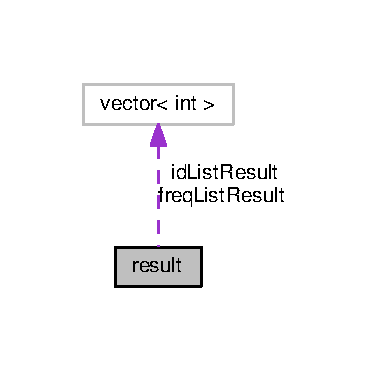
\includegraphics[width=177pt]{classresult__coll__graph}
\end{center}
\end{figure}
\subsection*{Public Member Functions}
\begin{DoxyCompactItemize}
\item 
{\bf result} ()\label{classresult_ad82f937012d03ea93364031666897225}

\begin{DoxyCompactList}\small\item\em result \end{DoxyCompactList}\item 
{\bf result} (vector$<$ {\bf q\+Word} $>$ \&temp1, {\bf Parser} $\ast$\&p)
\begin{DoxyCompactList}\small\item\em result \end{DoxyCompactList}\item 
void {\bf merge\+And} (vector$<$ int $>$ \&id\+Merge, vector$<$ int $>$ \&freq\+Merge)
\begin{DoxyCompactList}\small\item\em merge\+And \end{DoxyCompactList}\item 
void {\bf merge\+Or} (vector$<$ int $>$ \&id\+Merge, vector$<$ int $>$ \&freq\+Merge)
\begin{DoxyCompactList}\small\item\em merge\+Or \end{DoxyCompactList}\item 
void {\bf merge\+Not} (vector$<$ int $>$ \&id\+Merge, vector$<$ int $>$ \&freq\+Merge)
\begin{DoxyCompactList}\small\item\em merge\+Not \end{DoxyCompactList}\item 
void {\bf print} ()\label{classresult_aa3017b87fb7e7a65365cc9575731047b}

\begin{DoxyCompactList}\small\item\em print Prints all word values that are sorted by frequency \end{DoxyCompactList}\item 
void {\bf q\+Sort} (int left, int right)
\begin{DoxyCompactList}\small\item\em q\+Sort \end{DoxyCompactList}\item 
void {\bfseries q\+Sort} ()\label{classresult_a68389b354f9d9020bfa51267b8cd9233}

\end{DoxyCompactItemize}
\subsection*{Public Attributes}
\begin{DoxyCompactItemize}
\item 
vector$<$ int $>$ {\bfseries id\+List\+Result}\label{classresult_a133d56a418a980dabb34659f27d4f0ad}

\item 
vector$<$ int $>$ {\bfseries freq\+List\+Result}\label{classresult_a2a95dd4c44436b666244746e1527e8bf}

\end{DoxyCompactItemize}


\subsection{Constructor \& Destructor Documentation}
\index{result@{result}!result@{result}}
\index{result@{result}!result@{result}}
\subsubsection[{result(vector$<$ q\+Word $>$ \&temp1, Parser $\ast$\&p)}]{\setlength{\rightskip}{0pt plus 5cm}result\+::result (
\begin{DoxyParamCaption}
\item[{vector$<$ {\bf q\+Word} $>$ \&}]{temp1, }
\item[{{\bf Parser} $\ast$\&}]{p}
\end{DoxyParamCaption}
)\hspace{0.3cm}{\ttfamily [inline]}}\label{classresult_ad9ce0309cd3634bfecabd4c121cc7036}


result 


\begin{DoxyParams}{Parameters}
{\em temp1} & \\
\hline
{\em p} & Merges/sorts/updates frequencies based on query bool values \\
\hline
\end{DoxyParams}


Here is the call graph for this function\+:\nopagebreak
\begin{figure}[H]
\begin{center}
\leavevmode
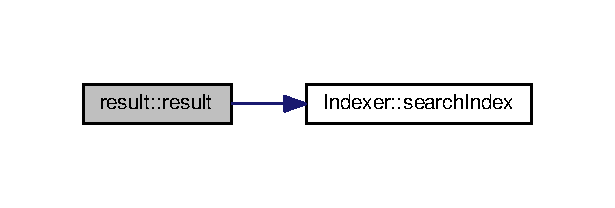
\includegraphics[width=295pt]{classresult_ad9ce0309cd3634bfecabd4c121cc7036_cgraph}
\end{center}
\end{figure}




\subsection{Member Function Documentation}
\index{result@{result}!merge\+And@{merge\+And}}
\index{merge\+And@{merge\+And}!result@{result}}
\subsubsection[{merge\+And(vector$<$ int $>$ \&id\+Merge, vector$<$ int $>$ \&freq\+Merge)}]{\setlength{\rightskip}{0pt plus 5cm}void result\+::merge\+And (
\begin{DoxyParamCaption}
\item[{vector$<$ int $>$ \&}]{id\+Merge, }
\item[{vector$<$ int $>$ \&}]{freq\+Merge}
\end{DoxyParamCaption}
)\hspace{0.3cm}{\ttfamily [inline]}}\label{classresult_aa3698ce540402c3c7e018359a83c4360}


merge\+And 


\begin{DoxyParams}{Parameters}
{\em id\+Merge} & \\
\hline
{\em freq\+Merge} & Merges ID and Frequency with A\+ND based on query bool values \\
\hline
\end{DoxyParams}
\index{result@{result}!merge\+Not@{merge\+Not}}
\index{merge\+Not@{merge\+Not}!result@{result}}
\subsubsection[{merge\+Not(vector$<$ int $>$ \&id\+Merge, vector$<$ int $>$ \&freq\+Merge)}]{\setlength{\rightskip}{0pt plus 5cm}void result\+::merge\+Not (
\begin{DoxyParamCaption}
\item[{vector$<$ int $>$ \&}]{id\+Merge, }
\item[{vector$<$ int $>$ \&}]{freq\+Merge}
\end{DoxyParamCaption}
)\hspace{0.3cm}{\ttfamily [inline]}}\label{classresult_ae8e1c308f6cc22759fbaced1df59b571}


merge\+Not 


\begin{DoxyParams}{Parameters}
{\em id\+Merge} & \\
\hline
{\em freq\+Merge} & Merges ID and Frequency with N\+OT based on query bool values \\
\hline
\end{DoxyParams}
\index{result@{result}!merge\+Or@{merge\+Or}}
\index{merge\+Or@{merge\+Or}!result@{result}}
\subsubsection[{merge\+Or(vector$<$ int $>$ \&id\+Merge, vector$<$ int $>$ \&freq\+Merge)}]{\setlength{\rightskip}{0pt plus 5cm}void result\+::merge\+Or (
\begin{DoxyParamCaption}
\item[{vector$<$ int $>$ \&}]{id\+Merge, }
\item[{vector$<$ int $>$ \&}]{freq\+Merge}
\end{DoxyParamCaption}
)\hspace{0.3cm}{\ttfamily [inline]}}\label{classresult_a5176b5c535444a8877863953c265ea29}


merge\+Or 


\begin{DoxyParams}{Parameters}
{\em id\+Merge} & \\
\hline
{\em freq\+Merge} & Merges ID and Frequency with OR based on query bool values \\
\hline
\end{DoxyParams}
\index{result@{result}!q\+Sort@{q\+Sort}}
\index{q\+Sort@{q\+Sort}!result@{result}}
\subsubsection[{q\+Sort(int left, int right)}]{\setlength{\rightskip}{0pt plus 5cm}void result\+::q\+Sort (
\begin{DoxyParamCaption}
\item[{int}]{left, }
\item[{int}]{right}
\end{DoxyParamCaption}
)\hspace{0.3cm}{\ttfamily [inline]}}\label{classresult_accfe13319340168b32ac5f41ab2d7a9f}


q\+Sort 


\begin{DoxyParams}{Parameters}
{\em left} & \\
\hline
{\em right} & Sorting functions for relevancy rankings Uses Sprint 3 algorithm for sorting vectors (In D\+S\+Vector) \\
\hline
\end{DoxyParams}


The documentation for this class was generated from the following file\+:\begin{DoxyCompactItemize}
\item 
result.\+h\end{DoxyCompactItemize}

\section{io\+:\+:set\+\_\+to\+\_\+max\+\_\+on\+\_\+overflow Struct Reference}
\label{structio_1_1set__to__max__on__overflow}\index{io\+::set\+\_\+to\+\_\+max\+\_\+on\+\_\+overflow@{io\+::set\+\_\+to\+\_\+max\+\_\+on\+\_\+overflow}}
\subsection*{Static Public Member Functions}
\begin{DoxyCompactItemize}
\item 
{\footnotesize template$<$class T $>$ }\\static void {\bfseries on\+\_\+overflow} (T \&x)\label{structio_1_1set__to__max__on__overflow_a770dee97a1ee55131163e6be8d4c0d9d}

\item 
{\footnotesize template$<$class T $>$ }\\static void {\bfseries on\+\_\+underflow} (T \&x)\label{structio_1_1set__to__max__on__overflow_a812d316e2b23247df19ca83bfda90a59}

\end{DoxyCompactItemize}


The documentation for this struct was generated from the following file\+:\begin{DoxyCompactItemize}
\item 
csv.\+h\end{DoxyCompactItemize}

\section{io\+:\+:single\+\_\+and\+\_\+empty\+\_\+line\+\_\+comment$<$ comment\+\_\+start\+\_\+char\+\_\+list $>$ Struct Template Reference}
\label{structio_1_1single__and__empty__line__comment}\index{io\+::single\+\_\+and\+\_\+empty\+\_\+line\+\_\+comment$<$ comment\+\_\+start\+\_\+char\+\_\+list $>$@{io\+::single\+\_\+and\+\_\+empty\+\_\+line\+\_\+comment$<$ comment\+\_\+start\+\_\+char\+\_\+list $>$}}
\subsection*{Static Public Member Functions}
\begin{DoxyCompactItemize}
\item 
static bool {\bfseries is\+\_\+comment} (const char $\ast$line)\label{structio_1_1single__and__empty__line__comment_a93a1556dfe4d7e6e3a674d576c4b30f4}

\end{DoxyCompactItemize}


The documentation for this struct was generated from the following file\+:\begin{DoxyCompactItemize}
\item 
csv.\+h\end{DoxyCompactItemize}

\section{io\+:\+:single\+\_\+line\+\_\+comment$<$ comment\+\_\+start\+\_\+char\+\_\+list $>$ Struct Template Reference}
\label{structio_1_1single__line__comment}\index{io\+::single\+\_\+line\+\_\+comment$<$ comment\+\_\+start\+\_\+char\+\_\+list $>$@{io\+::single\+\_\+line\+\_\+comment$<$ comment\+\_\+start\+\_\+char\+\_\+list $>$}}
\subsection*{Static Public Member Functions}
\begin{DoxyCompactItemize}
\item 
static bool {\bfseries is\+\_\+comment} (const char $\ast$line)\label{structio_1_1single__line__comment_ac4b029bb0efd251505f8e610cc308a92}

\end{DoxyCompactItemize}


The documentation for this struct was generated from the following file\+:\begin{DoxyCompactItemize}
\item 
csv.\+h\end{DoxyCompactItemize}

\section{io\+:\+:detail\+:\+:Synchronous\+Reader Class Reference}
\label{classio_1_1detail_1_1_synchronous_reader}\index{io\+::detail\+::\+Synchronous\+Reader@{io\+::detail\+::\+Synchronous\+Reader}}
\subsection*{Public Member Functions}
\begin{DoxyCompactItemize}
\item 
void {\bfseries init} (std\+::unique\+\_\+ptr$<$ {\bf Byte\+Source\+Base} $>$arg\+\_\+byte\+\_\+source)\label{classio_1_1detail_1_1_synchronous_reader_a4dc78563ff667b92ad3096a94e834eb5}

\item 
bool {\bfseries is\+\_\+valid} () const \label{classio_1_1detail_1_1_synchronous_reader_a963aaeed2b0a1177e16b88df61cab948}

\item 
void {\bfseries start\+\_\+read} (char $\ast$arg\+\_\+buffer, int arg\+\_\+desired\+\_\+byte\+\_\+count)\label{classio_1_1detail_1_1_synchronous_reader_a6cad1371b97e14f660914898b16433c4}

\item 
int {\bfseries finish\+\_\+read} ()\label{classio_1_1detail_1_1_synchronous_reader_a519a0cb25c641d2e51b6542749c44606}

\end{DoxyCompactItemize}


The documentation for this class was generated from the following file\+:\begin{DoxyCompactItemize}
\item 
csv.\+h\end{DoxyCompactItemize}

\section{Tag Class Reference}
\label{class_tag}\index{Tag@{Tag}}


Collaboration diagram for Tag\+:\nopagebreak
\begin{figure}[H]
\begin{center}
\leavevmode
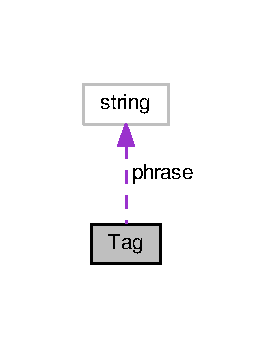
\includegraphics[width=134pt]{class_tag__coll__graph}
\end{center}
\end{figure}
\subsection*{Public Member Functions}
\begin{DoxyCompactItemize}
\item 
{\bf Tag} (float, std\+::string)
\begin{DoxyCompactList}\small\item\em \doxyref{Tag\+::\+Tag}{p.}{class_tag_ae81764cc0fef95018cc3d2f4099ff17a}. \end{DoxyCompactList}\item 
{\bf Tag} ()\label{class_tag_af2008705aa18e21efecb9e737b6b1a26}

\begin{DoxyCompactList}\small\item\em \doxyref{Tag\+::\+Tag}{p.}{class_tag_ae81764cc0fef95018cc3d2f4099ff17a}. \end{DoxyCompactList}\item 
void {\bf set\+Tag\+Id} (float)
\begin{DoxyCompactList}\small\item\em \doxyref{Tag\+::set\+Tag\+Id}{p.}{class_tag_a08718a6db6985cf4231200cd80d7f154}. \end{DoxyCompactList}\item 
void {\bf set\+Tag} (std\+::string)
\begin{DoxyCompactList}\small\item\em \doxyref{Tag\+::set\+Tag}{p.}{class_tag_a2b36dc24eb0aade1c074eae9b14c804f}. \end{DoxyCompactList}\end{DoxyCompactItemize}
\subsection*{Public Attributes}
\begin{DoxyCompactItemize}
\item 
float {\bfseries tag\+Id} = -\/1\label{class_tag_a0819b891f6f97661cb7ab1611fcd7623}

\item 
std\+::string {\bfseries phrase} = \char`\"{} \char`\"{}\label{class_tag_ad452a55e8b3e1e70af85330e8ca20349}

\end{DoxyCompactItemize}


\subsection{Constructor \& Destructor Documentation}
\index{Tag@{Tag}!Tag@{Tag}}
\index{Tag@{Tag}!Tag@{Tag}}
\subsubsection[{Tag(float, std\+::string)}]{\setlength{\rightskip}{0pt plus 5cm}Tag\+::\+Tag (
\begin{DoxyParamCaption}
\item[{float}]{i, }
\item[{std\+::string}]{p}
\end{DoxyParamCaption}
)}\label{class_tag_ae81764cc0fef95018cc3d2f4099ff17a}


\doxyref{Tag\+::\+Tag}{p.}{class_tag_ae81764cc0fef95018cc3d2f4099ff17a}. 


\begin{DoxyParams}{Parameters}
{\em i} & \\
\hline
{\em p} & \\
\hline
\end{DoxyParams}


\subsection{Member Function Documentation}
\index{Tag@{Tag}!set\+Tag@{set\+Tag}}
\index{set\+Tag@{set\+Tag}!Tag@{Tag}}
\subsubsection[{set\+Tag(std\+::string)}]{\setlength{\rightskip}{0pt plus 5cm}void Tag\+::set\+Tag (
\begin{DoxyParamCaption}
\item[{std\+::string}]{p}
\end{DoxyParamCaption}
)}\label{class_tag_a2b36dc24eb0aade1c074eae9b14c804f}


\doxyref{Tag\+::set\+Tag}{p.}{class_tag_a2b36dc24eb0aade1c074eae9b14c804f}. 


\begin{DoxyParams}{Parameters}
{\em p} & \\
\hline
\end{DoxyParams}
\index{Tag@{Tag}!set\+Tag\+Id@{set\+Tag\+Id}}
\index{set\+Tag\+Id@{set\+Tag\+Id}!Tag@{Tag}}
\subsubsection[{set\+Tag\+Id(float)}]{\setlength{\rightskip}{0pt plus 5cm}void Tag\+::set\+Tag\+Id (
\begin{DoxyParamCaption}
\item[{float}]{i}
\end{DoxyParamCaption}
)}\label{class_tag_a08718a6db6985cf4231200cd80d7f154}


\doxyref{Tag\+::set\+Tag\+Id}{p.}{class_tag_a08718a6db6985cf4231200cd80d7f154}. 


\begin{DoxyParams}{Parameters}
{\em i} & \\
\hline
\end{DoxyParams}


The documentation for this class was generated from the following files\+:\begin{DoxyCompactItemize}
\item 
tag.\+h\item 
tag.\+cpp\end{DoxyCompactItemize}

\section{io\+:\+:throw\+\_\+on\+\_\+overflow Struct Reference}
\label{structio_1_1throw__on__overflow}\index{io\+::throw\+\_\+on\+\_\+overflow@{io\+::throw\+\_\+on\+\_\+overflow}}
\subsection*{Static Public Member Functions}
\begin{DoxyCompactItemize}
\item 
{\footnotesize template$<$class T $>$ }\\static void {\bfseries on\+\_\+overflow} (T \&)\label{structio_1_1throw__on__overflow_a0a59c1dc2ead1a9275c62885ec7545d2}

\item 
{\footnotesize template$<$class T $>$ }\\static void {\bfseries on\+\_\+underflow} (T \&)\label{structio_1_1throw__on__overflow_a2ae91b1ae3d655c16f7e6a7e9a1abd92}

\end{DoxyCompactItemize}


The documentation for this struct was generated from the following file\+:\begin{DoxyCompactItemize}
\item 
csv.\+h\end{DoxyCompactItemize}

\section{io\+:\+:error\+:\+:too\+\_\+few\+\_\+columns Struct Reference}
\label{structio_1_1error_1_1too__few__columns}\index{io\+::error\+::too\+\_\+few\+\_\+columns@{io\+::error\+::too\+\_\+few\+\_\+columns}}


Inheritance diagram for io\+:\+:error\+:\+:too\+\_\+few\+\_\+columns\+:\nopagebreak
\begin{figure}[H]
\begin{center}
\leavevmode
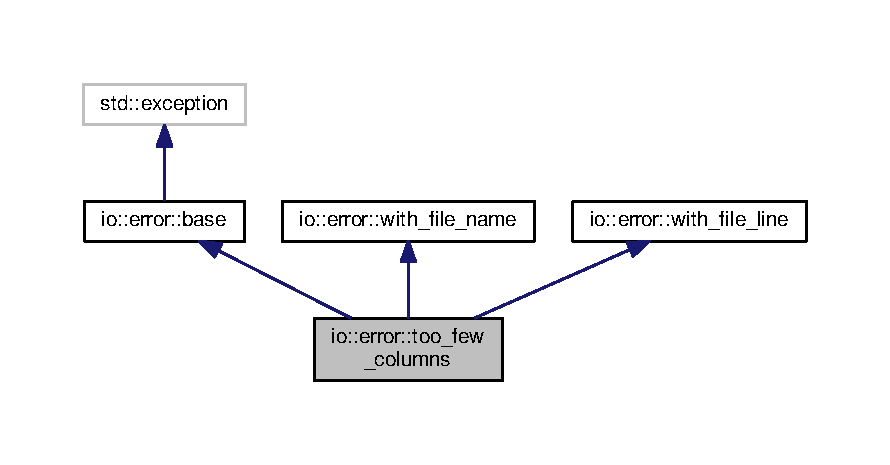
\includegraphics[width=350pt]{structio_1_1error_1_1too__few__columns__inherit__graph}
\end{center}
\end{figure}


Collaboration diagram for io\+:\+:error\+:\+:too\+\_\+few\+\_\+columns\+:\nopagebreak
\begin{figure}[H]
\begin{center}
\leavevmode
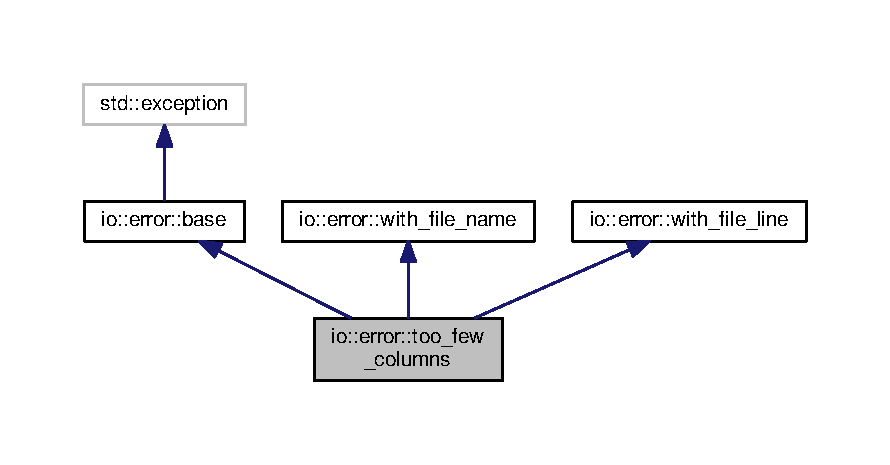
\includegraphics[width=350pt]{structio_1_1error_1_1too__few__columns__coll__graph}
\end{center}
\end{figure}
\subsection*{Public Member Functions}
\begin{DoxyCompactItemize}
\item 
void {\bfseries format\+\_\+error\+\_\+message} () const \label{structio_1_1error_1_1too__few__columns_a208e2be6855a6bfd1f3792be146dd84f}

\end{DoxyCompactItemize}
\subsection*{Additional Inherited Members}


The documentation for this struct was generated from the following file\+:\begin{DoxyCompactItemize}
\item 
csv.\+h\end{DoxyCompactItemize}

\section{io\+:\+:error\+:\+:too\+\_\+many\+\_\+columns Struct Reference}
\label{structio_1_1error_1_1too__many__columns}\index{io\+::error\+::too\+\_\+many\+\_\+columns@{io\+::error\+::too\+\_\+many\+\_\+columns}}


Inheritance diagram for io\+:\+:error\+:\+:too\+\_\+many\+\_\+columns\+:\nopagebreak
\begin{figure}[H]
\begin{center}
\leavevmode
\includegraphics[width=350pt]{structio_1_1error_1_1too__many__columns__inherit__graph}
\end{center}
\end{figure}


Collaboration diagram for io\+:\+:error\+:\+:too\+\_\+many\+\_\+columns\+:\nopagebreak
\begin{figure}[H]
\begin{center}
\leavevmode
\includegraphics[width=350pt]{structio_1_1error_1_1too__many__columns__coll__graph}
\end{center}
\end{figure}
\subsection*{Public Member Functions}
\begin{DoxyCompactItemize}
\item 
void {\bfseries format\+\_\+error\+\_\+message} () const \label{structio_1_1error_1_1too__many__columns_ad5cc8b4251752fec054163a9d6d0876a}

\end{DoxyCompactItemize}
\subsection*{Additional Inherited Members}


The documentation for this struct was generated from the following file\+:\begin{DoxyCompactItemize}
\item 
csv.\+h\end{DoxyCompactItemize}

\section{io\+:\+:trim\+\_\+chars$<$ trim\+\_\+char\+\_\+list $>$ Struct Template Reference}
\label{structio_1_1trim__chars}\index{io\+::trim\+\_\+chars$<$ trim\+\_\+char\+\_\+list $>$@{io\+::trim\+\_\+chars$<$ trim\+\_\+char\+\_\+list $>$}}
\subsection*{Static Public Member Functions}
\begin{DoxyCompactItemize}
\item 
static void {\bfseries trim} (char $\ast$\&str\+\_\+begin, char $\ast$\&str\+\_\+end)\label{structio_1_1trim__chars_a4cffc5e839ab4024ca8c8330e26e338c}

\end{DoxyCompactItemize}


The documentation for this struct was generated from the following file\+:\begin{DoxyCompactItemize}
\item 
csv.\+h\end{DoxyCompactItemize}

\section{user\+Interface Class Reference}
\label{classuser_interface}\index{user\+Interface@{user\+Interface}}
\subsection*{Public Member Functions}
\begin{DoxyCompactItemize}
\item 
{\bf user\+Interface} ()
\item 
void {\bfseries menu} ()\label{classuser_interface_a749647fc96b7d6183f172b2477019b6f}

\item 
void {\bfseries file\+Handler} ()\label{classuser_interface_a30de9d3694761c1057ad89eb4b7ecd99}

\item 
void {\bfseries maintenence} ()\label{classuser_interface_a2f0cfe4b8dafe9d2c3d18cd618a58408}

\item 
void {\bfseries add\+User\+Files} ()\label{classuser_interface_a14b008db1bc3e8dabaaac30b7abd0059}

\item 
void {\bfseries clear\+Data} ()\label{classuser_interface_a7e5279e745e02ace19344bde1bb141ed}

\item 
void {\bfseries search} ()\label{classuser_interface_afe1449a33f038a35d08cec62b7927434}

\end{DoxyCompactItemize}


\subsection{Constructor \& Destructor Documentation}
\index{user\+Interface@{user\+Interface}!user\+Interface@{user\+Interface}}
\index{user\+Interface@{user\+Interface}!user\+Interface@{user\+Interface}}
\subsubsection[{user\+Interface()}]{\setlength{\rightskip}{0pt plus 5cm}user\+Interface\+::user\+Interface (
\begin{DoxyParamCaption}
{}
\end{DoxyParamCaption}
)\hspace{0.3cm}{\ttfamily [inline]}}\label{classuser_interface_a309613e7ac0dcdbbc74c722132bcef3d}
Document\+Parser W\+I\+TH read\+In\+All\+Files(); get\+Top50\+Words(); read\+In\+Tag\+File(string); read\+In\+Ques\+File(string); Once Query is implemented (after we can read in all data),
\begin{DoxyItemize}
\item search(string);
\item open\+At\+Search(int);
\item print\+All\+Queries(); $^\wedge$$^\wedge$$^\wedge$\+This all will be my responsibility (T\+HE Q\+U\+E\+RY). Just have a function that calls that function in the Query\+Processor
\end{DoxyItemize}

The documentation for this class was generated from the following file\+:\begin{DoxyCompactItemize}
\item 
userinterface\+\_\+non\+G\+U\+I.\+h\end{DoxyCompactItemize}

\section{io\+:\+:error\+:\+:with\+\_\+column\+\_\+content Struct Reference}
\label{structio_1_1error_1_1with__column__content}\index{io\+::error\+::with\+\_\+column\+\_\+content@{io\+::error\+::with\+\_\+column\+\_\+content}}


Inheritance diagram for io\+:\+:error\+:\+:with\+\_\+column\+\_\+content\+:\nopagebreak
\begin{figure}[H]
\begin{center}
\leavevmode
\includegraphics[width=324pt]{structio_1_1error_1_1with__column__content__inherit__graph}
\end{center}
\end{figure}
\subsection*{Public Member Functions}
\begin{DoxyCompactItemize}
\item 
void {\bfseries set\+\_\+column\+\_\+content} (const char $\ast$column\+\_\+content)\label{structio_1_1error_1_1with__column__content_ae7375310dc02425cb3cc4115b3ac8d6a}

\end{DoxyCompactItemize}
\subsection*{Public Attributes}
\begin{DoxyCompactItemize}
\item 
char {\bfseries column\+\_\+content} [max\+\_\+column\+\_\+content\+\_\+length+1]\label{structio_1_1error_1_1with__column__content_a8587779769fbfb40155abb362137a523}

\end{DoxyCompactItemize}


The documentation for this struct was generated from the following file\+:\begin{DoxyCompactItemize}
\item 
csv.\+h\end{DoxyCompactItemize}

\section{io\+:\+:error\+:\+:with\+\_\+column\+\_\+name Struct Reference}
\label{structio_1_1error_1_1with__column__name}\index{io\+::error\+::with\+\_\+column\+\_\+name@{io\+::error\+::with\+\_\+column\+\_\+name}}


Inheritance diagram for io\+:\+:error\+:\+:with\+\_\+column\+\_\+name\+:\nopagebreak
\begin{figure}[H]
\begin{center}
\leavevmode
\includegraphics[width=350pt]{structio_1_1error_1_1with__column__name__inherit__graph}
\end{center}
\end{figure}
\subsection*{Public Member Functions}
\begin{DoxyCompactItemize}
\item 
void {\bfseries set\+\_\+column\+\_\+name} (const char $\ast$column\+\_\+name)\label{structio_1_1error_1_1with__column__name_a2a8144d3591a4bb618368ca7261befef}

\end{DoxyCompactItemize}
\subsection*{Public Attributes}
\begin{DoxyCompactItemize}
\item 
char {\bfseries column\+\_\+name} [max\+\_\+column\+\_\+name\+\_\+length+1]\label{structio_1_1error_1_1with__column__name_af40ba00f1f035d363b099baf1f724323}

\end{DoxyCompactItemize}


The documentation for this struct was generated from the following file\+:\begin{DoxyCompactItemize}
\item 
csv.\+h\end{DoxyCompactItemize}

\section{io\+:\+:error\+:\+:with\+\_\+errno Struct Reference}
\label{structio_1_1error_1_1with__errno}\index{io\+::error\+::with\+\_\+errno@{io\+::error\+::with\+\_\+errno}}


Inheritance diagram for io\+:\+:error\+:\+:with\+\_\+errno\+:\nopagebreak
\begin{figure}[H]
\begin{center}
\leavevmode
\includegraphics[width=181pt]{structio_1_1error_1_1with__errno__inherit__graph}
\end{center}
\end{figure}
\subsection*{Public Member Functions}
\begin{DoxyCompactItemize}
\item 
void {\bfseries set\+\_\+errno} (int errno\+\_\+value)\label{structio_1_1error_1_1with__errno_a572cfa4b4a96792cd1d17dc9ad2eb5a9}

\end{DoxyCompactItemize}
\subsection*{Public Attributes}
\begin{DoxyCompactItemize}
\item 
int {\bfseries errno\+\_\+value}\label{structio_1_1error_1_1with__errno_a99dcacba02cb53351fe64d7e064406be}

\end{DoxyCompactItemize}


The documentation for this struct was generated from the following file\+:\begin{DoxyCompactItemize}
\item 
csv.\+h\end{DoxyCompactItemize}

\section{io\+:\+:error\+:\+:with\+\_\+file\+\_\+line Struct Reference}
\label{structio_1_1error_1_1with__file__line}\index{io\+::error\+::with\+\_\+file\+\_\+line@{io\+::error\+::with\+\_\+file\+\_\+line}}


Inheritance diagram for io\+:\+:error\+:\+:with\+\_\+file\+\_\+line\+:\nopagebreak
\begin{figure}[H]
\begin{center}
\leavevmode
\includegraphics[width=330pt]{structio_1_1error_1_1with__file__line__inherit__graph}
\end{center}
\end{figure}
\subsection*{Public Member Functions}
\begin{DoxyCompactItemize}
\item 
void {\bfseries set\+\_\+file\+\_\+line} (int file\+\_\+line)\label{structio_1_1error_1_1with__file__line_aa92778a81778abc676ec6ee9952bba8c}

\end{DoxyCompactItemize}
\subsection*{Public Attributes}
\begin{DoxyCompactItemize}
\item 
int {\bfseries file\+\_\+line}\label{structio_1_1error_1_1with__file__line_a391298c37172bcdb83aeb3daf65d5a0e}

\end{DoxyCompactItemize}


The documentation for this struct was generated from the following file\+:\begin{DoxyCompactItemize}
\item 
csv.\+h\end{DoxyCompactItemize}

\section{io\+:\+:error\+:\+:with\+\_\+file\+\_\+name Struct Reference}
\label{structio_1_1error_1_1with__file__name}\index{io\+::error\+::with\+\_\+file\+\_\+name@{io\+::error\+::with\+\_\+file\+\_\+name}}


Inheritance diagram for io\+:\+:error\+:\+:with\+\_\+file\+\_\+name\+:\nopagebreak
\begin{figure}[H]
\begin{center}
\leavevmode
\includegraphics[height=550pt]{structio_1_1error_1_1with__file__name__inherit__graph}
\end{center}
\end{figure}
\subsection*{Public Member Functions}
\begin{DoxyCompactItemize}
\item 
void {\bfseries set\+\_\+file\+\_\+name} (const char $\ast$file\+\_\+name)\label{structio_1_1error_1_1with__file__name_ae765de62778c989d4658b4efe2995390}

\end{DoxyCompactItemize}
\subsection*{Public Attributes}
\begin{DoxyCompactItemize}
\item 
char {\bfseries file\+\_\+name} [max\+\_\+file\+\_\+name\+\_\+length+1]\label{structio_1_1error_1_1with__file__name_ac957d5590a8b95517b74eb5bf373a424}

\end{DoxyCompactItemize}


The documentation for this struct was generated from the following file\+:\begin{DoxyCompactItemize}
\item 
csv.\+h\end{DoxyCompactItemize}

\section{word Class Reference}
\label{classword}\index{word@{word}}


Collaboration diagram for word\+:\nopagebreak
\begin{figure}[H]
\begin{center}
\leavevmode
\includegraphics[width=212pt]{classword__coll__graph}
\end{center}
\end{figure}
\subsection*{Public Member Functions}
\begin{DoxyCompactItemize}
\item 
{\bf word} ()\label{classword_a2a7bb6f6fcfd45d7f5137b53a97e23b8}

\begin{DoxyCompactList}\small\item\em word \end{DoxyCompactList}\item 
{\bf word} (string \&input, int input\+ID, int freq)
\begin{DoxyCompactList}\small\item\em word \end{DoxyCompactList}\item 
void {\bf update\+Freq} (int \&input\+ID)
\begin{DoxyCompactList}\small\item\em update\+Freq \end{DoxyCompactList}\item 
void {\bf update\+Tag\+Freq} (int \&input\+ID)
\begin{DoxyCompactList}\small\item\em update\+Tag\+Freq \end{DoxyCompactList}\item 
void {\bf print} ()\label{classword_a3a5f547cab6e1814ef96b39003a0c472}

\begin{DoxyCompactList}\small\item\em print Prints all word values that are sorted by freuency \end{DoxyCompactList}\item 
void {\bf swap} (int $\ast$a, int $\ast$b)
\begin{DoxyCompactList}\small\item\em swap \end{DoxyCompactList}\item 
void {\bf q\+Sort} (int left, int right)
\begin{DoxyCompactList}\small\item\em q\+Sort \end{DoxyCompactList}\item 
void {\bf q\+Sort} ()\label{classword_a4f51a299447e14954a66f2ae1492c0a7}

\begin{DoxyCompactList}\small\item\em q\+Sort \end{DoxyCompactList}\end{DoxyCompactItemize}
\subsection*{Public Attributes}
\begin{DoxyCompactItemize}
\item 
vector$<$ int $>$ {\bfseries id\+List}\label{classword_a1547d07b9aab776435e23bc7e9e0581e}

\item 
vector$<$ int $>$ {\bfseries freq\+List}\label{classword_aef3844fe2f6bfb468a65322d6d6ef9e6}

\item 
string {\bfseries word\+Value} = \char`\"{} \char`\"{}\label{classword_a23fcaa1a4e81f137e0b5c46cead8a311}

\end{DoxyCompactItemize}


\subsection{Constructor \& Destructor Documentation}
\index{word@{word}!word@{word}}
\index{word@{word}!word@{word}}
\subsubsection[{word(string \&input, int input\+I\+D, int freq)}]{\setlength{\rightskip}{0pt plus 5cm}word\+::word (
\begin{DoxyParamCaption}
\item[{string \&}]{input, }
\item[{int}]{input\+ID, }
\item[{int}]{freq}
\end{DoxyParamCaption}
)\hspace{0.3cm}{\ttfamily [inline]}}\label{classword_a898c3e08927dc1eb947ab311f0ad153b}


word 


\begin{DoxyParams}{Parameters}
{\em input} & \\
\hline
{\em input\+ID} & \\
\hline
{\em freq} & \\
\hline
\end{DoxyParams}


\subsection{Member Function Documentation}
\index{word@{word}!q\+Sort@{q\+Sort}}
\index{q\+Sort@{q\+Sort}!word@{word}}
\subsubsection[{q\+Sort(int left, int right)}]{\setlength{\rightskip}{0pt plus 5cm}void word\+::q\+Sort (
\begin{DoxyParamCaption}
\item[{int}]{left, }
\item[{int}]{right}
\end{DoxyParamCaption}
)\hspace{0.3cm}{\ttfamily [inline]}}\label{classword_abbc538aef21fabaa9d893810c0fd6057}


q\+Sort 


\begin{DoxyParams}{Parameters}
{\em left} & \\
\hline
{\em right} & Sorting functions for relevancy rankings Uses Sprint 3 algorithm for sorting vectors (In D\+S\+Vector) \\
\hline
\end{DoxyParams}
\index{word@{word}!swap@{swap}}
\index{swap@{swap}!word@{word}}
\subsubsection[{swap(int $\ast$a, int $\ast$b)}]{\setlength{\rightskip}{0pt plus 5cm}void word\+::swap (
\begin{DoxyParamCaption}
\item[{int $\ast$}]{a, }
\item[{int $\ast$}]{b}
\end{DoxyParamCaption}
)\hspace{0.3cm}{\ttfamily [inline]}}\label{classword_ad8f1a62dce2c180926bc9973e9b0f0dd}


swap 


\begin{DoxyParams}{Parameters}
{\em a} & \\
\hline
{\em b} & \\
\hline
\end{DoxyParams}
\index{word@{word}!update\+Freq@{update\+Freq}}
\index{update\+Freq@{update\+Freq}!word@{word}}
\subsubsection[{update\+Freq(int \&input\+I\+D)}]{\setlength{\rightskip}{0pt plus 5cm}void word\+::update\+Freq (
\begin{DoxyParamCaption}
\item[{int \&}]{input\+ID}
\end{DoxyParamCaption}
)\hspace{0.3cm}{\ttfamily [inline]}}\label{classword_a61cf10a20f6e69cbfe753089f11a9c2b}


update\+Freq 


\begin{DoxyParams}{Parameters}
{\em input\+ID} & Updates word frequency with +1(for word) if it is contained in the hash table \\
\hline
\end{DoxyParams}
\index{word@{word}!update\+Tag\+Freq@{update\+Tag\+Freq}}
\index{update\+Tag\+Freq@{update\+Tag\+Freq}!word@{word}}
\subsubsection[{update\+Tag\+Freq(int \&input\+I\+D)}]{\setlength{\rightskip}{0pt plus 5cm}void word\+::update\+Tag\+Freq (
\begin{DoxyParamCaption}
\item[{int \&}]{input\+ID}
\end{DoxyParamCaption}
)\hspace{0.3cm}{\ttfamily [inline]}}\label{classword_aefdd440b53f841b292bffeb4189c0ef6}


update\+Tag\+Freq 


\begin{DoxyParams}{Parameters}
{\em input\+ID} & Updates word frequency with +5(for tag) if it is contained in the hash table \\
\hline
\end{DoxyParams}


The documentation for this class was generated from the following file\+:\begin{DoxyCompactItemize}
\item 
word.\+h\end{DoxyCompactItemize}

\chapter{File Documentation}
\section{porter2\+\_\+stemmer.\+cpp File Reference}
\label{porter2__stemmer_8cpp}\index{porter2\+\_\+stemmer.\+cpp@{porter2\+\_\+stemmer.\+cpp}}
{\ttfamily \#include $<$algorithm$>$}\\*
{\ttfamily \#include $<$utility$>$}\\*
{\ttfamily \#include $<$iostream$>$}\\*
{\ttfamily \#include $<$sstream$>$}\\*
{\ttfamily \#include $<$unordered\+\_\+map$>$}\\*
{\ttfamily \#include \char`\"{}porter2\+\_\+stemmer.\+h\char`\"{}}\\*
Include dependency graph for porter2\+\_\+stemmer.\+cpp\+:\nopagebreak
\begin{figure}[H]
\begin{center}
\leavevmode
\includegraphics[width=350pt]{porter2__stemmer_8cpp__incl}
\end{center}
\end{figure}


\subsection{Detailed Description}
\begin{DoxyAuthor}{Author}
Sean Massung 
\end{DoxyAuthor}
\begin{DoxyDate}{Date}
September 2012
\end{DoxyDate}
Implementation of {\tt http\+://snowball.\+tartarus.\+org/algorithms/english/stemmer.\+html}

Copyright (C) 2012 Sean Massung

Permission is hereby granted, free of charge, to any person obtaining a copy of this software and associated documentation files (the \char`\"{}\+Software\char`\"{}), to deal in the Software without restriction, including without limitation the rights to use, copy, modify, merge, publish, distribute, sublicense, and/or sell copies of the Software, and to permit persons to whom the Software is furnished to do so, subject to the following conditions\+:

The above copyright notice and this permission notice shall be included in all copies or substantial portions of the Software.

T\+HE S\+O\+F\+T\+W\+A\+RE IS P\+R\+O\+V\+I\+D\+ED \char`\"{}\+A\+S I\+S\char`\"{}, W\+I\+T\+H\+O\+UT W\+A\+R\+R\+A\+N\+TY OF A\+NY K\+I\+ND, E\+X\+P\+R\+E\+SS OR I\+M\+P\+L\+I\+ED, I\+N\+C\+L\+U\+D\+I\+NG B\+UT N\+OT L\+I\+M\+I\+T\+ED TO T\+HE W\+A\+R\+R\+A\+N\+T\+I\+ES OF M\+E\+R\+C\+H\+A\+N\+T\+A\+B\+I\+L\+I\+TY, F\+I\+T\+N\+E\+SS F\+OR A P\+A\+R\+T\+I\+C\+U\+L\+AR P\+U\+R\+P\+O\+SE A\+ND N\+O\+N\+I\+N\+F\+R\+I\+N\+G\+E\+M\+E\+NT. IN NO E\+V\+E\+NT S\+H\+A\+LL T\+HE A\+U\+T\+H\+O\+RS OR C\+O\+P\+Y\+R\+I\+G\+HT H\+O\+L\+D\+E\+RS BE L\+I\+A\+B\+LE F\+OR A\+NY C\+L\+A\+IM, D\+A\+M\+A\+G\+ES OR O\+T\+H\+ER L\+I\+A\+B\+I\+L\+I\+TY, W\+H\+E\+T\+H\+ER IN AN A\+C\+T\+I\+ON OF C\+O\+N\+T\+R\+A\+CT, T\+O\+RT OR O\+T\+H\+E\+R\+W\+I\+SE, A\+R\+I\+S\+I\+NG F\+R\+OM, O\+UT OF OR IN C\+O\+N\+N\+E\+C\+T\+I\+ON W\+I\+TH T\+HE S\+O\+F\+T\+W\+A\+RE OR T\+HE U\+SE OR O\+T\+H\+ER D\+E\+A\+L\+I\+N\+GS IN T\+HE S\+O\+F\+T\+W\+A\+RE. 
\section{porter2\+\_\+stemmer.\+h File Reference}
\label{porter2__stemmer_8h}\index{porter2\+\_\+stemmer.\+h@{porter2\+\_\+stemmer.\+h}}
{\ttfamily \#include $<$vector$>$}\\*
{\ttfamily \#include $<$string$>$}\\*
Include dependency graph for porter2\+\_\+stemmer.\+h\+:\nopagebreak
\begin{figure}[H]
\begin{center}
\leavevmode
\includegraphics[width=184pt]{porter2__stemmer_8h__incl}
\end{center}
\end{figure}
This graph shows which files directly or indirectly include this file\+:\nopagebreak
\begin{figure}[H]
\begin{center}
\leavevmode
\includegraphics[width=189pt]{porter2__stemmer_8h__dep__incl}
\end{center}
\end{figure}
\subsection*{Functions}
\begin{DoxyCompactItemize}
\item 
void {\bfseries Porter2\+Stemmer\+::stem} (std\+::string \&{\bf word})\label{porter2__stemmer_8h_ad07c4652a1144329db4bdfb6ce640d80}

\item 
void {\bfseries Porter2\+Stemmer\+::trim} (std\+::string \&{\bf word})\label{porter2__stemmer_8h_ac74222c2eb041cff861fddfd529bc983}

\item 
size\+\_\+t {\bfseries Porter2\+Stemmer\+::internal\+::first\+Non\+Vowel\+After\+Vowel} (const std\+::string \&{\bf word}, size\+\_\+t start)\label{porter2__stemmer_8h_a4419080bc3b64aca4998a732e9f99d84}

\item 
size\+\_\+t {\bfseries Porter2\+Stemmer\+::internal\+::get\+Start\+R1} (const std\+::string \&{\bf word})\label{porter2__stemmer_8h_a2d7e133e04950f30c9b3a2935be7c802}

\item 
size\+\_\+t {\bfseries Porter2\+Stemmer\+::internal\+::get\+Start\+R2} (const std\+::string \&{\bf word}, size\+\_\+t start\+R1)\label{porter2__stemmer_8h_a87bb0a5733b6267185b7951349477070}

\item 
void {\bfseries Porter2\+Stemmer\+::internal\+::changeY} (std\+::string \&{\bf word})\label{porter2__stemmer_8h_add0f2aec57b66845cb78e98844bb4205}

\item 
void {\bf Porter2\+Stemmer\+::internal\+::step0} (std\+::string \&{\bf word})
\item 
bool {\bf Porter2\+Stemmer\+::internal\+::step1A} (std\+::string \&{\bf word})
\item 
void {\bf Porter2\+Stemmer\+::internal\+::step1B} (std\+::string \&{\bf word}, size\+\_\+t start\+R1)
\item 
void {\bf Porter2\+Stemmer\+::internal\+::step1C} (std\+::string \&{\bf word})
\item 
void {\bf Porter2\+Stemmer\+::internal\+::step2} (std\+::string \&{\bf word}, size\+\_\+t start\+R1)
\item 
void {\bf Porter2\+Stemmer\+::internal\+::step3} (std\+::string \&{\bf word}, size\+\_\+t start\+R1, size\+\_\+t start\+R2)
\item 
void {\bf Porter2\+Stemmer\+::internal\+::step4} (std\+::string \&{\bf word}, size\+\_\+t start\+R2)
\item 
void {\bf Porter2\+Stemmer\+::internal\+::step5} (std\+::string \&{\bf word}, size\+\_\+t start\+R1, size\+\_\+t start\+R2)
\item 
bool {\bf Porter2\+Stemmer\+::internal\+::is\+Short} (const std\+::string \&{\bf word})
\item 
bool {\bfseries Porter2\+Stemmer\+::internal\+::special} (std\+::string \&{\bf word})\label{porter2__stemmer_8h_a7c20680dfe258c8050c8225d97b2e160}

\item 
bool {\bfseries Porter2\+Stemmer\+::internal\+::is\+Vowel} (char ch)\label{porter2__stemmer_8h_a63d428e12b7b2aeea945c24afe44d1d2}

\item 
bool {\bfseries Porter2\+Stemmer\+::internal\+::is\+VowelY} (char ch)\label{porter2__stemmer_8h_a72ec1ef1732191be64f203bbe0e4397d}

\item 
bool {\bfseries Porter2\+Stemmer\+::internal\+::ends\+With} (const std\+::string \&{\bf word}, const std\+::string \&str)\label{porter2__stemmer_8h_a08785aaf007de16789d1cbc50a6d72b4}

\item 
bool {\bfseries Porter2\+Stemmer\+::internal\+::ends\+In\+Double} (const std\+::string \&{\bf word})\label{porter2__stemmer_8h_aca68167dfec7979b35d5bc732d2c6ef0}

\item 
bool {\bfseries Porter2\+Stemmer\+::internal\+::replace\+If\+Exists} (std\+::string \&{\bf word}, const std\+::string \&suffix, const std\+::string \&replacement, size\+\_\+t start)\label{porter2__stemmer_8h_aff7926ca225a004069d681b88826a73a}

\item 
bool {\bfseries Porter2\+Stemmer\+::internal\+::is\+Valid\+L\+I\+Ending} (char ch)\label{porter2__stemmer_8h_acb88f8cc716be69a9c19818473614d68}

\item 
bool {\bfseries Porter2\+Stemmer\+::internal\+::contains\+Vowel} (const std\+::string \&{\bf word}, size\+\_\+t start, size\+\_\+t end)\label{porter2__stemmer_8h_ade420031f6e4e4a9f432c82b7f54420b}

\end{DoxyCompactItemize}


\subsection{Detailed Description}
\begin{DoxyAuthor}{Author}
Sean Massung 
\end{DoxyAuthor}
\begin{DoxyDate}{Date}
September 2012
\end{DoxyDate}
Implementation of {\tt http\+://snowball.\+tartarus.\+org/algorithms/english/stemmer.\+html}

Copyright (C) 2012 Sean Massung

Permission is hereby granted, free of charge, to any person obtaining a copy of this software and associated documentation files (the \char`\"{}\+Software\char`\"{}), to deal in the Software without restriction, including without limitation the rights to use, copy, modify, merge, publish, distribute, sublicense, and/or sell copies of the Software, and to permit persons to whom the Software is furnished to do so, subject to the following conditions\+:

The above copyright notice and this permission notice shall be included in all copies or substantial portions of the Software.

T\+HE S\+O\+F\+T\+W\+A\+RE IS P\+R\+O\+V\+I\+D\+ED \char`\"{}\+A\+S I\+S\char`\"{}, W\+I\+T\+H\+O\+UT W\+A\+R\+R\+A\+N\+TY OF A\+NY K\+I\+ND, E\+X\+P\+R\+E\+SS OR I\+M\+P\+L\+I\+ED, I\+N\+C\+L\+U\+D\+I\+NG B\+UT N\+OT L\+I\+M\+I\+T\+ED TO T\+HE W\+A\+R\+R\+A\+N\+T\+I\+ES OF M\+E\+R\+C\+H\+A\+N\+T\+A\+B\+I\+L\+I\+TY, F\+I\+T\+N\+E\+SS F\+OR A P\+A\+R\+T\+I\+C\+U\+L\+AR P\+U\+R\+P\+O\+SE A\+ND N\+O\+N\+I\+N\+F\+R\+I\+N\+G\+E\+M\+E\+NT. IN NO E\+V\+E\+NT S\+H\+A\+LL T\+HE A\+U\+T\+H\+O\+RS OR C\+O\+P\+Y\+R\+I\+G\+HT H\+O\+L\+D\+E\+RS BE L\+I\+A\+B\+LE F\+OR A\+NY C\+L\+A\+IM, D\+A\+M\+A\+G\+ES OR O\+T\+H\+ER L\+I\+A\+B\+I\+L\+I\+TY, W\+H\+E\+T\+H\+ER IN AN A\+C\+T\+I\+ON OF C\+O\+N\+T\+R\+A\+CT, T\+O\+RT OR O\+T\+H\+E\+R\+W\+I\+SE, A\+R\+I\+S\+I\+NG F\+R\+OM, O\+UT OF OR IN C\+O\+N\+N\+E\+C\+T\+I\+ON W\+I\+TH T\+HE S\+O\+F\+T\+W\+A\+RE OR T\+HE U\+SE OR O\+T\+H\+ER D\+E\+A\+L\+I\+N\+GS IN T\+HE S\+O\+F\+T\+W\+A\+RE. 

\subsection{Function Documentation}
\index{porter2\+\_\+stemmer.\+h@{porter2\+\_\+stemmer.\+h}!is\+Short@{is\+Short}}
\index{is\+Short@{is\+Short}!porter2\+\_\+stemmer.\+h@{porter2\+\_\+stemmer.\+h}}
\subsubsection[{is\+Short(const std\+::string \&word)}]{\setlength{\rightskip}{0pt plus 5cm}bool Porter2\+Stemmer\+::internal\+::is\+Short (
\begin{DoxyParamCaption}
\item[{const std\+::string \&}]{word}
\end{DoxyParamCaption}
)\hspace{0.3cm}{\ttfamily [inline]}}\label{porter2__stemmer_8h_file_a15dc6085d05bf8e2ee691ef08e0fae29}
Determines whether a word ends in a short syllable. Define a short syllable in a word as either

(a) a vowel followed by a non-\/vowel other than w, x or Y and preceded by a non-\/vowel (b) a vowel at the beginning of the word followed by a non-\/vowel. 

Here is the call graph for this function\+:\nopagebreak
\begin{figure}[H]
\begin{center}
\leavevmode
\includegraphics[width=205pt]{porter2__stemmer_8h_a15dc6085d05bf8e2ee691ef08e0fae29_cgraph}
\end{center}
\end{figure}




Here is the caller graph for this function\+:\nopagebreak
\begin{figure}[H]
\begin{center}
\leavevmode
\includegraphics[width=350pt]{porter2__stemmer_8h_a15dc6085d05bf8e2ee691ef08e0fae29_icgraph}
\end{center}
\end{figure}


\index{porter2\+\_\+stemmer.\+h@{porter2\+\_\+stemmer.\+h}!step0@{step0}}
\index{step0@{step0}!porter2\+\_\+stemmer.\+h@{porter2\+\_\+stemmer.\+h}}
\subsubsection[{step0(std\+::string \&word)}]{\setlength{\rightskip}{0pt plus 5cm}void Porter2\+Stemmer\+::internal\+::step0 (
\begin{DoxyParamCaption}
\item[{std\+::string \&}]{word}
\end{DoxyParamCaption}
)}\label{porter2__stemmer_8h_file_ae689551ae90968445d4ab1a60ffc805c}
Step 0 

Here is the call graph for this function\+:\nopagebreak
\begin{figure}[H]
\begin{center}
\leavevmode
\includegraphics[width=205pt]{porter2__stemmer_8h_ae689551ae90968445d4ab1a60ffc805c_cgraph}
\end{center}
\end{figure}




Here is the caller graph for this function\+:\nopagebreak
\begin{figure}[H]
\begin{center}
\leavevmode
\includegraphics[width=205pt]{porter2__stemmer_8h_ae689551ae90968445d4ab1a60ffc805c_icgraph}
\end{center}
\end{figure}


\index{porter2\+\_\+stemmer.\+h@{porter2\+\_\+stemmer.\+h}!step1A@{step1A}}
\index{step1A@{step1A}!porter2\+\_\+stemmer.\+h@{porter2\+\_\+stemmer.\+h}}
\subsubsection[{step1\+A(std\+::string \&word)}]{\setlength{\rightskip}{0pt plus 5cm}bool Porter2\+Stemmer\+::internal\+::step1A (
\begin{DoxyParamCaption}
\item[{std\+::string \&}]{word}
\end{DoxyParamCaption}
)}\label{porter2__stemmer_8h_file_af0acc908e606cd6e2917bf2ed31d5fe7}
Step 1a\+:

sses replace by ss

ied ies replace by i if preceded by more than one letter, otherwise by ie (so ties -\/$>$ tie, cries -\/$>$ cri)

us ss do nothing

s delete if the preceding word part contains a vowel not immediately before the s (so gas and this retain the s, gaps and kiwis lose it) 

Here is the call graph for this function\+:\nopagebreak
\begin{figure}[H]
\begin{center}
\leavevmode
\includegraphics[width=205pt]{porter2__stemmer_8h_af0acc908e606cd6e2917bf2ed31d5fe7_cgraph}
\end{center}
\end{figure}




Here is the caller graph for this function\+:\nopagebreak
\begin{figure}[H]
\begin{center}
\leavevmode
\includegraphics[width=205pt]{porter2__stemmer_8h_af0acc908e606cd6e2917bf2ed31d5fe7_icgraph}
\end{center}
\end{figure}


\index{porter2\+\_\+stemmer.\+h@{porter2\+\_\+stemmer.\+h}!step1B@{step1B}}
\index{step1B@{step1B}!porter2\+\_\+stemmer.\+h@{porter2\+\_\+stemmer.\+h}}
\subsubsection[{step1\+B(std\+::string \&word, size\+\_\+t start\+R1)}]{\setlength{\rightskip}{0pt plus 5cm}void Porter2\+Stemmer\+::internal\+::step1B (
\begin{DoxyParamCaption}
\item[{std\+::string \&}]{word, }
\item[{size\+\_\+t}]{start\+R1}
\end{DoxyParamCaption}
)}\label{porter2__stemmer_8h_file_af4cffda4b443475c766407d60eac03dc}
Step 1b\+:

eed eedly replace by ee if in R1

ed edly ing ingly delete if the preceding word part contains a vowel, and after the deletion\+: if the word ends at, bl or iz add e (so luxuriat -\/$>$ luxuriate), or if the word ends with a double remove the last letter (so hopp -\/$>$ hop), or if the word is short, add e (so hop -\/$>$ hope) 

Here is the call graph for this function\+:\nopagebreak
\begin{figure}[H]
\begin{center}
\leavevmode
\includegraphics[width=350pt]{porter2__stemmer_8h_af4cffda4b443475c766407d60eac03dc_cgraph}
\end{center}
\end{figure}




Here is the caller graph for this function\+:\nopagebreak
\begin{figure}[H]
\begin{center}
\leavevmode
\includegraphics[width=205pt]{porter2__stemmer_8h_af4cffda4b443475c766407d60eac03dc_icgraph}
\end{center}
\end{figure}


\index{porter2\+\_\+stemmer.\+h@{porter2\+\_\+stemmer.\+h}!step1C@{step1C}}
\index{step1C@{step1C}!porter2\+\_\+stemmer.\+h@{porter2\+\_\+stemmer.\+h}}
\subsubsection[{step1\+C(std\+::string \&word)}]{\setlength{\rightskip}{0pt plus 5cm}void Porter2\+Stemmer\+::internal\+::step1C (
\begin{DoxyParamCaption}
\item[{std\+::string \&}]{word}
\end{DoxyParamCaption}
)}\label{porter2__stemmer_8h_file_abc52eb93a0acc99087ca62bb2a4e647e}
Step 1c\+:

Replace suffix y or Y by i if preceded by a non-\/vowel which is not the first letter of the word (so cry -\/$>$ cri, by -\/$>$ by, say -\/$>$ say) 

Here is the call graph for this function\+:\nopagebreak
\begin{figure}[H]
\begin{center}
\leavevmode
\includegraphics[width=205pt]{porter2__stemmer_8h_abc52eb93a0acc99087ca62bb2a4e647e_cgraph}
\end{center}
\end{figure}




Here is the caller graph for this function\+:\nopagebreak
\begin{figure}[H]
\begin{center}
\leavevmode
\includegraphics[width=205pt]{porter2__stemmer_8h_abc52eb93a0acc99087ca62bb2a4e647e_icgraph}
\end{center}
\end{figure}


\index{porter2\+\_\+stemmer.\+h@{porter2\+\_\+stemmer.\+h}!step2@{step2}}
\index{step2@{step2}!porter2\+\_\+stemmer.\+h@{porter2\+\_\+stemmer.\+h}}
\subsubsection[{step2(std\+::string \&word, size\+\_\+t start\+R1)}]{\setlength{\rightskip}{0pt plus 5cm}void Porter2\+Stemmer\+::internal\+::step2 (
\begin{DoxyParamCaption}
\item[{std\+::string \&}]{word, }
\item[{size\+\_\+t}]{start\+R1}
\end{DoxyParamCaption}
)}\label{porter2__stemmer_8h_file_a8bde57d3eeee683082f53cd7a9a0a2f8}
Step 2\+:

If found and in R1, perform the action indicated.

tional\+: replace by tion enci\+: replace by ence anci\+: replace by ance abli\+: replace by able entli\+: replace by ent izer, ization\+: replace by ize ational, ation, ator\+: replace by ate alism, aliti, alli\+: replace by al fulness\+: replace by ful ousli, ousness\+: replace by ous iveness, iviti\+: replace by ive biliti, bli\+: replace by ble fulli\+: replace by ful lessli\+: replace by less ogi\+: replace by og if preceded by l li\+: delete if preceded by a valid li-\/ending 

Here is the call graph for this function\+:\nopagebreak
\begin{figure}[H]
\begin{center}
\leavevmode
\includegraphics[width=205pt]{porter2__stemmer_8h_a8bde57d3eeee683082f53cd7a9a0a2f8_cgraph}
\end{center}
\end{figure}




Here is the caller graph for this function\+:\nopagebreak
\begin{figure}[H]
\begin{center}
\leavevmode
\includegraphics[width=205pt]{porter2__stemmer_8h_a8bde57d3eeee683082f53cd7a9a0a2f8_icgraph}
\end{center}
\end{figure}


\index{porter2\+\_\+stemmer.\+h@{porter2\+\_\+stemmer.\+h}!step3@{step3}}
\index{step3@{step3}!porter2\+\_\+stemmer.\+h@{porter2\+\_\+stemmer.\+h}}
\subsubsection[{step3(std\+::string \&word, size\+\_\+t start\+R1, size\+\_\+t start\+R2)}]{\setlength{\rightskip}{0pt plus 5cm}void Porter2\+Stemmer\+::internal\+::step3 (
\begin{DoxyParamCaption}
\item[{std\+::string \&}]{word, }
\item[{size\+\_\+t}]{start\+R1, }
\item[{size\+\_\+t}]{start\+R2}
\end{DoxyParamCaption}
)}\label{porter2__stemmer_8h_file_a8ea5872c398ea38fb5ff359879613a4e}
Step 3\+:

If found and in R1, perform the action indicated.

ational\+: replace by ate tional\+: replace by tion alize\+: replace by al icate, iciti, ical\+: replace by ic ful, ness\+: delete ative\+: delete if in R2 

Here is the call graph for this function\+:\nopagebreak
\begin{figure}[H]
\begin{center}
\leavevmode
\includegraphics[width=205pt]{porter2__stemmer_8h_a8ea5872c398ea38fb5ff359879613a4e_cgraph}
\end{center}
\end{figure}




Here is the caller graph for this function\+:\nopagebreak
\begin{figure}[H]
\begin{center}
\leavevmode
\includegraphics[width=205pt]{porter2__stemmer_8h_a8ea5872c398ea38fb5ff359879613a4e_icgraph}
\end{center}
\end{figure}


\index{porter2\+\_\+stemmer.\+h@{porter2\+\_\+stemmer.\+h}!step4@{step4}}
\index{step4@{step4}!porter2\+\_\+stemmer.\+h@{porter2\+\_\+stemmer.\+h}}
\subsubsection[{step4(std\+::string \&word, size\+\_\+t start\+R2)}]{\setlength{\rightskip}{0pt plus 5cm}void Porter2\+Stemmer\+::internal\+::step4 (
\begin{DoxyParamCaption}
\item[{std\+::string \&}]{word, }
\item[{size\+\_\+t}]{start\+R2}
\end{DoxyParamCaption}
)}\label{porter2__stemmer_8h_file_a46c7932444166421508feab27b1addfa}
Step 4\+:

If found and in R2, perform the action indicated.

al ance ence er ic able ible ant ement ment ent ism ate iti ous ive ize delete ion delete if preceded by s or t 

Here is the call graph for this function\+:\nopagebreak
\begin{figure}[H]
\begin{center}
\leavevmode
\includegraphics[width=205pt]{porter2__stemmer_8h_a46c7932444166421508feab27b1addfa_cgraph}
\end{center}
\end{figure}




Here is the caller graph for this function\+:\nopagebreak
\begin{figure}[H]
\begin{center}
\leavevmode
\includegraphics[width=205pt]{porter2__stemmer_8h_a46c7932444166421508feab27b1addfa_icgraph}
\end{center}
\end{figure}


\index{porter2\+\_\+stemmer.\+h@{porter2\+\_\+stemmer.\+h}!step5@{step5}}
\index{step5@{step5}!porter2\+\_\+stemmer.\+h@{porter2\+\_\+stemmer.\+h}}
\subsubsection[{step5(std\+::string \&word, size\+\_\+t start\+R1, size\+\_\+t start\+R2)}]{\setlength{\rightskip}{0pt plus 5cm}void Porter2\+Stemmer\+::internal\+::step5 (
\begin{DoxyParamCaption}
\item[{std\+::string \&}]{word, }
\item[{size\+\_\+t}]{start\+R1, }
\item[{size\+\_\+t}]{start\+R2}
\end{DoxyParamCaption}
)}\label{porter2__stemmer_8h_file_ad53abf614a24cba562dba83857f42091}
Step 5\+:

e delete if in R2, or in R1 and not preceded by a short syllable l delete if in R2 and preceded by l 

Here is the call graph for this function\+:\nopagebreak
\begin{figure}[H]
\begin{center}
\leavevmode
\includegraphics[width=350pt]{porter2__stemmer_8h_ad53abf614a24cba562dba83857f42091_cgraph}
\end{center}
\end{figure}




Here is the caller graph for this function\+:\nopagebreak
\begin{figure}[H]
\begin{center}
\leavevmode
\includegraphics[width=205pt]{porter2__stemmer_8h_ad53abf614a24cba562dba83857f42091_icgraph}
\end{center}
\end{figure}



%--- End generated contents ---

% Index
\backmatter
\newpage
\phantomsection
\clearemptydoublepage
\addcontentsline{toc}{chapter}{Index}
\printindex

\end{document}
